\documentclass[a4paper, 12pt]{article}
\usepackage[margin=1.2in]{geometry}
\usepackage[english, ngerman]{babel}
\usepackage[autostyle]{csquotes}
\usepackage{natbib}

% \bibliographystyle{ksfh_nat}
% \bibliographystyle{apa}
\bibliographystyle{apalike}
% \bibliographystyle{plainnat}

\usepackage{hyperref}
\usepackage{graphicx}
\usepackage{titlesec}
\usepackage{subcaption}
% \usepackage[raggedrightboxes]{ragged2e}
% \usepackage{pgf-pie}
% \usepackage{pgfplots}
\usepackage[acronym, toc, numberedsection]{glossaries}
\usepackage{listings}
\usepackage{amsmath}

\lstdefinelanguage{JavaScript}{
  keywords={typeof, new, true, false, catch, function, return, null, catch, switch, var, if, in, while, do, else, case, break, const, let},
  ndkeywords={class, export, boolean, throw, implements, import, this, string, number, date},
  sensitive=false,
  comment=[l]{//},
  morecomment=[s]{/*}{*/},
  morestring=[b]',
  morestring=[b]"
}
\lstdefinestyle{mystyle}{
    % backgroundcolor=\color{backcolour},   
    commentstyle=\color{teal},
    keywordstyle=\color{red},
    ndkeywordstyle=\color{blue},
    numberstyle=\footnotesize\color{gray},
    stringstyle=\color{violet},
    % basicstyle=\ttfamily\normalsize,
    % basicstyle=\ttfamily\small,
    basicstyle=\ttfamily\footnotesize,
    breakatwhitespace=true,         
    breaklines=true,                 
    captionpos=b,                    
    % keepspaces=true,                 
    numbers=left,                    
    % numbersep=5pt,                  
    showspaces=false,                
    showstringspaces=false,
    % showtabs=false,                  
    tabsize=2,
}
\lstset{style=mystyle}

\usepackage{hyphenat}
% \hyphenation{Mathe-matik wieder-gewinnen}
\usepackage[T1]{fontenc}
\usepackage[table]{xcolor}
\usepackage[export]{adjustbox}
\usepackage{multirow}

\usepackage{newfloat}
\DeclareFloatingEnvironment[placement={!ht},name=List]{mylist}

\makenoidxglossaries
\newacronym{dom}{DOM}{Document Object Model}
\newacronym{html}{HTML}{Hypertext Markup Language}
\newacronym{css}{CSS}{Cascading Style Sheet}
\newacronym{js}{JS}{JavaScript}
\newacronym{json}{JSON}{JavaScript Object Notion}
\newacronym{csr}{CSR}{Client-side Rendering}
\newacronym{ssr}{SSR}{Server-side Rendering}
\newacronym{svg}{SVG}{Support Vector Graphic}
\newacronym{cicd}{CI/CD}{Continuous Integration and Continuous Delivery}
\newacronym{tbw}{TBW}{Total Byte Weight}
\newacronym{ttfb}{TTFB}{Time To First Byte}
\newacronym{tti}{TTI}{Time To Interactive}
\newacronym{tbt}{TBT}{Total Blocking Time}
\newacronym{lvc}{LVC}{Last Visual Change}
\newacronym{olvc}{OLVC}{Observed Last Visual Change}
\newacronym{lcp}{LCP}{Largest Contentful Paint}
\newacronym{fvc}{FVC}{First Visual Change}
\newacronym{ofvc}{OFVC}{Observed First Visual Change}
\newacronym{ovcd}{OVCD}{Observed Visual Change Duration}
\newacronym{seo}{SEO}{Search Engine Optimization}
\newacronym{pwa}{PWA}{Progressive Web App}
\newacronym{cli}{CLI}{Command Line Interface}
\newacronym{url}{URL}{Uniform Resource Locator}
\newacronym{http}{HTTP}{Hypertext Transfer Protocol}

\title{Mega-fast or just super-fast? Performance differences of mainstream JavaScript frameworks for web applications}
\author{Andreas Nicklaus}

\makeatletter

\renewenvironment{thebibliography}[1]
     {\section{References}
      \@mkboth{\MakeUppercase\bibname}{\MakeUppercase\bibname}%
      \list{\@biblabel{\@arabic\c@enumiv}}%
           {\settowidth\labelwidth{\@biblabel{#1}}%
            \leftmargin\labelwidth
            \advance\leftmargin\labelsep
            \@openbib@code
            \usecounter{enumiv}%
            \let\p@enumiv\@empty
            \renewcommand\theenumiv{\@arabic\c@enumiv}}%
      \sloppy
      \clubpenalty4000
      \@clubpenalty \clubpenalty
      \widowpenalty4000%
      \sfcode`\.\@m}
     {\def\@noitemerr
       {\@latex@warning{Empty `thebibliography' environment}}%
      \endlist}

\renewcommand\listoffigures{%
  \section{\listfigurename}%
  \@mkboth{\MakeUppercase\listfigurename}{\MakeUppercase\listfigurename}%
  \@starttoc{lof}%
}
\renewcommand\listoftables{%
  \section{\listtablename}%
  \@mkboth{\MakeUppercase\listtablename}{\MakeUppercase\listtablename}%
  \@starttoc{lot}%
}
\renewcommand\lstlistoflistings{
  \section{\lstlistlistingname}
  \@starttoc{lol}%
}
\let\Title\@title
\let\Author\@author

\rowcolors{1}{lightgray!40!}{white}

% Keywords command
\providecommand{\keywords}[1]
{
  {
    \footnotesize
    \textit{\textbf{Keywords ---} #1}
  } 
}

\makeatother

\begin{document}

\begin{titlepage}
	
  \begin{center}

    
\includegraphics[width=150px, keepaspectratio]{img/hdm-logo.png}
    
    \vspace{30px}
    {\large Masterarbeit im Studiengang Computer Science and Media}
    
    \vspace{20px}
    {\LARGE \Title}
    
    \vspace{20px}
    \noindent\rule{\textwidth}{1pt}
    
    \vspace{15px}
    vorgelegt von
    
    \vspace{10px}
    \textbf{{\large \Author}}
    
    % \vspace{5px}
    Matrikelnummer 44835
    
    \vspace{10px}
    an der Hochschule der Medien Stuttgart
    
    \vspace{10px}
    am \today
    
    \vspace{10px}
    zur Erlangung des akademischen Grades eines Master of Science
  \end{center}	
  
  \vfill
  
  {\rowcolors{1}{white}{white}\begin{tabular}[t]{ll}
    Erst-Prüfer: & Prof. Dr. Fridtjof Toenniessen \\
    Zweit-Prüfer: & Stephan Soller
  \end{tabular}}
\end{titlepage}

\selectlanguage{ngerman}

\section*{Ehrenwörtliche Erklärung}
	
	Hiermit versichere ich, \Author, ehrenwörtlich, dass ich die
	vorliegende Masterarbeit mit dem Titel: „\Title“ selbstständig und ohne fremde Hilfe verfasst und keine
	anderen als die angegebenen Hilfsmittel benutzt habe. Die Stellen der Arbeit, die dem
	Wortlaut oder dem Sinn nach anderen Werken entnommen wurden, sind in jedem Fall
	unter Angabe der Quelle kenntlich gemacht. Die Arbeit ist noch nicht veröffentlicht oder
	in anderer Form als Prüfungsleistung vorgelegt worden.\\
	
	Ich habe die Bedeutung der ehrenwörtlichen Versicherung und die prüfungsrechtlichen
	Folgen (§26 Abs. 2 Bachelor-SPO (6 Semester), § 24 Abs. 2 Bachelor-SPO (7 Semester), §
	23 Abs. 2 Master-SPO (3 Semester) bzw. § 19 Abs. 2 Master-SPO (4 Semester und
	berufsbegleitend) der HdM) einer unrichtigen oder unvollständigen ehrenwörtlichen
	Versicherung zur Kenntnis genommen.
	\vspace{30px}
	
	Eislingen, den \today
	\vspace{20px}
	
	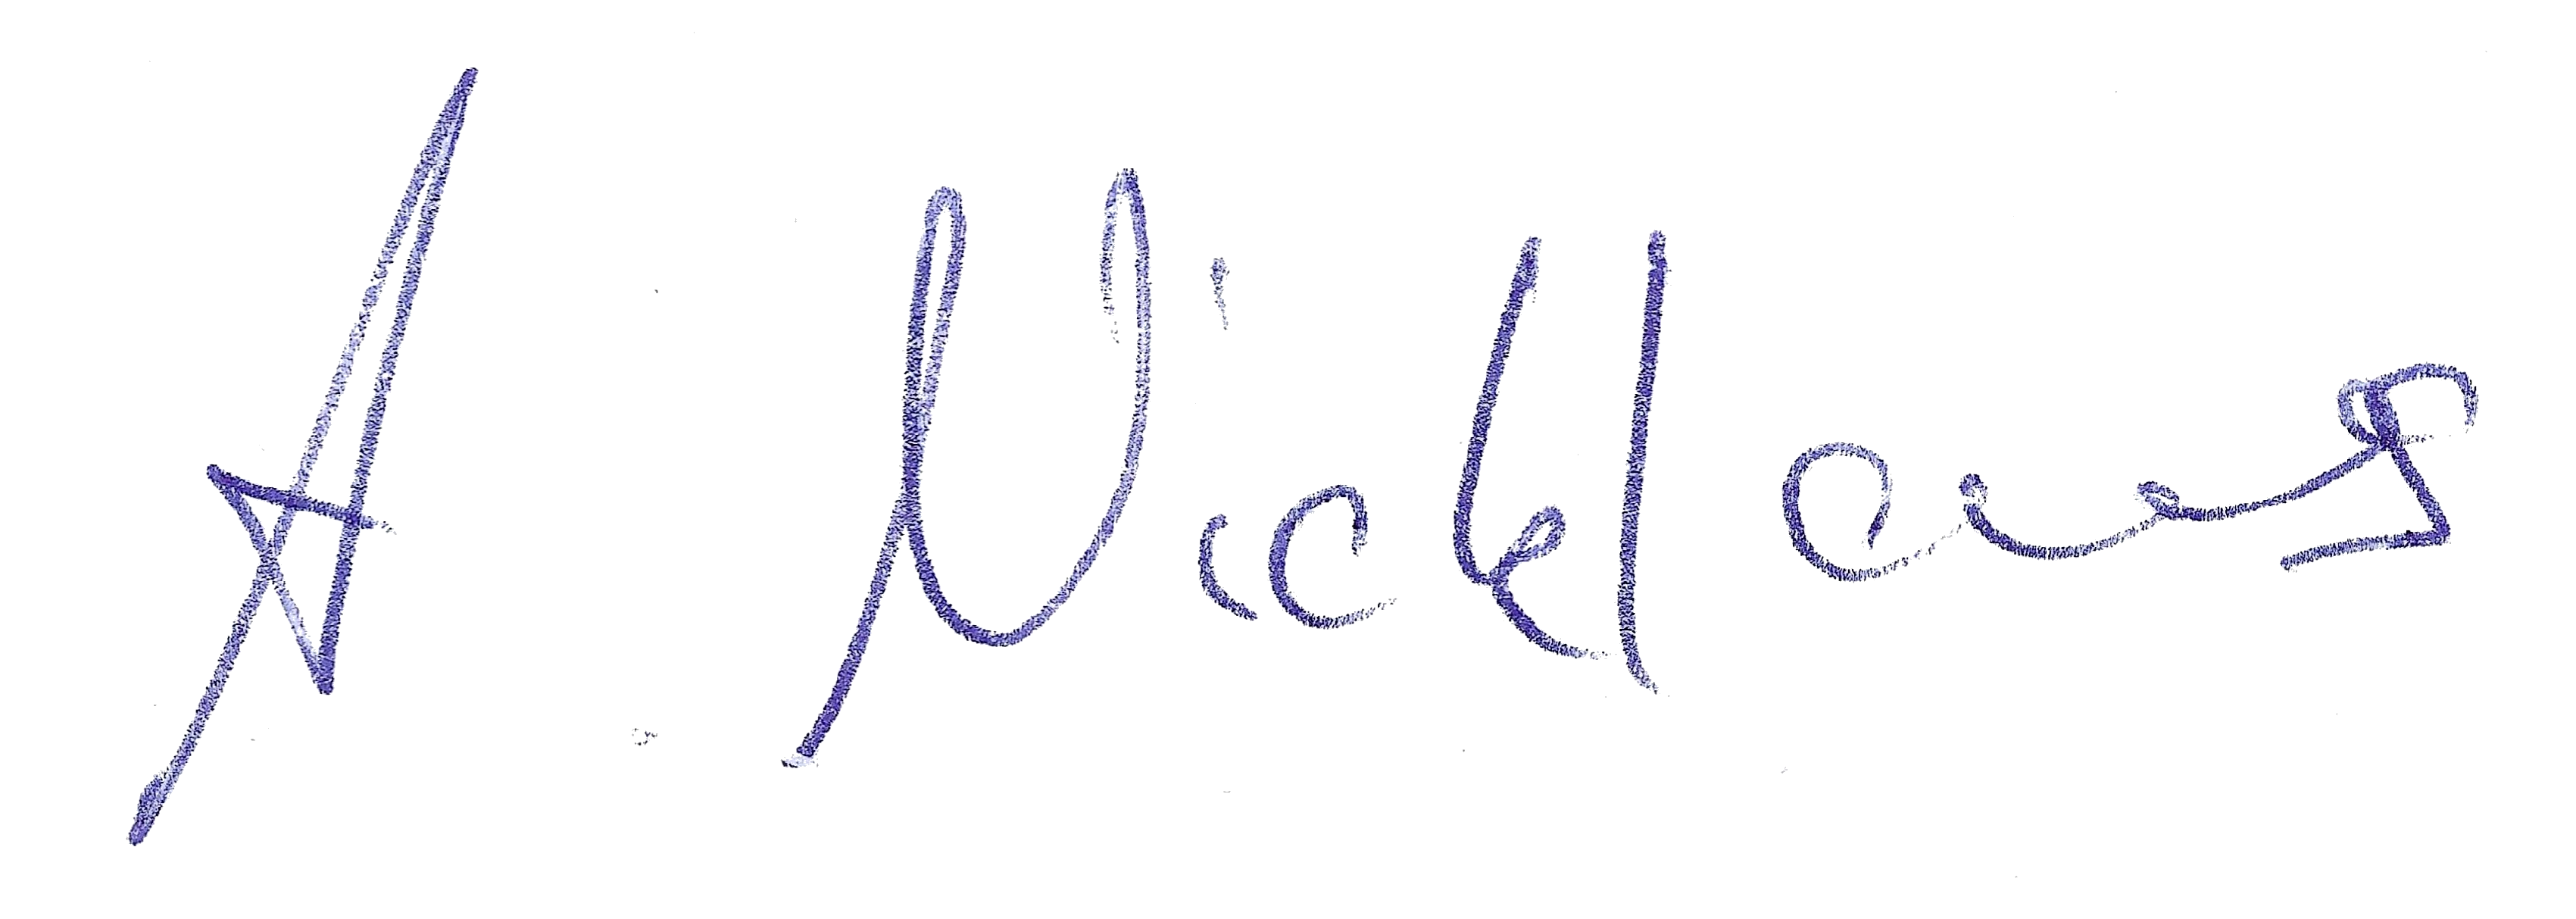
\includegraphics[height=60px]{img/unterschrift.png}
%	\vspace{60px}
	\vspace{10px}
	
	\Author

\pagebreak

\selectlanguage{ngerman}
\begin{abstract}
  Teil eines jeden Webanwendungsprojekts ist die Wahl der Werkzeuge, insbesondere die Wahl des Frameworks für das Entwicklungsteam.
  Leider hat sich diese Diskussion eher zu einer Gefühlsangelegenheit als zu einer sachlichen Angelegenheit entwickelt.
  Diese Arbeit stellt eine Studie über eine beispielhafte Webanwendung vor, die identisch mit sieben gängigen \acrlong{js}-Webentwicklungs-Frameworks erstellt wurde: Angular, Astro, Next.js, Nuxt, React, Svelte und Vue.js.
  Es wird eine Testreihe mit Lighthouse und Playwright vorgeschlagen, um das klassische Laden der Seite, das Laden von \acrlong{js}-Komponenten und die Aktualisierung von \acrlong{js}-Komponenten abzudecken.
  Die Auswertung der Messungen umfasst die Verwendung von zwei neuen abgeleiteten Metriken: die \acrfull{ovcd} und eine loadEventEnd-Metrik, die auf das requestStart-Ereignis der NavigationTiming-Messungen abgestimmt ist.
  Die Ergebnisse zeigen keinen eindeutigen Gesamtvorteil eines einzelnen Entwicklungs-Frameworks, sondern zeigen die Stärken und Schwächen aller getesteten Frameworks auf.
  Die Aktualisierungszeiten von Komponenten weisen Nuxt als das schnellste und Next.js als das langsamste Framework aus.
  Ebenso sind Google Chrome der schnellste und Desktop Safari der langsamste Browser für die Aktualisierung des \acrshort{dom} nach Benutzereingaben.
\end{abstract}

\selectlanguage{english}
\begin{abstract}
  Part of every web application project is the choice of tooling, especially the choice of framework for the development team.
  Unfortunately, this discussion has evolved into a sentiment matter rather than a factual one.
  This thesis presents a study of a single example of a web application created identically with seven mainstream \acrlong{js} web development frameworks: Angular, Astro, Next.js, Nuxt, React, Svelte and Vue.js.
  A testing suite is proposed using Lighthouse and Playwright to cover the classic page load, the load of \acrlong{js} components and the update of \acrlong{js} components.
  The evaluation of the measurements include the usage of two new derivative metrics: the \acrfull{ovcd} and a loadEventEnd metric.
  The results show no clear-cut overall advantage of one single development framework, but outline strengths and weaknesses of all tested frameworks.
  Component update times indicate Nuxt as the fastest and Next.js as the slowest framework for update times.
  Similarly, Google Chrome appears to be the fastest and Desktop Safari the slowest browsers for updating the \acrshort{dom} after user input. 
\end{abstract}

% ?REVIEW: \keywords{framework, web performance, Angular, Astro, Next.js, Nuxt, React, Svelte, Vue.js}

\vfill

\noindent\textbf{Disclaimer:} This thesis has been written with the help of AI tools for translating sources and outlining parts of the written content.
All content has been written or created by the author unless marked otherwise.

\pagebreak

\tableofcontents
\pagebreak

\section{Introduction}\label{sec:introduction}
Throughout the evolution of the world wide web, many changes have disrupted the way websites are created.
From simple file servers run by few selected institutions, simple static web pages and dynamic services like blogs and forums to websites created with the help UI tools and web development frameworks, mainly written in JavaScript, development has changed drastically since its beginning.

Older web pages often lacked features that developers today work with as a matter of course.
Yet their load and rendering most likely would be blazingly fast with today's technological advancements in networking, browser functionalities and user equipment.
Modern websites though are often bigger in size, have a lot more features and are in many respects more complex.
Due to the increased complexity, the mere volume of a website's data has increased, especially with more and more multimedia files.
That in return has increased the demand for better performance on all components of the load and rendering process.
This technological advancement has upped the technological sophistication for development tools as well.
Today's modern web development frameworks support developers with tools to create sites and applications through terminal commands.
They often increase the content-per-line-of-code quota through implicit page generation in contrast to the explicit writing of source code from earlier times.
Many frameworks even feature configuration options for directly hosting the web page.

As the generation process changed from writing code manually to automatically, this implicit page generation undoubtedly increased speed through faster content generation and resulted in a greater development experience for some developers.
Because developer experience varies between different frameworks and some approaches are more intuitive to respective developers, a current trend has evolved for developers to become experts in a single framework rather than many.
This trend lead to a tribal conflict as to which framework is better than others with each tribe being convinced that their framework is the best.
There is no apparent way to objectively determine a \enquote{best framework} in terms of developer experience because it is a subjective criterion.
The performance of a framework as assessed by the developer can be similar or greatly different, depending on the frameworks and the interviewees.

When it comes to user experience and especially the perceived user experience however, there are plentiful collections of metrics and criteria to choose from so as to determine the performance of websites, not frameworks.
The optimization of websites has become a goal during development because it has a real effect on both the ranking of web pages in search engines and the user behaviour.
Both effects create business interests and financial incentives to invest resources into performance optimization \citep{webprophet,effectsofwebpagecontents}.
However, the lack of research on the topic suggests either a consensus for a negligible effect of the development framework on the website's performance or a lack of knowledge of the effect.
Measurements on the effect of the development framework are a major convoluted task simply because the performance of a specific website can be dependent on many other factors such as the user's device, browser, networking hardware or server-side hardware.
The number of possible combinations of factors and their reliability makes it difficult to measure a single performance run with a reliable result.
Every single result is only a small part of a large number of possible performances the same application could achieve with different parameters.
It is therefore perceivable that a \enquote{perfect combination} of hard- and software exists for each framework or in general, but it is currently not possible to find such a combination because the necessary data is missing.

Many modern web tracking services provide data about the user, the user's devices, current page load times and so on.
This data is helpful in determining current poor performances and therefore possible starting points for optimization efforts.
But it gives very little information about recommended actions or recommended choice of frameworks for a redesign of a web application.
Relying on marketing material for choice of frameworks is equally questionable because most modern frameworks claim to be fast, easy to use and performance efficient.
This suggests that each would be a great choice for developers.

In order to find a suitable framework for an application, a set of metrics needs to be at least outlined for comparison.
Many former studies suggest metrics to be relevant for the user experience or \acrlong{seo}.
Content metrics such as word count or presence of meta tags might be important for some performance measurements, but might also have no effect on the user experience.
In contrast, rendering metrics such as page load time or page weight might be ascribed to the framework used during development.

The performance of a framework towards the user can very rarely be compared because there are no publicly available comparisons between exact replicas of web applications built with different frameworks.
Therefore, a comparative study between the same website built with different frameworks is needed to get as close as possible to an exact website replica.
With this data, an informed choice might be made for other projects.

The goals of this thesis are to propose a set of metrics that allow comparing mainstream JavaScript frameworks for web applications, to provide a comparative study between selected frameworks and to create a tool to compare the rendering performance of a page as a whole and of dynamic components within a page.

\section{Related Work}\label{sec:relatedwork}
Methods, measurements and metrics for the performance of web applications have been used and interpreted in many past works.
\cite{webprefetching} propose a list of metrics used for prefetching resources as well as considerations for comparing results and interpreting measurements from a user's perspective.
The considerations for the selection of metrics heavily inspire the selection of metrics in this work.
In addition, they list differences in the underlying base system, the tested workload and key metrics as problems for comparisons between pages and test suites and recommend using latency per page as a key performance metric from the user's point of view.
\cite{sevenpitfalls} and \cite{webprophet} describe relevant non-technical considerations for performance indicators from a user's and stakeholder's perspective.
The effect of user-focused measurements of web page speed is clearly important to a site's effectiveness for objective goals, such as customer lifetime value and user retention \citep{webprophet,sevenpitfalls,effectsofwebpagecontents}.
Also, variants and ambiguities cannot be definitively ruled out as the main source of both bad and good results of performance tests. 

Most previous studies focus on network components and measurements for the evaluation of performance \citep{analyzingfactors,highperformancebrowsernetworking,measuringandmitigatinwebperformance}.
However, these works also take network speeds with a grain of salt because delays such as propagation, transmission, processing and queueing of requests as well as factors like number of requests, network speed and latency heavily influence the results.
Recommended best practices for testing networks from these papers include using multiple clients and server sites.
Additional to these factors, caching is one of the most important strategies for network performance \citep{whatifanalysis,measuringandmitigatinwebperformance}.

\cite{whatifanalysis} separate the page load time into network activities and computation activities by splitting contributions to the load time between rendering jobs.
They also point out the fluctuation of measurements due to the choice of browsers, especially the negative effect of mobile browsers towards load time.
The network activities are described by \cite{webprophet}, \cite{highperformancebrowsernetworking} and \cite{measuringandmitigatinwebperformance}.
In contrast, \cite{effectsofwebpagecontents} point out that the content of a page has a much larger effect on the page load time than the client or network conditions. 

Work on client optimization efforts include the effect of page load time on the user, selection strategies for tested pages and factors for the customers' perception of response time.
According to \cite{webprophet}, a delay of 100 ms results in a sales loss of 1 \% and 500 ms delay lead to up to 20 \% sales loss.
A delay of one second, decreases the customer satisfaction by 16 \% \citep{effectsofwebpagecontents}.
The customers' expectation in most cases are availability and response time and their perception is based on many factors \citep{loadtestingofwebsites}.
The choice of tested pages is a difficult one because no usage data is available at build time and sitemaps only give hints about the pages' content and pages that are important to the site's effectiveness \citep{onlandingandinternalwebpages}. 

Lastly, \cite{integratedapproach} gives guidelines to designing a web performance testing tool and points out attributes of good benchmark.
Tests are based on stakeholders' expectations for load times and web pages are classified based on the complexity and interactivity of their content.
This classification strategy is also applied in this work.
Results show that the page load time is pivotal for the bail out percentage of users.

\section{Setup of the application and test environment}\label{sec:design}

Whereas the following chapters cover the implementation of testing and evaluation of results, this section introduces the conceptual design of the comparative study.
The goals of and requirements for the example application, the differences and choices for the hosting environments for testing and the tools for testing as well as selected metrics are described here.

\subsection{Example Web Application}\label{subsec:exampleapplication}
% What goals does should the example app fulfil?
% What parts does the example app consist of?
% What requirements does the app cover?
%
% 1. App Idea
% 2. Pages
% 3. Page intention & type
% 4. Multimedia Files & Video Autoplay
% 
% MOSCOW-Analyse
% UML-Diagramme: Services, Pages, Entities

The example application for the study is designed to be a benchmark application for testing.
The following goals were considered during the design process:

\begin{enumerate}
  \item \textbf{Page types}: With the goal of covering most kinds of web pages, three types were identified based on the time of data loading.\label{enum:pagetypes}
  These types differ in timing at which the \acrshort{dom} content is loaded or updated.
  The definition of a finished load or update for this work is that the linking of resources does constitute a finished load or update of the web page regardless of the load time of said resource on the condition that any linked resource does not update the \acrshort{dom} in any way.
  If a resource does mutate the \acrshort{dom}, then the load or update is considered not finished.
  \begin{enumerate}
    \item Static pages are web pages which do not change their content after the initial response from the web server.
    The initial \acrshort{html} document already is the only resource that is necessary to create a complete \acrshort{dom}.
    If inline scripts update the DOM, they are considered external resources.
    \item Delayed pages do not have a complete \acrshort{dom} after loading and parsing the initial \acrshort{html} document.
    Some data or content is loaded and inserted (or removed) into the \acrshort{dom} after the initial render.
    The time of these updates can be any time after the initial render, but the execution of code or start of request for the resource that is responsible for the update has to be directly or indirectly triggered by the content of the initial \acrshort{dom} or \acrshort{html} document.
    \item Dynamic pages can be updated or update themselves by events that are not triggered by the content of the initial \acrshort{dom} or \acrshort{html} document.
    These events can either be triggered by user interaction or other events such as websocket messages.
    The time of such updates is by their nature not predictable.
    Dynamic pages are either static or delayed with additional opportunities for updates.
  \end{enumerate}
  This list is created with the knowledge that frameworks or other technologies such as caching may move a web page from one type to another.

  \item \textbf{Modern Development Practices}: The example application should contain modern development practices that do project onto the \acrshort{dom}.
  Practices that have no effect on either the projection of data or user interactions, such as coding styles or project management, are considered to have no effect on the performance of the page.
  
  \begin{enumerate}
    \item Components: All pages of the app have to consist of components that encapsulate reproducible \acrshort{html} snippets and may project data onto the \acrshort{dom}.
    \item List iteration: Because iterating long lists may decrease performance noticeably, some components or pages should implement list iteration.
    \item String interpolation: Although it is not considered a performance issue before testing, string interpolation is prevalent in all modern frameworks known to the author.
    \item Services: \label{enum:services} Separation of functions in services is a wide spread practice to reduce code duplicates and easy refactoring.
    In this case, services also allow to intentionally implement delays for testing purposes.
  \end{enumerate}
  
  \item \textbf{\acrshort{css}}: Even though the usage of \acrshort{css} can in no way be considered a modern practice, it is still used on effectively every web page.
  Additionally, stylesheets are considered render-blocking resources that impact performance negatively \citep{renderblocking,eliminateRenderBlocking}.
  For this purpose, \acrshort{css} shall be included in all pages and components.
  
  \item \textbf{Rendering time}: In addition to the page type depending on the time of data load, the time of composing the \acrshort{dom} is dependent on the content availability.
  For this thesis, three different types are considered:
  \begin{enumerate}
    \item \acrfull{csr}: The initial request gets a response with a mostly empty \acrshort{html} document (\enquote{skeleton}) except linked \acrshort{css} and \acrshort{js} resources which after loading, parsing and executing update the \acrshort{dom}.
    \item \acrfull{ssr}: Updates that happen after receiving the skeleton through \acrshort{js} code execution on \acrshort{csr} happen before the initial request is responded to on the web server.
    The initial \acrshort{html} document is filled and no longer a skeleton with \acrshort{ssr}.
    Therefore, it has greater byte size.
    \acrlong{ssr} requires an \enquote{active} front-end server rather than only a file server to execute code.
    \item Prerendering: Rendering happens during build time of the application.
    This increases the build time and the byte size of the initial \acrshort{html} document, but only a file server is needed for hosting.
  \end{enumerate}

  \item \textbf{Multimedia}: Most of network load and therefore network delay is caused by multimedia files.
  Although compression has gotten better over time, the byte size taken up by multimedia files of a web page has gotten larger over the last years \citep{pageweightreport}.
  Therefore, size optimization of image and video files is considered a major part of performance optimization and a great potential for a performance increase by the used framework.

\end{enumerate}

Based on these considerations, the application \enquote{NotInstagram} was designed as a comparable example application.
It is heavily inspired by the Android app Instagram and a partial reproduction of its app design \citep{instagram}.
\enquote{NotInstagram} consists of four pages (see figure \ref{fig:screenshots}).
\ref{subfig:index} shows the design of the Feed page.
It is the start page of the app and contains 4 parts: the header, the profile list, the post list and a footer.
Each item of the Feed page is to be implemented as its own component or components.
The plus icon in the header links to the Create page, the footer links to the About page and every instance of a profile picture and profile name links to a Profile page.
The latter contains profile information including a profile picture, name, user handle / ID, profile creation time, caption and a grid of all the user's posts (see figure \ref{subfig:user}).
The profile component encapsulates all \acrshort{html} elements of that page except the header containing the app logo and X icon, which both link back to the Feed page.
Both the Feed page and the Profile page are generally expected to classify as delayed pages, because the content of profile and posts lists can only be loaded after the page load.

The Create page (see figure \ref{subfig:create}) has three parts.
The header contains the app's logo and an X icon linking to the feed.
A form with three input elements and a \verb|<button>| element allows for the input of a multimedia source (image or video) and a text caption.
The multimedia source can either be a \acrshort{url} or a selection from a list of preuploaded files.
The post caption is a pure text input.
The lower part of the page is the post preview, in which some predefined information such as user profile and the user inputs are combined.
As such, the Profile page is a static page until the user uses the creation form, at which point it has to be considered a dynamic page.
The About page (see figure \ref{subfig:about}) is designed to statically display information about the application.
It is a static page because no content is loaded after a delay and no user inputs are possible.

With these pages all \hyperref[enum:pagetypes]{page types} are covered for testing.
The About page and Create page are static, whereas the Feed page and Profile page are partly static (header and footer), but mostly delayed.
The Create page is the only page with dynamic content.

\begin{figure}[ht!]
  \begin{subfigure}{0.49\linewidth}
    \begin{center}
      
\includegraphics[width=\linewidth, height=0.3\textheight, keepaspectratio,frame]{img/ig-clone/Feed.png}
    \end{center}
    \caption{Feed page (/)}\label{subfig:index}
  \end{subfigure}
  \begin{subfigure}{0.49\linewidth}
    \begin{center}
      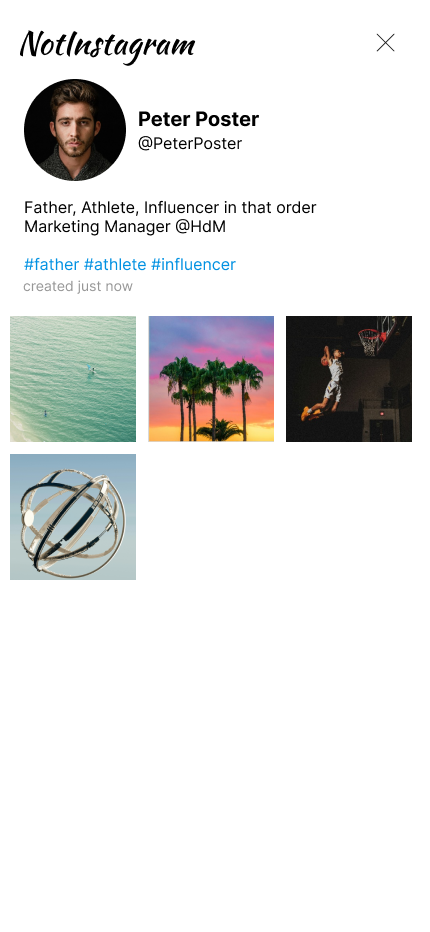
\includegraphics[width=\linewidth, height=0.3\textheight, keepaspectratio,frame]{img/ig-clone/Profil.png}
    \end{center}
    \caption{Profile page (/user/@PeterPoster)}\label{subfig:user}
  \end{subfigure}
  \begin{subfigure}{0.49\linewidth}
    \begin{center}
      
\includegraphics[width=\linewidth, height=0.3\textheight, keepaspectratio,frame]{img/ig-clone/Beitrag erstellen.png}
    \end{center}
    \caption{Create page (/create)}\label{subfig:create}
  \end{subfigure}
  \begin{subfigure}{0.49\linewidth}
    \begin{center}
      
\includegraphics[width=\linewidth, height=0.3\textheight, keepaspectratio,frame]{img/ig-clone/Informationsseite.png}
    \end{center}
    \caption{About page (/about)}\label{subfig:about}
  \end{subfigure}
  \caption{Screenshots of the NotInstagram application's pages (path in parentheses)}\label{fig:screenshots}
\end{figure}

The data fetching and loading is designed to be implemented as \hyperref[enum:services]{services}.
For NotInstagram, two different services are needed.
The PostService is a service for all components to query posts.
The method \verb|getAll()| returns a list of all posts by all users and \verb|getByUserHandle(handle)| returns the same list filtered by those posted by a user with the handle equal to the function parameter.
ProfileService is a service to query user profiles.
It has the same two methods which return all user profiles and only one user profile respectively.
Services are designed asynchronous, but the data is not queried from a server external to the browser, but hard coded.
This design decision is based on the premise that delay can be coded into or out of asynchronous functions to mimic network delay for testing purposes if necessary.

Figure \ref{fig:uml} describes the usage of components and services within page views.
It displays the four pages of NotInstagram, the two services and 15 components.
Seven of those components are icon components.
Those components serve as wrappers for \acrshort{svg}s to ensure their correct scale and style.
\verb|XIcon| poses an exception to the design as it is a wrapper for a \verb|PlusIcon| component rotated by 45°.
The colored arrows show the usage of one of the services.
Both the Feed page and the Profile Page use the services to load data.
For the Feed page, both \verb|PostService.getAll()| and \verb|ProfileServices.getAll()| are needed to pass the data to \verb|PostList| and \verb|ProfileList|.
Notably, each \verb|Post| component accesses the ProfileService again, to get the profile image and name for its headline, even if the information is available in a parent or grandparent component.
Figure \ref{fig:classes} displays the connections between post and profile object instances.
The member \verb|userhandle| of a post references the member \verb|handle| of a user profile.
The Profile page needs access to the services in order to get the information of the requested profile and a list of posts from the \verb|getByUserHandle| methods to pass into the \verb|Profile| component.
\verb|LogoHeader|, \verb|NotInstagramLogo| and \verb|InfoBlock| are not data-presenting components, but rather styling components.
Their only function is styling text or projecting \acrshort{html} elements with \acrshort{css} information.

\begin{figure}
  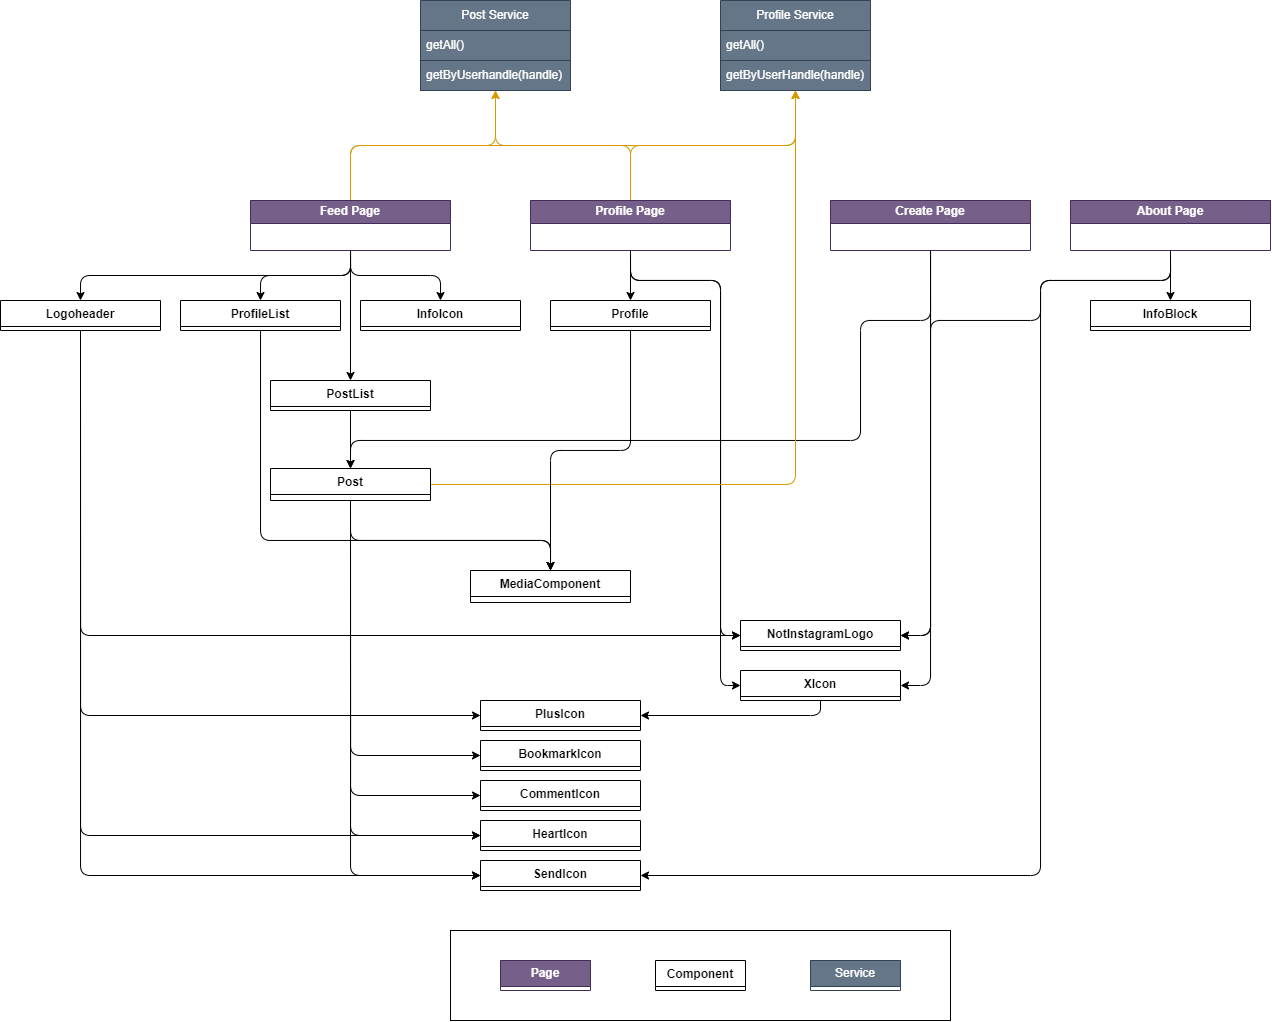
\includegraphics[width=\linewidth]{diagrams/uml.png}
  \caption{Pages, components and services of the NotInstagram application}\label{fig:uml}
\end{figure}
\begin{figure}
  \begin{center}
    
\includegraphics[width=0.5\linewidth]{diagrams/entities.png}
  \end{center}
  \caption{Classes used by the NotInstagram services}\label{fig:classes}
\end{figure}

In contrast, the \verb|MediaComponent| is designed as a way to allow both internal and external images and video sources.
It is used by \verb|ProfileList|, \verb|Post| and \verb|Profile| to display posts and profile images.
Its main goal is to decide - based on the passed source string - how to project the multimedia file onto the \acrshort{dom}.
The component accepts source strings for images and videos, differentiated by the string's ending and therefore the file's extension.
If it is a local image, namely an image that was available for optimization at build time, the best available form of optimized \verb|<img>| tag should be used.
For external image links starting with \enquote{http://} or \enquote{https://} a less optimized or unoptimized \verb|<img>| tag shall be inserted into the \acrshort{dom}.
For videos, any source string is to be projected onto a \verb|<source>| tag with identical \verb|<video>| wrapper.

The application refers to local images, which can possibly be optimized, and external images, which cannot be optimized.
The reason for this is the assumption for this project that optimizing multimedia files uploaded by a user and referencing them in a manner suitable for this application is not suitable for this study.
Rather, the better alternative for serving the use case of the application would be a dedicated server for encoding, decoding and generally optimizing multimedia files.
Since this solution would be independent from the front-end framework's performance and it would outgrow the scope of this work, a distinction is only made between static images, called local images here, and external images with full \acrshort{url}s.

\subsection{Choice of web frameworks}
% Which frameworks were chosen to test?
% Why were these frameworks chosen?
% Which frameworks/tools were considered

% \addcontentsline{toc}{subsubsection}{Angular}
% \addcontentsline{toc}{subsubsection}{Astro}
% \addcontentsline{toc}{subsubsection}{Next.js}
% \addcontentsline{toc}{subsubsection}{Nuxt}
% \addcontentsline{toc}{subsubsection}{React}
% \addcontentsline{toc}{subsubsection}{Svelte}
% \addcontentsline{toc}{subsubsection}{Vue.js}

\begin{table}[b]
  \begin{center}
    \begin{tabular}[h]{|l|c|c|c|}
      \hline
      ~                 & \textbf{\acrshort{csr}} & \textbf{\acrshort{ssr}} & \textbf{Previous Experience}  \\ \hline
      \textbf{Angular}  & yes                     & no                      & yes                           \\ \hline
      \textbf{Astro}    & yes                     & yes                     & yes                           \\ \hline
      \textbf{Next.js}  & no                      & yes                     & no                            \\ \hline
      \textbf{Nuxt}     & yes (generate)          & yes (build)             & no                            \\ \hline
      \textbf{React}    & yes                     & no                      & yes                           \\ \hline
      \textbf{Svelte}   & yes                     & no                      & no                            \\ \hline
      \textbf{Vue.js}   & yes                     & no                      & yes                           \\ \hline
    \end{tabular}
  \end{center}
  \caption{List of selected frameworks. Items with both \acrfull{csr} and \acrfull{ssr} render some pages or components upon request, but also require \acrfull{csr}. Previous Experience refers to the author's experience in developing web applications with the framework.}
  \label{tab:frameworks}
\end{table}

The choice of tested frameworks for this study is the choice for which frameworks the application will be implemented in and tested.
The requirements for this selection are twofold.
The application has to be implementable as designed above with the framework without the use of any other non-native tool to the framework or any tool that was not officially intended to be used in combination by the developers of the primary framework.
Additionally, the application must be implementable in JavaScript.
This requirement includes TypeScript frameworks because it is possible to use JavaScript in TypeScript applications \citep{typescript}.
Ease of use and developer experience should explicitly not influence the selection process because it is not part of the performance of the resulting website.

Because research revealed in early stages of the study that many frameworks fulfill those requirements, the long list of candidates had to be sorted.
The deciding factor for this selection was usage, awareness of and positive sentiment towards tools among developers because the evaluation of mainstream and general-purpose frameworks appear more valuable than lesser known or specialised tools.
A ranking of the most-used JavaScript front-end frameworks of 2023 \citep{stateOfJs2023} lists the four frameworks with the most developers who have used it before: React (84 \%), Vue.js (50 \%), Angular (45 \%) and Svelte (25 \%).
In addition, Astro was chosen for its especially high awareness among the category \enquote{other front-end tools} (30 \%), as well as its usage (19 \%) and interest (62 \%) in the category \enquote{meta-frameworks}.
From the last category of tools, two other frameworks were selected: Next.js and Nuxt.
Both tools are highly-used frameworks and have the appearance and goal of improving on React and Vue.js, respectively.
For this reason, they are interesting choices for this study.
All selected frameworks fulfill the requirements.
The application is implementable with all frameworks or intended addition of tools.
Next.js and Nuxt require the usage of React or Vue.js tools and dynamic components cannot be written in pure Astro \citep{AstroIslands}.
Astro intends the usage of other frameworks to implement so-called \enquote{Islands}.
For those components, React was chosen for its top usage rate.

Other frameworks were also considered for selection.
Solid and Qwik seemed fitting candidates in this study because of high interest among developers without experience with the frameworks and apparent potential for fast performance of their end product.
Additionally, from the ranking of most-used front-end frameworks Preact was at least considered with a usage percentage of 13 \%.
Ultimately, all three were not chosen because of negative sentiment or low usage among developers that do have experience with these frameworks.
This concludes the framework selection for this study.
Table \ref{tab:frameworks} list the selection and categorizes them into groups with and without \acrshort{csr} and \acrshort{ssr}.
It also states whether the author of this thesis and developer for the application had any previous experience working with the framework.
This information is important for the unintended performance optimizations and could later be used for interpretation of the frameworks performance measurements.

To summarize some comparisons between frameworks or groups of frameworks, the most appealing for the evaluation are the following:

\begin{enumerate}
  \item \textbf{\acrshort{csr} - \acrshort{ssr}}: Before testing, differences between \acrshort{csr} and prerendered pages are expected, but the metrics and amount of differences are probable subjects of interest.
  Because there is no perceivable difference between prerendered pages and server-side rendered pages from a client perspective, they are grouped together in this context.
  \item \textbf{Angular - React - Vue.js}: Because these \acrshort{csr} frameworks have been competing for eight years at this point and they are still the most famous front-end frameworks \citep{stateOfJs2023}, the comparison of these frameworks is relevant for this study.
  \item \textbf{Nuxt - Vue.js}: As a next generation of the Vue.js framework, the actual performance increase of Nuxt is interesting for developers.
  \item \textbf{Next.js - React}: Same as above in relation to React
  \item \textbf{Vue-based - React-based}: Because a direct comparison of frameworks based on React and based on Vue.js is possible with multiple candidates, a difference in performance is an actual relevant factor for the choice between the two ecosystems.
  \item \textbf{Svelte - Astro}: As the most recent popular frameworks in the selection of frameworks, Astro and Svelte have the potential to both outdo their contenders and outdo each other.
  This comparison is most interesting for fans of new tools and the development teams of the frameworks themselves.
\end{enumerate}

% REVIEW: introduce the frameworks
% * irgendwie fehlt noch etwas:
% - Definition des Wortes framework (Grundwissen)
% - Einführung in Frameworks (Grundwissen)
% - Welche Art von Framework ist nicht abgedeckt? (Faß ohne Boden)

\subsection{Hosting Environments}\label{subsec:hostingenvironments}
% Based on former work, networking plays a vital role in performance and load times
% 
% What exactly should be tested?
% What requirements do the environments have to cover?
% What properties should be considered for the environments?
% 
% 1. Vercel
%    1. Reason
%    2. Problems
%    3. Solutions
% 2. Local
%    1. Reason (Network delay)
%    2. Problems

After designing the application, the next step in the study process was to decide where the application is to be hosted for testing.
Network delay is a great part of render delay and performance issues \citep{highperformancebrowsernetworking} because loading files in sequence will block rendering if parsing documents and executing code is dependent on network requests.
The request delay is based on the speed of the web server, the network speed and the size of the generated file, request and response.
Therefore the time needed for fulfilling network requests should be considered in the choice of hosting environment or service.

\begin{figure}[h]
  \begin{center}
    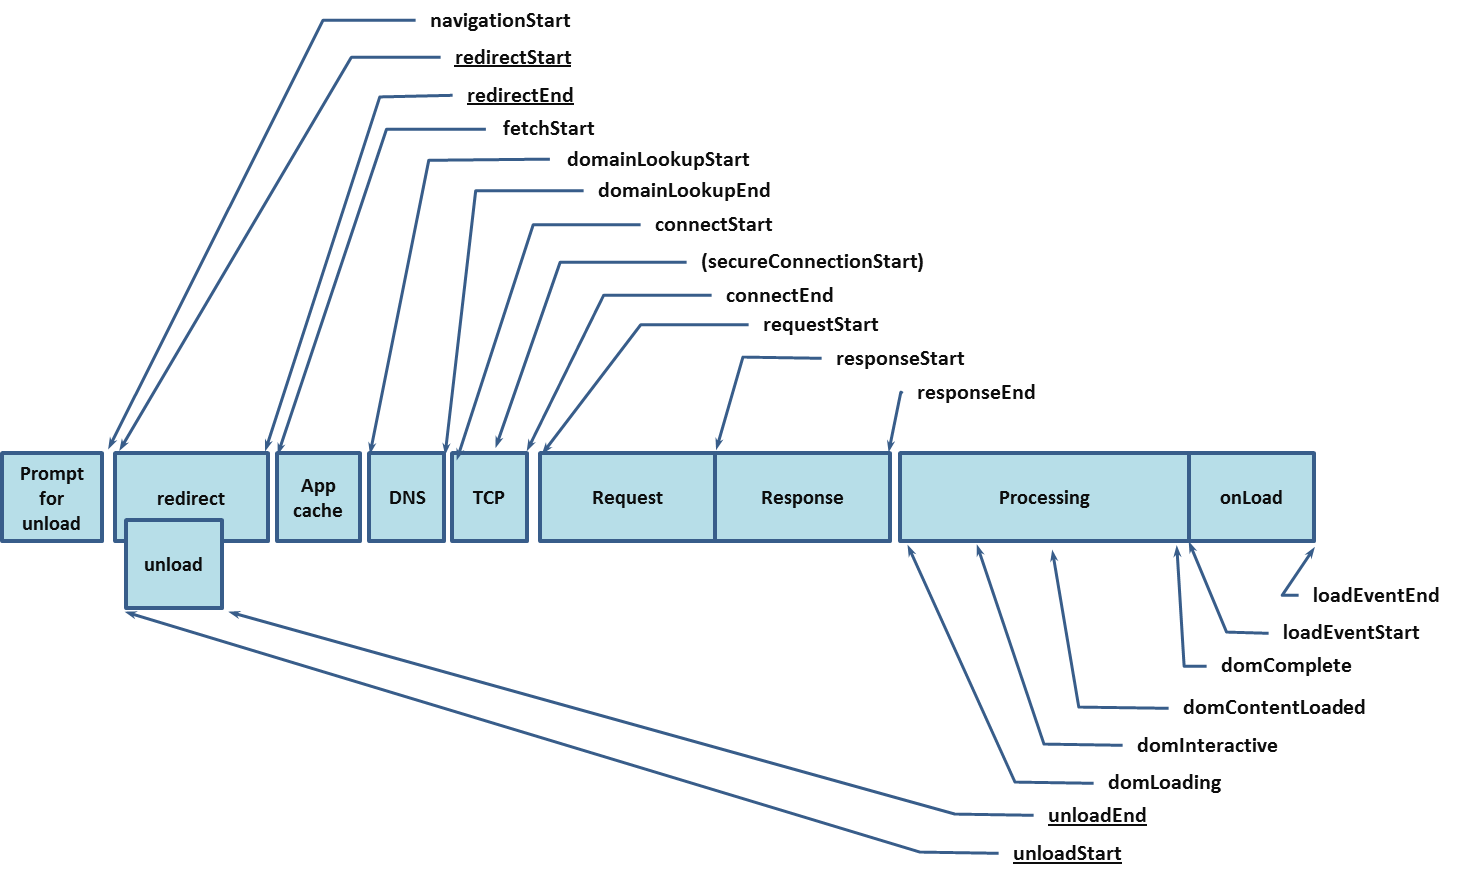
\includegraphics[width=\linewidth]{img/request-timing.png}
  \end{center}
  \caption{Timing attributes defined by the PerformanceTiming interface and the PerformanceNavigation interface \citep{navigationTimings}}\label{fig:timing}
\end{figure}


Figure \ref{fig:timing} illustrates how a slow network may delay the rendering process of a web page.
The tests for this study shall cover real-world hosting using a publicly available service and local hosting to test the network delay and test the application without interference of network speeds.
Additionally, tests can not be done only on local servers because tests shall include timings before responseEnd.
Requirements for the distant hosting environment or service are threefold.
The service shall have \enquote{active server capabilities}, meaning capabilities that exceed pure static fileserver functions for \acrlong{ssr} and similar functionalities.
Furthermore, it is required to be a widely used hosting service to ensure the real-world applicability of the study.
Since this requirement is not clearly definable, it is considered a guideline.
Lastly, to be applicable for small projects as well as established larger websites the service chosen for the study is required to support free usage and integration into a \acrfull{cicd} pipeline because it is a widely used development practice.
As such, the integration is important to require the least possible manual configuration for hosting the application because this study is not supposed to be about the configurability.
Rather, the study shall focus on the "out of the box" performance of the frameworks.
Continuing with that sentiment, the optimization and therefore configuration of the hosting environment is not part of this work.
This is the methodology for answering the question: With which framework do developers get the best performance for their web applications without spending much or any time with optimization and configuration?

% \begin{mylist}
%   \begin{itemize}
%     \item Vercel
%     \item Localhost
%   \end{itemize}
%   \caption{Chosen hosting environments}
% \end{mylist}

\subsubsection{Vercel}
Based on these considerations and personal experience with the service of the author previously to this project, Vercel was chosen for hosting the application.
Vercel supports predefined configurations and automatic recognition of all frameworks chosen for this study.
Also, Vercel projects integrate seamlessly into a \acrshort{cicd} pipeline based on its integration with GitHub.
A GitHub repository was created for each framework and connected to a Vercel project.
During initialization of the Vercel projects and first preliminary tests, one problem with Vercel's free account quickly became apparent:
The bandwidth limitation of 100GB per month and account was reached after two weeks of testing unoptimized and unfinished versions of the applications with large image and video files.
Because no information was found on the effect of a reached limit, the account was deemed dead for the month.
The solution to this problem was the creation a second free Vercel account and the plan to create another account every time the limit would be reached in the future, which it did not.

\subsubsection{Localhost}\label{subsubsec:localhost}
\begin{table}[h]
  \begin{center}
    \begin{tabular}[h]{| l | l | l |}
      \hline
      \textbf{Framework} & \textbf{Build Command} & \textbf{Host Command} \\ \hline
      Angular & \verb|ng build| & \verb|serve| \\ \hline
      Astro & \verb|astro build| & \verb|astro preview| \\ \hline
      Next.js & \verb|next build| & \verb|next start| \\ \hline
      Nuxt & \verb|nuxt build| & \verb|nuxt preview| \\
      & \verb|nuxt generate| & \verb|nuxt preview| \\ \hline
      React & \verb|react-scripts build| & \verb|serve| \\ \hline
      Svelte & \verb|vite build| & \verb|vite preview| \\ \hline
      Vue.js & \verb|vite build| & \verb|serve| \\ \hline
    \end{tabular}
  \end{center}
  \caption{Build and host command for each used framework as used for testing the applications hosted locally}\label{tab:hostCommands}
\end{table}

The second hosting solution for this study is hosting the application locally on the testing machine.
The client device in question is a HP Envy x360 Convertible 15-eu0xxx with an AMD Ryzen 5 5500U processor and 16GB RAM.
The operating system on the device is Windows 11 Home (Version 10.0.22631) during testing.
This environment ensures minimal network load times and eliminates every other connected delay such as resolving domain names.
If the framework supports a \enquote{preview} mode, it was used for hosting the application.
Otherwise, the application would be build and hosted using the \verb|serve| command or the active server would be started with \verb|node <filename>|.
If neither of the two options would be available, the \enquote{dev} mode of the application would be used and tested.
Table \ref{tab:hostCommands} lists the used commands for building and starting the webserver per framework.

\subsection{Performance Metrics}\label{subsec:performancemetrics}
% What metrics can be measured?
% What metrics should be used?
% What metrics will be used?
% 
% 1. Lighthouse performance
% 2. Page weight
% 3. Largest/First Contentful/Meaningful Paint
% 4. TTFB/TTI/SpeedIndex

Slow load time and reactivity of a web page and its user interface decreases user retention and continuing user actions over time independently from the content \citep{webprophet,effectsofwebpagecontents}.
The \enquote{reaction time} is interpreted in three separate ways for this study: The page load time, meaning the time from navigation start to \acrshort{dom} mutation, the time from a state change, e.g. data query end, to \acrshort{dom} mutation, here called component load time, and the time between a user input to finished \acrshort{dom} mutation, called component update time for this study.
Nearly most of these times can be combined from or described using navigation events (see figure \ref{fig:timing}).
These timing categories are not exclusive, but measurements for these time categories do overlap (see table \ref{tab:metriccategories}).

Naturally, other metrics than the navigation timings were also considered.
From the list of measurements in Lighthouse reports (see chapter \ref{subsec:testingtools}), sublists with relevant metrics were created to properly represent the time measurements of the described render sections and DOM mutation events.
These reports cover the initial load of a page and visual content presentation after initial load.
None of the Lighthouse metrics cover the time of \acrshort{dom} mutations after user input events.
Therefore, yet additional measurements have to be considered to describe the performance of mutations.
To this end, some self-written code is injected through Playwright (see chapter \ref{subsec:testingtools}) to measure the time of updates to the \acrshort{dom}.
The following sections describe which measurements are needed for each render section in detail.

\begin{table}[h]
  \begin{center}
    \begin{tabular}[h]{|l|l|l|}
      \hline
      \multicolumn{1}{|l|}{\textbf{Page}}       & \multicolumn{2}{c|}{\textbf{Component}}     \\ \hline
      \multicolumn{1}{|l|}{\textbf{Load Time}}  & \textbf{Load Time}  & \textbf{Update Time}  \\ \hline
      TBW                                       & OLVC                &                       \\ \hline
      TTFB                                      & OFVC                &                       \\ \hline
      \multicolumn{2}{|c|}{TTI}                                       &                       \\ \hline
      \multicolumn{2}{|c|}{TBT}                                       &                       \\ \hline
      \multicolumn{2}{|c|}{LoadEventEnd}                              &                       \\ \hline
      DomContentLoaded                          & \multicolumn{2}{c|}{DOM Mutation Times}     \\ \hline
      LVC                                       &                               &             \\ \hline
      LCP                                       &                               &             \\ \hline
    \end{tabular}
  \end{center}
  \caption{Assignment of metrics to the metric categories}
  \label{tab:metriccategories}
\end{table}

\subsubsection{Page Load Times}\label{subsubsec:pageloadtimes}

In the context of this study, the first contact point for a user to a web page is considered to be the first page load or initial page load.
Within the initial load, the user's main expectations and goals are assumed to be finding a page with the wanted information or input rather than finding the information itself.
As a result, the aim of the client's browser and render engine for this first time frame, called \enquote{page load} here, is to both parse \acrshort{html} and project the content of the page onto the \acrshort{dom}.
In order to focus on this time frame, these metrics describe the application's performance.

\begin{itemize}
  \item \textbf{\acrfull{tbw}}: The total size of files or response body directly increases either the App Cache time between \verb|fetchStart| and \verb|domLoading| or \verb|domContentLoaded| if the resource can be cached in the client, or the response time between \verb|responseStart| and \verb|responseEnd| otherwise.
  \item \textbf{\acrfull{ttfb}}: The time between \verb|navigationStart| and \verb|responseStart|.
  Most of the network delay can be described by the \acrshort{ttfb}.
  Often inaccurately paraphrased as \enquote{ping}.
  \item \textbf{\acrfull{tti}}: The time until the page can be interactive is described by the \acrshort{dom}'s loading state.
  Is is defined through navigation events as the time between \verb|navigationStart| and \verb|domInteractive|.
  Notably, the timing of \verb|domInteractive| is not reliable because a \acrshort{dom} may become interactive, but the browser may not be interactive yet.
  Additionally, resources may still be loading.
  For example, a \acrshort{dom} from a \acrshort{html} skeleton may be \enquote{interactive} after a few milliseconds, but no content may be rendered for the user to see, because \acrshort{csr} code is still loading \citep{htmlLivingStandard}.
  \item \textbf{DomContentLoaded}: Similar to \acrshort{tti}, DomContentLoaded measures the time between \verb|navigationStart| and \verb|domContentLoaded|.
  At this point in time, \enquote{all subresources apart from async script elements have loaded} \citep{htmlLivingStandard}.
  A large difference between \acrshort{ttfb} and DomContentLoaded indicates a great size or at least long load time of subresources.
  \item \textbf{LoadEventEnd}: Total time spent immediately after initial load of a page until the \acrshort{dom}'s onload event is finished.
  This is the time from \\
  \verb|navigationStart| to \verb|loadEventEnd|.
  The time represents both the capability of the used framework to optimize the usage of a client's and network's resources on initial load and the prioritization of JavaScript execution by splitting not immediately needed code into async scripts.
  Therefore, it is a combined indicator for the code performance and general optimization.
  \item \textbf{\acrfull{tbt}}: The \acrshort{tbt} is the total time spent by a browser with parsing and optionally resources that block the rendering process from finishing.
  This includes stylesheets and scripts without the \verb|async| or \verb|defer| tag.
  The metric directly represents the time before the browser can fulfill the user's goal on initial load.
  \item \textbf{\acrfull{olvc}}: This is the time from \\
  \verb|navigationStart| until the last visual change above the fold, meaning within the viewport of the user.
  Metrics with the \enquote{observed} are not throttled by the test tool.
  \item \textbf{\acrfull{lcp}}: The \acrshort{lcp} is the time between navigation to the page and the time of rendering for the visually largest text or image element in the user's viewport \citep{lcpDocumentation}.
  Optimization of this metric requires an understanding of the page's content and element size within the viewport.
\end{itemize}

From this list of relevant metrics, some expectations can be formulated before testing for them.
\begin{enumerate}
  \item \acrshort{tbt} is most likely longer with \acrshort{csr} frameworks because the code execution filling the \acrshort{html} skeleton takes some time that is not necessary in clients with \acrshort{ssr} and Prerendered pages.
  On delayed pages this difference is expected to be very slight or nonexistent.
  \item The \acrshort{lcp} probably will not differ across frameworks, but naturally across pages.
  In contrast, if a framework does create a faster result for its \acrshort{lcp}, it is expected to be a \acrshort{ssr} or Prerendering framework because of its expected shorter \acrshort{tbt}.
  \item \acrshort{csr} frameworks differ from \acrshort{ssr} and Prerendering frameworks by \acrlong{tbw} similar to \acrlong{lcp}.
  Although the \acrshort{html} document is much slimmer with \acrshort{csr}, the \acrshort{js} files are expected to be equally larger than server-side rendered and prerendered pages.
  It is probably nearly equal in sum because the byte size of the page is likely mostly made up from multimedia files such as images and videos. 
  \item The selected frameworks should be inversely separable into groups by the \acrlong{ttfb}.
  Most likely \acrshort{csr} and Prerendering frameworks will be faster for this metric because the web server can serve as a static fileserver and does not have to execute any additional code.
  \item Because \acrshort{csr} pages consist of only nearly empty \acrshort{html} skeletons and links to \acrshort{js} and \acrshort{css} files, the \acrshort{tti} is expected to be much faster for \acrshort{csr} pages.
  \item The timing of the \verb|loadEventEnd| is not clearly predictable before testing.
  The only expectation is that newer frameworks perform better in this metric simply because they are newer and are expected to make optimizations that go into a faster parsing and rendering of a web page.
\end{enumerate}
  
\subsubsection{Component Load Times}\label{subsubsec:componentloadtimes}
% Measuring JS-dependent parts of the webpage
% 
% 1. Dom Updates with MutationObserver
% 2. Problems with MutationObservers and Playwright

As a second category of relevant metrics, measurements for the separation of the app into components are grouped together.
This category is designed to reflect the performance of the \acrlong{js} that was generated by the framework.
This stands in contrast to how much content can be rendered by the time of \verb|responseEnd|.
To this end, only measurements after \verb|responseEnd| can be taken into consideration.
Each mutation from the initial \acrshort{dom} has to be interpreted as an update to a component.
The following metrics are part of this category.

\begin{itemize}
  \item \textbf{LoadEventEnd}: as explained in section \ref{subsubsec:pageloadtimes}
  \item \textbf{\acrfull{tbt}}: as explained in section \ref{subsubsec:pageloadtimes}
  \item \textbf{\acrfull{tti}}: as explained in section \ref{subsubsec:pageloadtimes}
  \item \textbf{\acrfull{ofvc}}: The time of the first visual update from a blank canvas.
  It is an indicator for the start of visual rendering and a signal to a user that the page is working or loading.
  For pages with interactive elements, this metric is less important than the \acrshort{tti}.
  \item \textbf{\acrfull{olvc}}: The time of the last visual update to a web page.
  The metric is the most promising for this study as it indicates the end of the perceivable rendering process and therefore perceptible load speed.
  \item \textbf{Mutation Times}: Time from initialization of the app with a predetermined \acrshort{html} element such as \verb|<main>| to a \acrshort{dom} mutation.
  See section \ref{subsub:componentUpdateTimes} for more info on this.
\end{itemize}

Based on the intention for the usage of these metrics, comparing or optimizing \acrlong{js} frameworks, the following expectations were presented before tests.
\begin{enumerate}
  \item Prerendered and \acrshort{ssr} pages are expected to show a earlier \acrshort{fvc} because the execution of any code for delayed components can start earlier.
  This expectation comes from the added code of \acrshort{csr} applications to add static elements to the \acrshort{dom} through \acrshort{js}.
  \item \acrshort{csr} applications probably finish their \acrshort{lvc} slightly earlier than other applications.
  The assumption for this prediction is that every application starts long tasks only after the \acrshort{html} was parsed which takes longer for \acrshort{ssr} or prerendered pages.
  As a result of these two expectations the observations of a \verb|MutationObserver| most likely have a lower maximum and are less spread out for \acrshort{ssr} and prerendered pages, but start later than \acrshort{csr} pages.
  \item As described above, the \acrshort{tbt} is expected to be slightly later for \acrshort{csr} than for \acrshort{ssr} or prerendered applications.
  \item \acrshort{csr} apps should have a slower \acrshort{tti}.
\end{enumerate}

With these metrics, identifying bloated applications and components is the goal.
\acrlong{js} that is loaded, parsed and executed that increases the initial load time of a page should be indicated through these tests.
Such unnecessary or render-blocking scripts are pointed out through \acrshort{tbt} and little difference between \acrshort{fvc} and \acrshort{lvc}.
For example, a script can be considered unnecessary for initial load if it is executed before rendering and only defines functions, initializes objects that are not yet needed, or creates a blocking dependency chain, e.g. through importing another script.

\subsubsection{Component Update Times}\label{subsub:componentUpdateTimes}
% 3rd type of update through JS
% 
% - Interesting comparisons with reasoning and expectation
%   - MPA vs SPA
%   - Angular vs React vs Vue
%   - Nuxt vs Vue und Next vs React
%   - Vue-basiert vs React-basiert
%   - Svelte vs Astro

For the third category of relevant metrics, \acrshort{dom} mutation stemming from events triggered by the user are grouped together.
These events influence the user experience on the condition that they lead to \acrshort{dom} mutations.
Only two kinds of measurements can be made to gain insight into the update speed.

\begin{itemize}
  \item \textbf{User Input Times}: The time of a user input.
  The kind of user input is not restricted to \verb|onInput| or \verb|onChange| events, but rather any event triggered by the user.
  \item \textbf{Mutation Times}: Time of a mutation from user input within a predetermined \acrshort{html} element such as \verb|<main>| to another \acrshort{dom} mutation.
  A \verb|MutationObserver| is initialized and all mutations are recorded. Designated mutations to the \acrshort{dom} are added child elements, removed child elements and attribute updates (added, edited and removed).
\end{itemize}

For these metrics no expectations could be formulated before testing because the speed of a mutation is purely based on the implementation of the framework itself.
These implementations are not openly accessible without knowledge of the frameworks' source code.
Still, some prediction can be made independently from a specific framework.
Apps that represent their state in the DOM, e.g. an \enquote{edited} state for a user input or an updated value attribute of an \verb|<input>| element, will most likely have \dots

\begin{enumerate}
  \item more entries in the recorded \acrshort{dom} mutations and \dots
  \item a later last entry in the recorded \acrshort{dom} mutations.
\end{enumerate}

Also, the implementations of the app show differences here as additional elements, such as \verb|<div>| elements as wrappers for each component can influence the time and number of updated elements in either direction, dependent on the use case.

\subsection{Testing Tools}\label{subsec:testingtools}
% What tools were using testing and how do they work? 
% What requirements should be fulfilled by the tools
% 
% 1. Introduction into Playwright
% 2. Introduction into Lighthouse CLI
% 
% What problems are expected to arise from these tools?
% What requirements are covered by which tool?

In order to test for these metrics, a set of multiple testing tools is needed.
These testing tools are required to cover the measurements described above and the tools have to work with similar configuration for all selected frameworks.
Test reports have to be generated in a machine-readable format in order to evaluate the results and create aggregate metrics from them.
This is a requirement because it is known from previous work that performance values in the web development context have a considerable variance.
To this end, two different tools for automating tests were chosen:

\begin{enumerate}
  \item \textbf{Lighthouse \acrshort{cli}}: The Lighthouse \acrshort{cli} makes it possible to automate the generation of Lighthouse reports.
  Tests for these reports combine measurements with weights in categories and reduce them to a single score, as well as five main category scores.
  These categories are performance, accessibility, best practices, \acrfull{seo} and \acrfull{pwa}.
  Additionally, Lighthouse reports contain recommendations for optimizing metrics and increasing the scores.
  It is a popular tool for measuring the initial page loads, page content and meta information for a website.
  Changes after the initial page load are not possible to test with the Lighthouse \acrshort{cli}.
  Reports are by default generated as \acrshort{html} files, but the tool was configured to generate both \acrshort{html} and \acrshort{json} reports for this study.
  Since Lighthouse is designed to test live websites in production, the tool does not integrate starting a local development server.
  Testing with Lighthouse therefore needs to be manually joined with building and hosting the application locally while tests are running.
  \item \textbf{Playwright}: Playwright features front-end testing tools for web applications in development.
  It mainly supports checking page content, but also supports the execution of injected \acrlong{js} and full control over the browser.
  This also means that the control over the user inputs enables the measurement of timings connected to user behaviour such as clicking links and buttons, hover the mouse over elements or using \verb|<input>| elements.
  Such options are needed to evaluate the timings of interactive elements.
  The development-focused design also bears the advantage of its initialization being included in some framework's initialization options.
  Both Svelte and Vue.js support installing and initializing configuration for Playwright in their own initialization (see chapter \ref{sec:implementation} for more on this).
  Similar to Lighthouse, reports can be created as \acrshort{html} and \acrshort{json} files.
  For this study, only \acrshort{json} reports were used for the results, but \acrshort{html} reports were used for debugging tests.
\end{enumerate}

Although all requirements can be fulfilled with these tools, multiple problems were found with them.
Because Lighthouse reports include data that is influenced by all actors and constraints regarding the web page, many factors contribute to the variability of its results.
\cite{lighthouseVariability} lists possible sources for performance variability.
The relevant sublist of factors for this study contains for local tests client resource contention, client hardware variability and browser nondeterminism.
Client hardware variability is mitigated through the usage of the same client device for all tests (see section \ref{subsubsec:localhost}).
Client resource contention could not be fully mitigated.
Attempts to keep a lid on client resources were killing the most hardware intensive background tasks and services on the test machine before starting tests.
Browser nondeterminism was taken into account and adopted as a test dimension because the target group of an application should be factor for the choice of framework, especially for purely desktop or mobile applications.
To this end, tests were executed with the most commonly used browsers wherever possible.
For Lighthouse tests, such an option was not found.
Instead, all tests were explicitly executed on Google Chrome for desktop.
A Lighthouse report was not generated on other browsers.

For tests on a distant server, other factors contribute to the fluctuation of Lighthouse test results in addition.
Local network variability, tier-1 network variability and web server variability have to be considered for the tests.
The first two could not be mitigated.
The internet connection speed at the test location was 100 Mbit/s to simulate common modern consumer internet connections in Germany \citep{internetconnections}.
Web server variability could not be mitigated as well.
For this reason, a hosting service was explicitly chosen for all tests to minimize the variability across frameworks (see section \ref{subsec:hostingenvironments}).

For mitigation of all factors of variability, Lighthouse tests were executed 20 times to gain an average of all measurements.
The repetitions were configured with the same browser context and web server for local tests for each run.
The reason for this decision is that fluctuations based on the first requests within the client or the server should be mitigated with this method.

Two additional problems with Playwright were found before the start of the test phase.
The time of injection for \acrshort{js} scripts could not be properly determined.
This fluctuation could not be mitigated.
Also, reading data from the window context after the fact proved to be difficult because the context closes after the test ends and the report only contains the explicitly tested values.
Objects such as the needed navigation timings are no longer available after the fact.
The solution to this problem was to attach all necessary information as a file to the report so it is readable after the context is closed.

\begin{table}[h]
  \begin{center}
    \begin{tabular}{|l|l|}
      \hline
      \textbf{Lighthouse} & \textbf{Playwright} \\ \hline
      \acrfull{tbw}       & domContentLoaded    \\ \hline
      \acrfull{ttfb}      & loadEventEnd        \\ \hline
      \acrfull{tti}       & User Input Times    \\ \hline
      \acrfull{tbt}       & Mutation Times      \\ \hline
      \acrfull{lcp}       &                     \\ \hline
      \acrfull{fvc}       &                     \\ \hline
      \acrfull{ofvc}      &                     \\ \hline
      \acrfull{olvc}      &                     \\ \hline
    \end{tabular}
  \end{center}
  \caption{Assignment of metrics to the test tools}
  \label{tab:metricassignment}
\end{table}

With all tools and workarounds in place, the data needed for the study could be collected.
Lighthouse covers \acrshort{tbw}, \acrshort{ttfb}, \acrshort{tti}, \acrshort{tbt}, \acrshort{lcp}, \acrshort{fvc}, \acrshort{ofvc} and \acrshort{olvc}, whereas Playwright covers all navigation and \acrshort{html} event times, namely DomContentLoaded, LoadEventEnd, user input times and mutation times (see table \ref{tab:metricassignment}).

\section{Implementation of the study}\label{sec:implementation} 
% Project creation strategy
% Project separation strategy
% 
% Goals: reproducibility, interpretability, traceability of implementation choices

This chapter contains details of the implementation and the strategies for the creation of the project as well as for the separation of projects for each framework.
The goal is to define taken steps to ensure reproducibility and traceability of implementation choices and, as a result, interpretability of the results in the following chapters.

The implementation for each framework was started using the official \enquote{get started} guide on the framework's website \citep{AngularGetStarted,AstroGetStarted,NextGetStarted,NuxtGetStarted,ReactGetStarted,SvelteGetStarted,VueGetStarted}.
Each website provides a command which creates a project directory and project files.
The initialization options for the creation process were chosen with the following rules.

\begin{enumerate}
  \item The project is to be created as empty as possible to ensure the focus on the framework \enquote{as is} rather than how it can be configured.
  No demo project is chosen if an option with fewer preconfigured files is available.
  \item No testing tools are to be preconfigured except Playwright.
  If Playwright is not an option, then no testing tool should be chosen.
  \item Otherwise the default options (recommended or first) should be chosen.
  If \enquote{none} is an option, it it should be selected.
\end{enumerate}

After the initialization under these rules, the four web pages of the respective apps, their components and the routing between the pages were configured.
After creation of the Vue.js and React app, each component's template, code and style information was copied from either their Vue.js or React counterparts and adapted to the framework in order to speed up the creation process.
Then, optimization efforts such as configuring image components (see section \ref{subsec:components}) and adaptation to the hosting environment were performed.

Additionally, project directories were separated into GitHub repositories.
The separation is a requirement for hosting with Vercel because a maximum of three Vercel projects can be hosted from the same repository.
This study exceeds this limit.
This limiting condition entails that all testing configuration could not be centralized, but had to be duplicated across repositories.
The setup of the testing environment has been the last step of the project creation (see section \ref{subsec:tests}).

\subsection{Component implementation}\label{subsec:components}
% Notable components and HTML elements
% How are they constructed?
% How are they projected onto the DOM?
% 
% 1. MediaComponent
% 2. About Aufbau
% 3. Post mit und ohne Daten
% 4. Astro CreateForm

While most of the design decisions for the components of the application have been made during the design of the application itself, the design choices relating to the implementation of said components are open to adaptation to the framework.
The goals for this implementation period are few:

\begin{enumerate}
  \item The implementation for each framework should be as similar to the others as possible, meaning the \acrshort{html} elements should be the same.
  \item The implementation should follow the design language of the framework.
  Therefore no principles should translate from one implementation to another if they do not fit to the framework's design principles.
  \item The implementation has to follow the component design as described in section \ref{subsec:exampleapplication}.
  If the design of the example application cannot be followed, changes are to be as minimal as possible.
\end{enumerate}

This section describes selected components and code snippets where they are either interesting for the performance, unforeseen choices or where they differ notably inbetween frameworks.
The author of this study has had the most experience with Vue.js prior to this project.
For this reason, code snippets in Vue.js have the most presentability and code snippets in this paper are shown in Vue.js wherever possible.
The components described in this section are the About as a opportunity for fast load times, the Create page as an example for dynamic pages and components and the MediaComponent for its implementation differences between frameworks.

\subsubsection{About Page}

\begin{figure}[h!]
  \begin{center}
  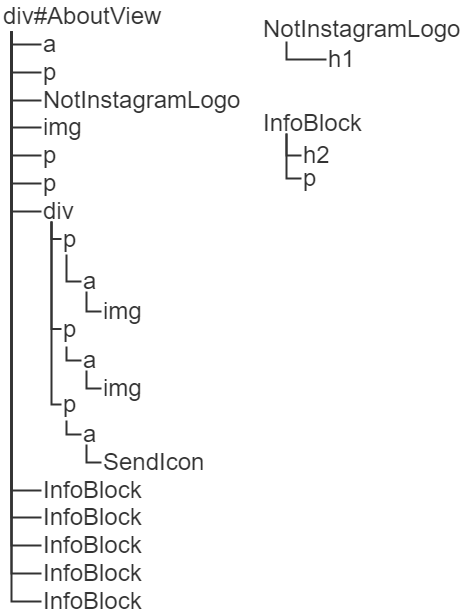
\includegraphics[width=0.4\linewidth, keepaspectratio]{diagrams/about-dom-2.png}
  \end{center}
  \caption{Graphical subdivision of the About page into components}\label{fig:graphicalAboutPage}
\end{figure}

The About page is an interesting case because, as described in section \ref{subsec:exampleapplication}, it is the only static page of the application.
Its components and \acrshort{html} children are therefore also static.
Figure \ref{fig:graphicalAboutPage} shows a graphical overview of the page's contents from a \acrshort{dom} perspective.
Because of its static nature, it is also the only page that can be fully prerendered.
Notably, the lower part of the page consists of multiple subcomponents \verb|<Infoblock>| with a title passed as a prop and a paragraph passed in a slot as a \acrshort{html} child for the component.
Functionally, its only purpose is styling and its only effect on the \acrshort{dom} is the addition of a \verb|<h2>| and a \verb|<p>| element.
The other imported subcomponents \verb|<NotInstagramLogo>| and \verb|<SendIcon>| are also wrappers for a \verb|<h1>| and a \verb|<img>| element, respectively.
Listing \ref{lst:Vue:About} demonstrates the static nature of the page view and the hard-coded addition of all text and multimedia in the template.

\vspace{1cm}
\begin{lstlisting}[caption=About page in Vue.js (as displayed in figure \ref{fig:graphicalAboutPage}), label={lst:Vue:About}, language=HTML]
<!-- AboutView.vue -->
<template>
  <div id="AboutView">
    <RouterLink id="top-backlink" class="backlink" :to="{ name: 'Feed' }"> back </RouterLink>

    <p class="cursive">This is</p>
    <NotInstagramLogo />
    <img class="transparent logo" alt="" width="40%" height="240" loading="lazy" :src="Logo" />

    <p class="cursive">created by</p>
    <p class="cursive big">Andreas Nicklaus</p>
    <div id="socials">
      <p>
        <a href="https://github.com/andreasnicklaus" target="_blank">
          <img class="transparent" width="29" height="29" loading="lazy" :src="GitHub" />
          @andreasnicklaus
        </a>
      </p>
      <p>
        <a href="https://www.linkedin.com/in/andreasnicklaus/" target="_blank">
          <img class="transparent" width="29" height="29" loading="lazy" :src="LinkedIn" />
          @andreasnicklaus
        </a>
      </p>
      <p>
        <a href="mailto:an067@hdm-stuttgart.de">
          <SendIcon/> an067@hdm-stuttgart.de
        </a>
      </p>
    </div>

    <InfoBlock title="What is this?">
      This project is part of the master thesis by ...
    </InfoBlock>
    <InfoBlock title="Placeholder 1"><!-- ... --></InfoBlock>
    <InfoBlock title="Placeholder 2"><!-- ... --></InfoBlock>
    <InfoBlock title="Placeholder 3"><!-- ... --></InfoBlock>
    <InfoBlock title="Placeholder 4"><!-- ... --></InfoBlock>
    <InfoBlock title="Placeholder 5"><!-- ... --></InfoBlock>

    <RouterLink id="bottom-backlink" class="backlink" :to="{ name: 'Feed' }"> back </RouterLink>
  </div>
</template>
\end{lstlisting}

\subsubsection{Create Page}

The Create page poses an opposite to the About page.
In contrast to a static page with non-changing content, the purpose of the Create page is to preview a new post.
Its purpose is to update after user input.
Listing \ref{lst:Vue:Create:Template} and \ref{lst:Vue:Create:Script} show the implementation of the Create page in Vue.js.
The data of the component has four dynamic parts: The options and the choice for the selection of the post image in a \verb|<select>| element, the caption of the new post and the media \acrshort{url} for the \verb|<input>| element.
The last data point for the component is the user handle, which is static for the preview in this example application.
The computed property \verb|mediaSource| (see listing \ref{lst:Vue:Create:Script}, line \ref{line:computedMediaSource:createPage}) represents the logical choice between the media selection and source \acrshort{url} for the multimedia file in the previewed post.
This template contains a static \verb|<header>|, the \verb|<form>| with dynamic attributes and a Post component.
This subcomponent has to be dynamic and reactive to its props as they are changing throughout the process of post creation.

\vspace{1cm}
\begin{lstlisting}[caption=Create page in Vue.js (Template), label={lst:Vue:Create:Template}, language=HTML]
<!-- CreateView.vue -->
<template>
  <header>
    <RouterLink :to="{ name: 'Feed' }"> <NotInstagramLogo/> </RouterLink>
    <RouterLink :to="{ name: 'Feed' }"> <XIcon/> </RouterLink>
  </header>

  <form id="newPostForm" action="" method="post">
    <input type="url" name="mediaUrl" id="mediaUrl" placeholder="Insert your media URL here..." v-model="mediaUrl" />
    <p>or</p>
    <select name="preloaded-image" id="preloaded-image" v-model="mediaChoice">
      <option value="">Choose one of our media files here...</option>
      <option v-for="media in preloadedMedia" :key="media" :value="media">
        <span>{{ media }}</span>
      </option>
    </select>
    <textarea name="caption" id="caption" cols="30" rows="3" placeholder="Type your caption here" v-model="caption"/>
    <button type="submit" :disabled="!(caption && mediaSource)"> Post it! </button>
  </form>

  <hr />

  <Post :userhandle="userhandle" :caption="caption" :likeCount="0" :mediaSource="mediaSource" :hideActionIcons="true" />
</template>
\end{lstlisting}
\hrule
\begin{lstlisting}[caption=Create page in Vue.js (Script), label={lst:Vue:Create:Script}, language=JavaScript, firstnumber=25, escapechar=°]
// CreateView.vue
export default {
  name: "CreateView",
  data() {
    return {
      preloadedMedia: [
        "canyon.mp4", "abstract-circles.webp", ...
      ],
      userhandle: "@you",
      caption: "",
      mediaUrl: "",
      mediaChoice: "",
    };
  },
  computed: {
    mediaSource() { °\label{line:computedMediaSource:createPage}°
      return this.mediaUrl || this.mediaChoice;
    },
  },
};
\end{lstlisting}
\vspace{1cm}

Listings \ref{lst:Vue:Post:Template} and \ref{lst:Vue:Post:Script} show the implementation of the Post component in Vue.js.
It requires five props for the five data points of a post (see figure \ref{fig:classes}) and two additional props for the control over the design and loading behaviour of the post's image or video.
Additionally, the \verb|mounted| method loads the user data through the \verb|ProfileService| (see listing \ref{lst:Vue:Post:Script}, line \ref{line:postMounted}).
The template of the component uses MediaComponent twice, once for the profile picture and once for the post image or video.
The attributes for the profile picture are mainly static because the user data is not edited through the create form.
The attributes of the post multimedia are dynamic and editable except the class, width and height.
Additionally, the projection of the post's caption onto the \acrshort{dom} is dynamic.
Every time the caption changes, the string is split by whitespaces and each word is projected onto a \verb|<span>| element, so it can be styled as a hashtag if applicable.
Afterwards, the list of \verb|<span>| elements is joined using whitespaces.
The purpose of this projection method for the caption is only the styling of hashtags.

\vspace{1cm}
\begin{lstlisting}[caption=Post in Vue.js (Template), label={lst:Vue:Post:Template}, language=HTML]
<!-- Post.vue -->
<template>
  <div class="post">
    <RouterLink v-if="user" :to="{ name: 'Profile', params: { handle: userhandle } }" class="postUserInfo" >
      <MediaComponent class="profileImage" :src="user?.profileImageSource" alt="" width="44" height="44" />
      <span class="username">{{ user?.username }}</span>
    </RouterLink>
    <MediaComponent class="postMedia" :src="mediaSource" :alt="caption" width="100%" height="100%" :eagerLoading="eagerLoading" />
    <div class="actionIconRow" v-if="!hideActionIcons">
      <div class="leftActionIcons">
        <HeartIcon />
        <CommentIcon />
        <SendIcon />
      </div>
      <BookmarkIcon />
    </div>
    <p class="likeCount">{{ likeCount }} likes</p>
    <p class="caption">
      <span v-for="(word, i) in caption.split(' ')" :key="i" :style="word.startsWith('#') ? 'color: #0091E2' : ''">
        {{ word }}{{ " " }}
      </span>
    </p>
    <p class="creationTime">{{ creationTimeToString }}</p>
  </div>
</template>
\end{lstlisting}
\hrule
\begin{lstlisting}[caption=Post in Vue.js (Script), label={lst:Vue:Post:Script}, language=JavaScript, firstnumber=26, escapechar=°]
// Post.vue
import ProfileService from "@/services/ProfileService";

export default {
  name: "Post",
  props: {
    userhandle: String,
    caption: String,
    mediaSource: String,
    likeCount: Number,
    createdAt: Date,
    hideActionIcons: Boolean,
    eagerLoading: { type: Boolean, default: false },
  },
  data() {
    return { user: null };
  },
  mounted() {°\label{line:postMounted}°
    ProfileService.getByHandle(this.userhandle).then((user) => (this.user = user));
  },
  computed: {
    creationTimeToString() {
      // ...
    },
  },
};
\end{lstlisting}
\vspace{1cm}

Because the creation of such a dynamic component is an intended use case for Angular, Next.js, Nuxt, React, Svelte and Vue.js, their implementation is not unusual.
Astro poses as an opposite to this.
Because dynamic or reactive components are not implementable natively as Astro components, another framework has to be used in Astro Islands.
For this reason, other components had to be invented in addition to the components as described in figure \ref{fig:uml}.
\verb|CreateForm| encapsulates the dynamic parts of the Create page.
It is a React component with the form and post preview.
Because Astro components cannot be used in Islands, every subcomponent used here had to be implemented with React as a duplicate to an Astro component.

Listings \ref{lst:Astro:Create:Script}, \ref{lst:Astro:Create:HTML} and \ref{lst:Astro:Createform} show the implementation of this unique design in Astro.
The Create component imports and inserts the React component \verb|CreateForm| into \acrshort{html} snippets for the page and marks it as a \acrshort{csr} component with \verb|client:load| (see listing \ref{lst:Astro:Create:HTML}, line \ref{line:clientLoad}).
From this component inwards, all \acrshort{html} is generated on the client and purely as a React application.
The CreateForm itself contains the form and Post subcomponent.
Because of this structure, the components Post, MediaComponent, BookmarkIcon, CommentIcon, HeartIcon and SendIcon had to be implemented as Astro components and as React components.
Figure \ref{fig:astroUml} shows this updated component structure with Astro Islands.

\vspace{1cm}
\begin{lstlisting}[caption=Create page in Astro (Frontmatter), label={lst:Astro:Create:Script}, language=JavaScript]
// create.astro 
export const prerender = false;
import HtmlLayout from "../Layouts/HtmlLayout.astro";
  
import NotInstagramLogo from "../components/NotInstagramLogo.astro";
import XIcon from "../components/icons/XIcon.astro";
import CreateForm from "../components/CreateForm.jsx";
import React from "react";

const userhandle = "@you";
\end{lstlisting}
\hrule
\begin{lstlisting}[caption=Create page in Astro (HTML), label={lst:Astro:Create:HTML}, language=HTML, firstnumber=11, escapechar=°]
<!-- create.astro -->
<HtmlLayout>
  <header>
    <a href="/"> <NotInstagramLogo /> </a>
    <a href="/"> <XIcon /> </a>
  </header>
  <React.StrictMode>
    <CreateForm userhandle={userhandle} client:load />°\label{line:clientLoad}°
  </React.StrictMode>
</HtmlLayout>
\end{lstlisting}
\hrule
\begin{lstlisting}[caption=Create form in Astro, label={lst:Astro:Createform}, language=JavaScript]
// CreateForm.jsx
import { useState } from "react";
import styles from "./CreatePost.module.css";
import Post from "./Post";

const preloadedMedia = [
  "canyon.mp4", "abstract-circles.webp", // ...
];

const CreateForm = ({ userhandle }) => {
  const [caption, setCaption] = useState("");
  const [mediaUrl, setmediaUrl] = useState("");
  const [mediaChoice, setmediaChoice] = useState("");

  function mediaSource() { return mediaUrl || mediaChoice; }

  return (
    <>
      <form id={styles.newPostForm} action="" method="post">
        <input type="url" name="mediaUrl" id={styles.mediaUrl} placeholder="Insert your media URL here..." value={mediaUrl} onChange={(event) => setmediaUrl(event.target.value)} />

        <p>or</p>

        <select name="preloaded-image" id={"preloaded-image"} value={mediaChoice} onChange={(event) => setmediaChoice(event.target.value)}>
          <option value="">Choose one of our media files here...</option>
          {preloadedMedia.map((media) => (
            <option key={media} value={media}>{media}</option>
          ))}
        </select>
        <textarea name="caption" id={styles.caption} cols="30" rows="3" placeholder="Type your caption here" value={caption} onChange={(event) => setCaption(event.target.value)}/>
        <button type="submit" disabled={!(caption && mediaSource())}> Post it! </button>
      </form>
      <Post userhandle={userhandle} caption={caption} likeCount={0} mediaSource={mediaSource()} hideActionIcons={true} />
    </>
  );
};

export default CreateForm;
\end{lstlisting}
\vspace{1cm}

\begin{figure}[h!]
  \begin{center}
    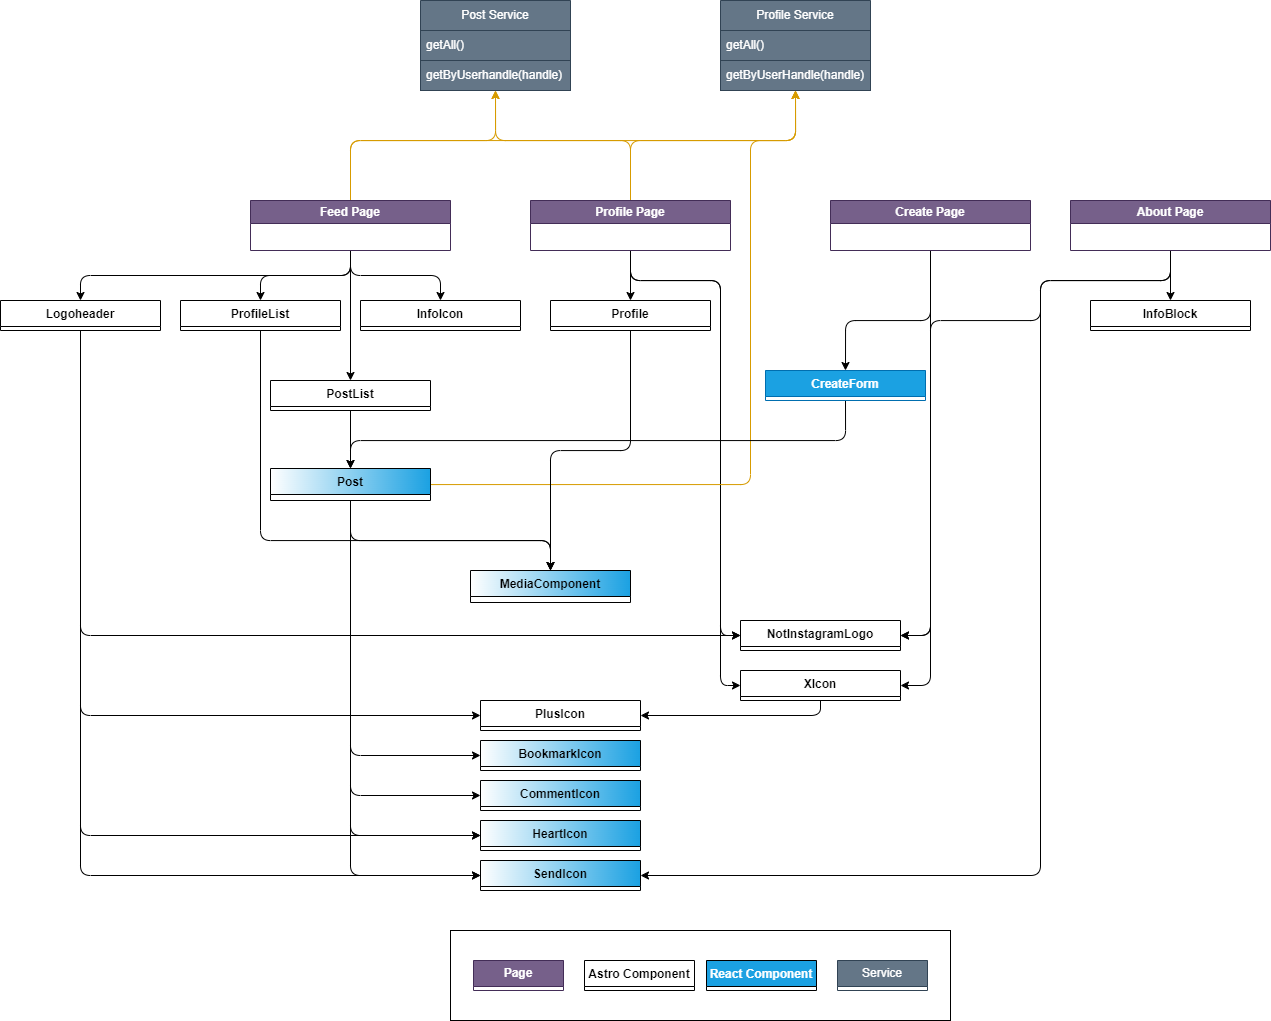
\includegraphics[width=\linewidth]{diagrams/uml-astro.png}
  \end{center}
  \caption{Adapted component structure for Astro Islands}\label{fig:astroUml}
\end{figure}

\subsubsection{MediaComponent}

MediaComponent is a presenter component for multimedia content, namely an image or a video.
It is used within the ProfileList, Profile and Post components (see figure \ref{fig:uml}).
As described in section \ref{subsec:exampleapplication}, the main use of this component for a developer is to centralize the optimization of multimedia files and to ensure its correct size and style.
As such, it is a catch-all component for many kinds of multimedia sources. Listings \ref{lst:Vue:MediaComponent:Template} and \ref{lst:Vue:MediaComponent:Script} show parts of its implementation in Vue.js.

\vspace{1cm}
\begin{lstlisting}[caption=MediaComponent in Vue.js (Template), label={lst:Vue:MediaComponent:Template}, language=HTML]
<!-- MediaComponent.vue -->
<template>
  <img ref="image" class="postMedia" v-if="mediaSource.endsWith('webp')" :alt="alt" :width="width" :height="height" :loading="eagerLoading ? 'eager' : 'lazy'" :src="mediaSource" />
  <video ref="video" class="postMedia" v-else-if="mediaSource.endsWith('mp4')" :width="width" :preload="eagerLoading ? 'auto' : 'metadata'" controls controlslist="nodownload,nofullscreen,noremoteplayback" disablepictureinpicture loop muted >
    <source :src="mediaSource" type="video/mp4" />
  </video>
  <div v-else class="mediaError" ref="mediaError">
    <p>Nothing to see yet...<br />Choose an image to continue!</p>
  </div>
</template>
\end{lstlisting}
\hrule
\begin{lstlisting}[caption=MediaComponent in Vue.js (Script), label={lst:Vue:MediaComponent:Script}, language=JavaScript, firstnumber=13, escapechar=°]
// MediaComponent.vue
import { playPauseVideo } from "@/utils/autoplay.js";

export default {
  name: "MediaComponent",
  props: {°\label{line:mediaComponentProps}°
    src: { type: String },
    alt: { type: String,  default: "" },
    width: String,
    height: String,
    eagerLoading: { type: Boolean, default: false },
  },
  computed: {
    mediaSource() {°\label{line:computedMediaSource}°
      if (
        this.src == null ||
        this.src == undefined ||
        this.src.startsWith("http")
      )
        return this.src;
      return new URL(`/src/assets/stock-footage/${this.src}`, import.meta.url).href;
    },
  },
  mounted() {
    const video = this.$refs.video;
    if (video) playPauseVideo(video);
  },
};
\end{lstlisting}
\vspace{1cm}

First, the component takes five props that can be passed to it as \acrshort{html} attributes (see listing \ref{lst:Vue:MediaComponent:Script}, line \ref{line:mediaComponentProps} ff.).
The \verb|src| string contains either the file name or \acrshort{url} to the file.
The \verb|alt| prop is the alternative text for an image to simple pass to the \verb|alt| attribute of the \verb|<img>| tag, as well as the width and height of the image or video.
These props are primarily needed for optimization of layout shifts and to optionally tell the browser which image variant is needed from a source set on the page.
Lastly, the \verb|eagerLoading| prop is a boolean indicator for whether the file needs to be loaded first (images) or preloaded fully (videos).

Second, the computed property \verb|mediaSource| returns the correct link to either the image or video source based on the start of the \verb|src| prop.
This allows the component to identify faulty or external source \acrshort{url}s and only import needed local multimedia files.
This implementation design is unique to Vue.js and Nuxt.
Looking at the implementation in React and Next.js, the same effect is achieved through the \verb|useState| and \verb|useEffect| hooks.
The \verb|ngOnChanges| hook is used in Angular.
In Svelte, the \verb|mediaSource| is defined with a leading \verb|$:|, making it reactive. Because of its non-dynamic nature the native Astro component defines \verb|mediaSource| statically server-side.
On the other hand, the dynamic component uses the same implementation as the React application.

Third, every framework uses conditional rendering to project either an image, a video or an error message onto the \acrshort{dom}.
Additionally, the Svelte component checks another condition: external and internal images.
For image source strings starting with \enquote{http}, an \acrshort{html}-native \verb|<img>| element is used, whereas the Svelte-native \verb|<enhanced:img>| tag is used for all other images.
The remaining frameworks use either one or the other method to insert images.
Vue.js, React and Angular do not support enhanced image elements.
These frameworks only include images using the \verb|<img>| tag.
In contrast, Astro, Next.js, Nuxt and Svelte do have components that improve the performance of image elements.
Astro natively supports an \verb|<Image>| component that outputs an \verb|<img>| tag with optimized attributes.
Next.js comes with another \verb|<Image>| component that optimizes images with a predefined width and height and Nuxt has a \verb|<NuxtImg>| component to optimize images and define presets for its images.
Svelte is the only one of this group that does not support full \acrshort{url}s to be passed to its enhanced image component.

Fourth, the attributes of the \verb|<img>| elements are designed to optimize their load performance, size and image quality.
While no way to optimize the size and quality of the source of simple \verb|<img>| elements is apparent, the load performance is adapted to the usage of a \verb|<MediaComponent>|.
The first Post of a PostList is always eager-loaded, whereas all other images are lazy-loaded.
The size of the bounding box of the image is also defined in order to prevent layout shifts during or after the loading of the image.
Enhanced image components are configured to ideally optimize the size and quality of the requested image, as well as to insert blurry placeholder images if possible.

The \verb|<video>| elements are designed to optimize the load behaviour of the browser and to change the default presentation and styling.
Each video has a defined width and height, playback behaviour and controls.
In order to come as close to the application's model, Instagram, videos should autoplay, but be muted by default.
Each single behaviour is a single attribute to set, but autoplaying every video requires every video to be loaded on page load.
This network load bears a performance decrease.
For this reason, only the metadata is preloaded unless it is the first post in the PostList.
To ensure the wanted autoplay feature, each \verb|<video>| element is referenced using the framework and custom code ensures that videos play when they are in the viewport and pause when they are outside of it.
This is achieved using an \verb|IntersectionObserver| \citep{IntersectionObserver}.

\subsection{Configuration of testing tools}\label{subsec:tests}
% How are tests configured and implemented?
% What is measured, stored and evaluated?
% 
% - Test categories
%   - Page Load
%   - Dynamic Component Load Times
%   - State Change Times
% - Playwright test configuration
%   - Tests
%   - Attachments
%   - Screenshots
% - Browser Choices: Reasoning and test implementation

As described above, the implemention of tests and test configuration were the last step in the process of project creation.
As such, tests were either left \enquote{as is} or not configured until the application could be considered \enquote{done}.
The test suite for this project can be split into two halves: Lighthouse \acrshort{cli} automation and Playwright tests (see section \ref{subsec:testingtools}).
Lighthouse is used to mostly cover aggregate metrics, while Playwright is used to export navigation and \acrshort{html} event times.

\subsubsection{Lighthouse}

To this end, a script was written to automate the execution of Lighthouse tests and to store Lighthouse reports in a comprehensive way.
Listing \ref{lst:lighthouse-script} shows parts of the implementation of the testing script.
It reads project configurations from an external configuration file and iterates over them, executing the tests for every framework multiple times.
Listing \ref{lst:lighthouse-config} contains an excerpt of the configuration file.
Every project is built and hosted, if either a host command, e.g. using \verb|npm run <script>|, or a serve command using \verb|serve| is defined in the configuration file.
While the application is hosted, a headless Google Chrome browser window is launched and multiple lighthouse tests are preformed.
The report is generated using the \acrshort{url} as it is specified in the configuration and with static options.
These options define among other things that an \acrshort{html} report is to be generated, only performance metrics are to be collected and the \acrshort{http} status code is to be ignored.
The last option is necessary because web servers started using \verb|serve| return a 404 status code for files that do not exist in the hosted directory.
For applications that rely on \verb|index.html| to be returned if a requested resource is not available, this behaviour is not desired.
For example, requesting the defined path \verb|/about| results in a 404 code with the \verb|index.html| file as the response body.
Withouth the option \verb|ignoreStatusCode: true|, the Lighthouse test would fail as the page is considered to be unavailable.

\vspace{1cm}
\begin{lstlisting}[caption={Automation script for Lighthouse tests}, language=JavaScript, label={lst:lighthouse-script}]
// testing-script/index.js
// ...

function build(projectConfig) {
  return new Promise((resolve, reject) => {

    if (projectConfig.buildCommand) {
      logger.info("Starting build...")
      exec(`${projectConfig.buildCommand}`, /* ... */)
    }
    else {
      logger.info("Skipping build because buildCommand was not specified")
      resolve()
    }
  })

}

// ...

for (let projectConfig of config.projects) {
  //  ...
  // BUILD PHASE
  await build(projectConfig)

  // STARTING HOST PROCESS
  // ...

  // START LIGHTHOUSE TEST
  logger.info("Starting lighthouse tests...")
  const url = projectConfig.url
  const chrome = await chromeLauncher.launch( { chromeFlags: ['--headless'] } );
  const options = { logLevel: 'warn', output: 'html', onlyCategories: ['performance'], port: chrome.port, ignoreStatusCode: true };

  for (const route of (projectConfig.paths || ["/"])) {
    // ...

    for (let i = 0; i < config.runsPerProject; i++) {

      const runnerResult = await lighthouse(url + route, options);

      const { report: reportHtml, artifacts, lhr } = runnerResult;
      const { timing, fetchTime, categories, ...rest } = lhr

      fs.mkdirSync(`${projectConfig.reportDirectory}${route == "/" ? "/index" : route}`, { recursive: true }, (err) => {
        if (err) throw err;
      });
      fs.writeFileSync(`${projectConfig.reportDirectory}${route == "/" ? "/index" : route}/lighthouse-report-${new URL(url).hostname}-${dateToUriSafeString(new Date())}.html`, reportHtml);
      fs.writeFileSync(`${projectConfig.reportDirectory}${route == "/" ? "/index" : route}/lighthouse-report-${new URL(url).hostname}-${dateToUriSafeString(new Date())}.json`, JSON.stringify({ artifacts, lhr }, null, 2));

      // ...
    }

    // ...
  }

  await chrome.kill();
  if (serverCommand) await stopServer(hostProcess, projectConfig)
}

logger.info("ALL DONE")
\end{lstlisting}
\hrule
\begin{lstlisting}[caption={Test configuration for Lighthouse tests}, language=JavaScript, label={lst:lighthouse-config}]
// testing-script/config.js
export default {
  runsPerProject: 20,
  preferredServeCommand: "serve",
  projects: [
    // ...
    {
      name: "Svelte on Vercel",
      reportDirectory: "./reports/ig-clone-svelte/vercel",
      url: "https://ig-clone-svelte.vercel.app",
      paths: ["/", "/about", "/create", "/user/@PeterPoster"]
    },
    // ...
    {
      name: "Svelte",
      projectPath: "../ig-clone/ig-clone-svelte",
      buildCommand: "npm run build",
      serveCommand: "npm run preview",
      reportDirectory: "./reports/ig-clone-svelte/localhost",
      url: "http://localhost:4173",
      paths: ["/", "/about", "/create", "/user/@PeterPoster"]
    },
    // ...
  ]
}
\end{lstlisting}
\vspace{1cm}

Once the test results are available, the relevant metrics are collected, stored in a \acrshort{json} file and the \acrshort{html} report is stored as a means to debugging.
After the tests are finished and results are stored, the Google Chrome window is killed and the webserver is stopped.

In order to evaluate and summarize the collection of tests performed using the automation script, another script was written so that test summaries are created.
This report reader iterates over the list of \acrshort{json} files and calculates the average per metric, route and project configuration from the configuration file.
It makes it easier to compare the test results and interpret the performance of the frameworks (see chapter \ref{sec:evaluation}).

\subsubsection{Playwright}

Similar to the test method for Lighthouse, Playwright tests can be triggered using a script to unify the output files.
Listing \ref{lst:playwright-trigger} shows the implementation of this trigger script.
Project directories are defined and the test command is executed in the directory with the configured environment variables.
Playwright is told to not open a report even if a test fails through \verb|PW_TEST_HTML_REPORT_OPEN|.

\vspace{1cm}
\begin{lstlisting}[caption={Trigger script for Playwright tests}, label={lst:playwright-trigger}, language=JavaScript]
// playwright-trigger.mjs
import { spawn } from 'child_process'

const projects = [
  // ...
  {
    name: "IG Clone Svelte",
    cwd: "ig-clone-svelte"
  },
]

const testArguments = [/* "/.*change\.spec\.js/" */]
function generateUriSafeTimestamp() {/* ... */ }
// ...

for (const project of projects) {
  // ...
  const now = new Date()
  const reportDirectory = `playwright-report-${generateUriSafeTimestamp()}`

  await new Promise(resolve => {
    const testProcess = spawn("npm", ["run", "test:e2e", ...testArguments], {
      cwd: project.cwd,
      shell: true,
      env: {
        ...process.env,
        PW_TEST_HTML_REPORT_OPEN: 'never'
      }
    })
    // ...
  })
}
\end{lstlisting}
\hrule
\begin{lstlisting}[caption={Playwright configuration for Vue.js}, label={lst:playwright-config}, language=JavaScript]
// ig-clone-vue/playwright.config.js
import process from 'node:process'
import { defineConfig, devices } from '@playwright/test'

export default defineConfig({
  testDir: './tests',
  timeout: 60 * 1000,
  expect: { timeout: 5000 },
  retries: 2,
  workers: 1,
  reporter: [['html'], ['json', { outputFile: 'playwright-report/test-results.json' }]],
  use: {
    baseURL: 'http://localhost:3000',
    trace: 'on',
    headless: true
  },

  projects: [
    { name: 'Chromium', use: {...devices['Desktop Chrome']} },
    { name: 'Firefox', use: {...devices['Desktop Firefox']} },
    { name: 'Desktop Safari', use: {...devices['Desktop Safari']} },
    { name: 'Mobile Chrome', use: {...devices['Pixel 5']} },
    { name: 'Mobile Safari', use: {...devices['iPhone 12']} },
    { name: 'Microsoft Edge', use: {channel: 'msedge'} },
    { name: 'Google Chrome', use: {channel: 'chrome'} },
  ],

  webServer: {
    command: 'vite build && serve -sd dist',
    port: 3000,
    reuseExistingServer: true
  }
})

\end{lstlisting}
\vspace{1cm}

The tests and test configuration are similar for all frameworks.
Listing \ref{lst:playwright-config} shows how the test suite is configured.
Timeouts are defined for all tests so that even slowly loading pages are tested properly and retries are specified to repeat failing tests twice.
The reason for this specification is that fluctuating timings close to the limit of failure should be tested multiple times to ensure that the test is supposed to fail.
Unfortunately, repetitions cannot be configured for the opposite case in which the test passes because of fluctuations, but is supposed to fail on average.
All test executions and repetitions are configured to run in sequence to minimize the influence of the availability of resources on the testing machine.
This is especially important because Playwright both opens the application in a browser and runs a webserver for local tests.
It is set to start a webserver, wait for its availability and then open the application under the specified \verb|baseURL|.
The webserver command, port and \verb|baseURL| are different for every framework.
The test configuration also specifies a list of browsers to test the application in.
For this study, seven browsers were chosen based on the most used browsers \citep{browserUsage} and their mobile versions.
The browsers are Chromium, Google Chrome, Mobile Chrome, Safari, Mobile Safari, Microsoft Edge and Firefox.

The tests written for this application are threefold as they reflect the separation of performance metrics (see section \ref{subsec:performancemetrics}).
Listings \ref{lst:page-load-spec}, \ref{lst:dynamic-performance-spec} and \ref{lst:state-change-spec} show the test files.

First, page load times are measured using \verb|page-load.spec.js| (see listing \ref{lst:page-load-spec}).
Every defined route is opened in a browser window, the navigation timings are extracted through a \verb|page.evaluate(<evalFunction>)| method and the timings are attached and annotated so that they can be read after the test execution.
The test for every page is that the timings \verb|loadEventEnd| and \verb|domComplete| are faster than a time budget.
The paths and time budget per page configed in \verb|pages.js| (see listing \ref{lst:pages-config}).
To ensure a fast performance, the time budgets are defined to be under two seconds for all pages.
Because no network requests are made in the design of the application on the About page, the time budget was lowered to 1.5 seconds here.

\vspace{1cm}
\begin{lstlisting}[caption={Test file for page load times}, label={lst:page-load-spec}, language=JavaScript]
// page-load.spec.js
import { test, expect } from '@playwright/test';
import routes from "./pages.js"

test.describe("Load Time", () => {
  for (const route of routes) {
    test(`${route.name} loads within the page load budget`, { tag: [`@${route.name}`, '@pageLoad'] }, async ({ page }, TestInfo) => {

      await page.goto(route.path)
      await page.waitForLoadState()

      const timing = await page.evaluate(() => performance.getEntriesByType('navigation'));
      TestInfo.attach("timing.json", { body: JSON.stringify(timing, null, 2), contentType: "application/json" })

      const [{ responseStart, responseEnd, domContentLoadedEventEnd, domComplete, loadEventEnd }] = timing;

      test.info().annotations.push({ type: 'Page Load Budget', description: `The time budget for this page was ${route.pageLoadBudgetMs}ms` });
      // ...

      expect.soft(domComplete, `domComplete event should happen within ${route.pageLoadBudgetMs} ms`).toBeLessThanOrEqual(route.pageLoadBudgetMs)
      expect.soft(loadEventEnd, `loadEventEnd event should happen within ${route.pageLoadBudgetMs} ms`).toBeLessThanOrEqual(route.pageLoadBudgetMs)
    })
  }
})
\end{lstlisting}
\hrule
\begin{lstlisting}[caption={Test pages configuration}, label={lst:pages-config}, language=JavaScript]
// pages.js
const routes = [
  { name: "Feed page", path: "/", pageLoadBudgetMs: 2000 },
  { name: "About page", path: "/about", pageLoadBudgetMs: 1500 },
  { name: "Create page", path: "/create", pageLoadBudgetMs: 2000 },
  { name: "Profile page", path: "/user/@PeterPoster", pageLoadBudgetMs: 2000 },
]

export default routes;
\end{lstlisting}
\vspace{1cm}

Second, \verb|dynamic-performance.spec.js| describes how component load times are measured.
The same routes are opened after an initialization script is injected into the browser window.
Listings \ref{lst:dynamic-performance-spec} and \ref{lst:performance-recorder} show parts of the test definition and the injected script.
The latter waits for a specific element to appear in the \acrshort{dom} that does not appear in the \acrshort{html} skeleton, if it exists.
The element in question has a predetermined \verb|id|.
For Angular, Astro, Next.js, Svelte and Vue.js it is \enquote{app}, for Nuxt it is \enquote{\_\_nuxt} and for React it is \enquote{root}.
Afterwards, it initializes a \verb|MutationObserver| on that element.
Each observation is stored with an xpath, id and the last mutation time.
The mutation time is overwritten every time so that only the latest update is recorded and the list of times is published as a member of the window object.
Recorded mutations are added or removed children, addition or removal of the element itself and a changed attribute.
Because the time of mutation is only measured as the time difference to the addition of the application-specific root element, the recorded times are an estimation of the execution time between framework initialization and the latest \acrshort{dom} mutation.

The test script waits for ten seconds after the injection of the recording script and then evaluates the recorded timings.
The update times are also attached to the test as a \acrshort{json} file so that they can be traced after the test context no longer exists.
In order for the test to pass for the page the latest \acrshort{dom} mutation needs to happen within the page's load time budget.
In order to trace the failing components more easily, screenshots are taken of each slow \acrshort{html} element.
Additionally, a screenshot of the whole page is taken in which slow elements are colored. Every screenshot is then attached to the test.
This method ensures that slow components can be identified visually even if the xpath and the id of the element changes between component lifecycles or application builds.

\vspace{1cm}
\begin{lstlisting}[caption={Test file for component load times}, label={lst:dynamic-performance-spec}, language=JavaScript, escapechar=°]
// dynamic-performance.spec.js
import { test, expect } from '@playwright/test';
import routes from "./pages"

test.describe("Dynamic load time", () => {
  for (const route of routes) {
    test(`Dynamic components on ${route.name} load within the load budget`, { tag: [`@${route.name}`, '@componentLoad'] }, async ({ page }, TestInfo) => {
      // Inject performance measurement script into the page
      await page.addInitScript({ path: './tests/performance.js' })

      // Go to the measured page
      await page.goto(route.path)
      await page.waitForLoadState('domcontentloaded')

      // Start evaluation
      const latestUpdateComponents = await new Promise(resolve => setTimeout(resolve, 10_000)).then(() => {°\label{line:dynamic-performance-spec:maxTime}°
        // Return the sorted load times
        return page.evaluate(() => {
          if (!window.dynamic_component_performance) return null
          // Sort the components by their latest dom update time
          const sortedEntries = Object.entries(window.dynamic_component_performance)
            .map(([key, value]) => { return { id: key, ...value } })
            .sort((a, b) => a.lastUpdated - b.lastUpdated)
          return sortedEntries
        })
      })

      // Attach the measurements in JSON format
      TestInfo.attach("update-times.json", { body: JSON.stringify(latestUpdateComponents, null, 2), contentType: "application/json" })

      latestUpdateComponents.forEach(comp => {
        const latestUpdateTime = comp.lastUpdated

        // Assert the latest update occurs in time
        return expect.soft(latestUpdateTime, `Component with identifier ${comp.id} should load within ${route.pageLoadBudgetMs} ms`).toBeLessThan(route.pageLoadBudgetMs)
      })

      // Create screenshots of slow components
      const componentScreenshots = await Promise.all(
        latestUpdateComponents.map((el) => {
          if (el.lastUpdated > route.pageLoadBudgetMs) {
            return page.locator(el.id).screenshot().then(screenshot => [el, screenshot])
          }
        }).filter(i => i)
      )

      // Capture a screenshot of the whole page with highlighted slow components
      if (latestUpdateComponents.some(comp => comp.lastUpdated > route.pageLoadBudgetMs)){
        // ...
      }

      // Attach the screenshots of the slow components to the test
      await Promise.all(componentScreenshots.map(([el, screenshot]) => {
          return TestInfo.attach( `${el.id}-${el.lastUpdated}ms.png`, {body: screenshot, contentType: 'image/png'})
        })
      )
    })
  }
})
\end{lstlisting}
\hrule
\begin{lstlisting}[caption={Injected mutation recorder script}, label={lst:performance-recorder}, language=JavaScript, escapechar=°]
// performance.js
let loadTimes = {}
let startTime = Date.now()

function observe(targetNode) {
  // Options for the observer (which mutations to observe)
  const config = { attributes: true, childList: true, subtree: true };

  // Callback function to execute when mutations are observed
  const callback = (mutationList, observer) => {
    for (const mutation of mutationList) {

      if (mutation.type === "childList") {
        const targetId = getId(mutation.target)

        const skipAttribute =
          mutation.target.attributes.skipperformance?.value ||
          mutation.target.attributes.skipPerformance?.value

        if (!(skipAttribute == true || skipAttribute == 'true')) {

          if (mutation.addedNodes.length > 0) {
            let addedElements = Array.from(mutation.addedNodes).map(el => el.nodeName !== "#comment" && el.nodeName !== "#text" ? getXPath(el) : el)
            if (addedElements.length === 1) addedElements = addedElements[0]

            if (Array.from(mutation.addedNodes)) {
              loadTimes[targetId] = { ...loadTimes[targetId], lastUpdated: Date.now() - startTime, xpath: loadTimes[targetId]?.xpath || getXPath(mutation.target) }

              Array.from(mutation.addedNodes).forEach(node => {
                try {
                  const nodeId = getId(node)
                  loadTimes[nodeId] = { ...loadTimes[nodeId], lastUpdated: Date.now() - startTime, xpath: loadTimes[nodeId]?.xpath || getXPath(node)}
                } catch (e) {
                  console.warn(e)
                }
              })
            }
          }

          else if (mutation.removedNodes.length > 0) {
            // same as above ...
          }

        }

      } else if (mutation.type === "attributes") {
        const targetId = getId(mutation.target)

        const skipAttribute =
          mutation.target.attributes.skipperformance?.value ||
          mutation.target.attributes.skipPerformance?.value

        if (!(skipAttribute == true || skipAttribute == 'true')) {
          loadTimes[targetId] = { ...loadTimes[targetId], lastUpdated: Date.now() - startTime, xpath: loadTimes[targetId]?.xpath || getXPath(mutation.target) }
        }

      }
    }

    window.dynamic_component_performance = loadTimes
  };

  // Create an observer instance linked to the callback function
  const observer = new MutationObserver(callback);

  // Start observing the target node for configured mutations
  observer.observe(targetNode, config);
}

function getId(element) {/* ... */}
function getXPath(element) {/* ... */}

function reset() {
  loadTimes = {}
  startTime = Date.now()
}

let interval;

function initObservation() {
  // The id of the targetNode has to be adapted to the framework or application
  const targetNode = document.getElementById("app")
  if (targetNode) {
    observe(targetNode)
    if (interval) clearInterval(interval)
  }
}

interval = setInterval(initObservation, 100) °\label{line:mutationInterval}°

// initialize window.dynamic_component_performance
window.dynamic_component_performance = loadTimes
\end{lstlisting}
\vspace{1cm}

Third, tests in \verb|state-change.spec.js| specify measurements for component update times (see listing \ref{lst:state-change-spec}).
In this test specification, two other time budgets are defined.
The first update to the \acrshort{dom} and the slowest update to the \acrshort{dom} are tested.
The idea behind these time budgets is that users may perceive the \enquote{reaction time} as the time frame in which their action had any effect or as the time frame in which the effects of their actions finish.
To this end, user actions are defined in combination with a route to perform these actions on.
For this work, four actions are defined on the Create page: The changing of the caption, the selection of an image, the insertion of a media source \acrshort{url} and the creation of a new post, which is a combination of caption change and media selection.

In order to evaluate the reaction speed to those user actions, the same mutation recording script is injected as for component load times.
The page is then opened and the recorded mutation timings are reset. Afterwards, the user action is performed and the new mutation times are extracted, attached to the test and evaluated.
The requirements for the tests to pass are that the earliest mutation timing is within 100 ms of the user input and the latest mutation timing is within 500 ms of the user input.
Again, screenshots are taken of all \acrshort{html} elements that were recorded as mutated and do not pass the tests.
These screenshots are also attached to the test in order to debug applications that do no pass the tests.

\vspace{1cm}
\begin{lstlisting}[caption={Test file for component update times}, label={lst:state-change-spec}, language=JavaScript, escapechar=°]
// state-change.spec.js
import { test, expect } from '@playwright/test';

const minReactionTime = 100;
const maxUpdateTime = 500;

const actions = [
  {
    route: '/create',
    inputActions: [
      {
        name: 'Caption Change',
        action: async (page) => {
          const captionInputField = page.getByPlaceholder('Type your caption here')
          return captionInputField.fill('Lorem ipsum ...')
        }
      },
      {
        name: 'Media Selection',
        action: async (page) => {
          const mediaSelector = page.locator('#preloaded-image')
          return mediaSelector.selectOption('moon.webp')
        }
      },
      {
        name: 'Media Source Insert',
        action: async (page) => {
          const captionInputField = page.getByPlaceholder('Insert your media URL here...')
          return captionInputField.fill(`${new URL(await page.url()).origin}/abstract-circles.webp`)
        }
      },
      {
        name: 'Post Creation',
        action: async (page) => {
          const mediaSelector = page.locator('#preloaded-image')
          const captionInputField = page.getByPlaceholder('Type your caption here')
          await mediaSelector.selectOption('moon.webp')
          return captionInputField.fill('Lorem ipsum ...')
        }
      }
    ]
  }
]

for (const actionGroup of actions) {
  for (const inputAction of actionGroup.inputActions) {

    test.describe(`State Change DOM Update: ${inputAction.name}`, { tag: [`@${inputAction.name.replace(/\s/g, '')}`, '@stateChange'] }, () => {
      let page;
      let domUpdates = null;

      test.beforeAll(async ({ browser }) => {
        page = await browser.newPage();
        await page.addInitScript({path: './tests/performance.js'})

        await page.goto(actionGroup.route)
        await page.waitForLoadState('domcontentloaded')

        await new Promise(resolve => setTimeout(resolve, 3_000))°\label{line:actionDelay}°
        await page.evaluate(() => {reset()})

        await inputAction.action(page)°\label{line:userAction}°

        await new Promise(resolve => setTimeout(resolve, 5_000))
        domUpdates = await page.evaluate(() => {
          if (!window.dynamic_component_performance) return null

          // Sort the components by their latest dom update time
          const sortedEntries = Object.entries(window.dynamic_component_performance)
            .map(([key, value]) => { return { id: key, ...value } })
            .sort((a, b) => a.lastUpdated - b.lastUpdated)
          return sortedEntries
        })
      });

      test.afterAll(async () => {
        await page.close();
      });

      test(`User input triggers first update within ${minReactionTime} ms`, { tag: ['@minimalReactionTime'] }, async ({ }, TestInfo) => {
        expect(domUpdates).not.toBeNull()
        expect(domUpdates).not.toEqual([])
        const minReactionComp = domUpdates[0]

        await TestInfo.attach(`domUpdates${TestInfo.retry > 0 ? `_retry_${TestInfo.retry}` : ''}.json`, { body: JSON.stringify(domUpdates, null, 2), contentType: "application/json" })
        await test.info().annotations.push({ type: `Fastest Update ${TestInfo.retry > 0 ? `(retry #${TestInfo.retry})` : ''}`, description: `Component with id ${minReactionComp.id} loaded ${minReactionComp.lastUpdated}ms after user input (xPath: ${minReactionComp.xpath})` });
        expect.soft(minReactionComp.lastUpdated, `Fastest updated component with identifier ${minReactionComp.id} should update within ${minReactionTime} ms`).toBeLessThanOrEqual(minReactionTime)

        if (domUpdates.some(comp => comp.lastUpdated >= minReactionTime))
          await test.info().annotations.push({ type: 'Hint', description: `Screenshots below show slow updating components` });

        // take screenshots of all elements in domUpdates
        await Promise.all(
          // ...
        )
      })

      test(`DOM updates triggered by state change finish within ${maxUpdateTime} ms`, { tag: ['@maximalReactionTime'] }, async ({ }, TestInfo) => {
        expect(domUpdates).not.toBeNull()
        expect(domUpdates).not.toEqual([])
        const maxUpdateComp = domUpdates.at(-1)
        await TestInfo.attach("domUpdates.json", { body: JSON.stringify(domUpdates, null, 2), contentType: "application/json" })
        await test.info().annotations.push({ type: 'Slowest Update', description: `Component with id ${maxUpdateComp.id} loaded ${maxUpdateComp.lastUpdated}ms after user input (xPath: ${maxUpdateComp.xpath})` });

        domUpdates.forEach(comp => {
          expect.soft(comp.lastUpdated, `Component with identifier ${comp.id} should finish updates within ${maxUpdateTime} ms`).toBeLessThanOrEqual(maxUpdateTime)
        })

        if (domUpdates.some(comp => comp.lastUpdated >= maxUpdateTime))
          await test.info().annotations.push({ type: 'Hint', description: `Screenshots below show slow updating components` });

        // take screenshots of all elements in domUpdates
        await Promise.all(
          // ...
        )
      })
    })
  }
}
\end{lstlisting}
\vspace{1cm}
  
\section{Evaluation}\label{sec:evaluation}

The results of the tests are presented in this chapter.
Each section describes the test results as they correlate to the metric categories and load times.
These results are presented as summaries of results of the described test implementations.

\subsection{Page Load Times}\label{subsec:pageloadtimes}
% 1. Which pages load fast?
% 2. How much does much post-rendering-data add to load time?
% 3. Which frameworks creates fast-loading pages?
% 4. Does it match my expectations?

For page load times, the \acrfull{tbw}, \acrfull{ttfb}, observed domContentLoaded, \acrfull{tbt}, \acrfull{olvc} and \acrfull{lcp} are presented from the Lighthouse reports and the loadEventEnd is deduced from the Playwright tests relating to page load times.
The results of Lighthouse tests are visualized per path in figure \ref{fig:lighthouseResults}.
On every path, each framework's application is tested once on Vercel and once hosted locally with two exceptions.
Nuxt is tested with its \verb|nuxt build| and \verb|nuxt generate| build scripts (see table \ref{tab:hostCommands}).
Astro is tested locally with both duplicate components (similar Astro and React components) and its mixed version, in which the React components do not have Astro duplicates even if the component is not dynamic.
The version of Astro hosted on Vercel is the version with duplicate components.
\\

% Lighthouse result graphs
\begin{figure}[ht!]
  \centering
  \begin{subfigure}{0.8\linewidth}
    \begin{center}
      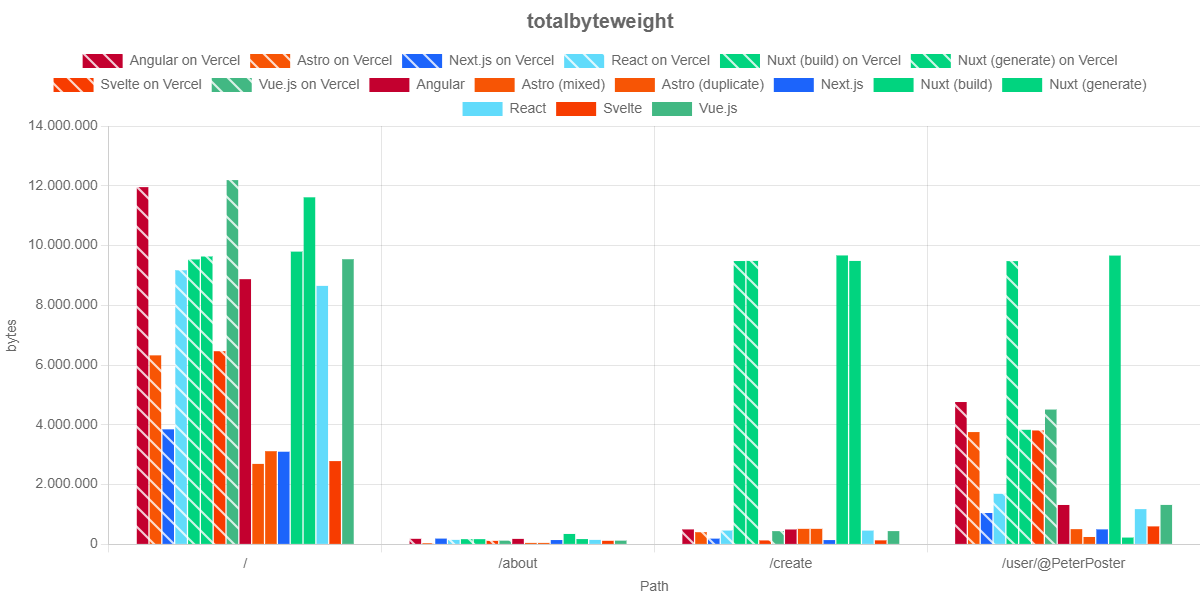
\includegraphics[width=\linewidth, keepaspectratio]{img/lighthouse-results/TBW.png}
    \end{center}
    \caption{\acrfull{tbw}}\label{subfig:LH:totalbyteweight}
  \end{subfigure}
  \begin{subfigure}{0.8\linewidth}
    \begin{center}
      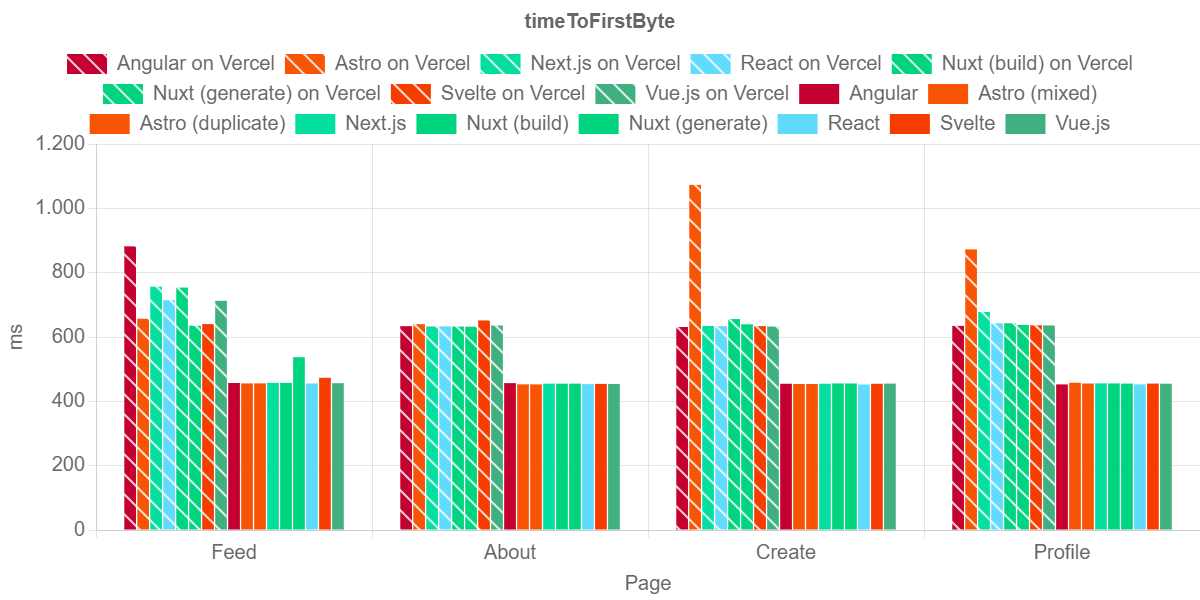
\includegraphics[width=\linewidth, keepaspectratio]{img/lighthouse-results/TTFB.png}
    \end{center}
    \caption{\acrfull{ttfb}}\label{subfig:LH:timeToFirstByte}
  \end{subfigure}
  \begin{subfigure}{0.8\linewidth}
    \begin{center}
      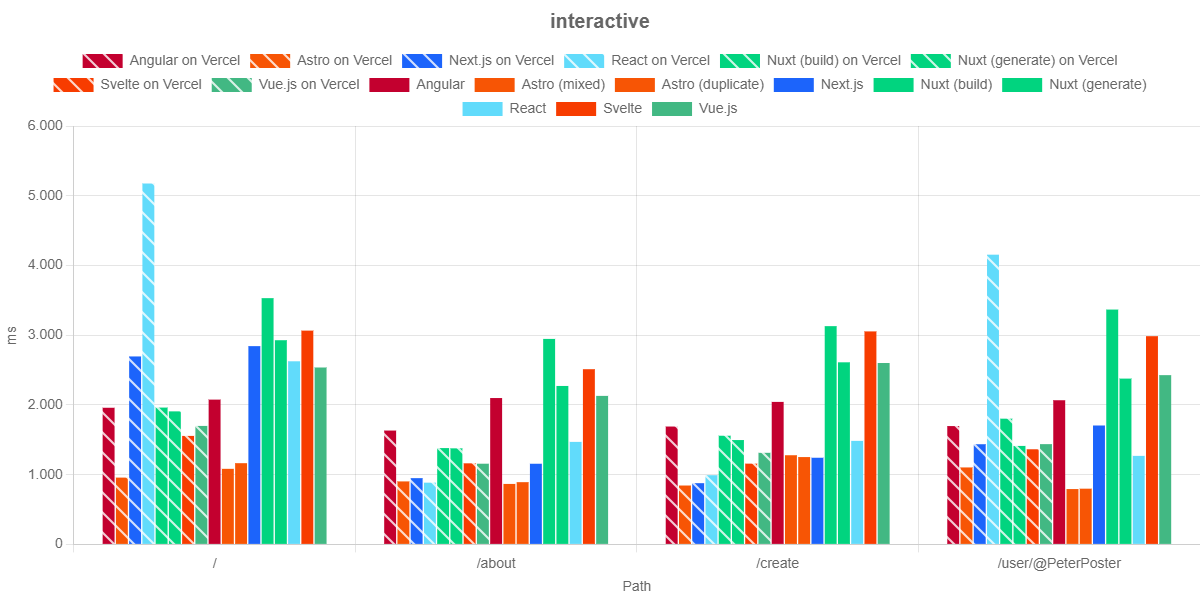
\includegraphics[width=\linewidth, keepaspectratio]{img/lighthouse-results/TTI.png}
    \end{center}
    \caption{\acrfull{tti}}\label{subfig:LH:interactive}
  \end{subfigure}
  \caption{Lighthouse test results in Google Chrome}
\end{figure}
\begin{figure}[ht!]\ContinuedFloat
  \centering  
  \begin{subfigure}{0.8\linewidth}
    \begin{center}
      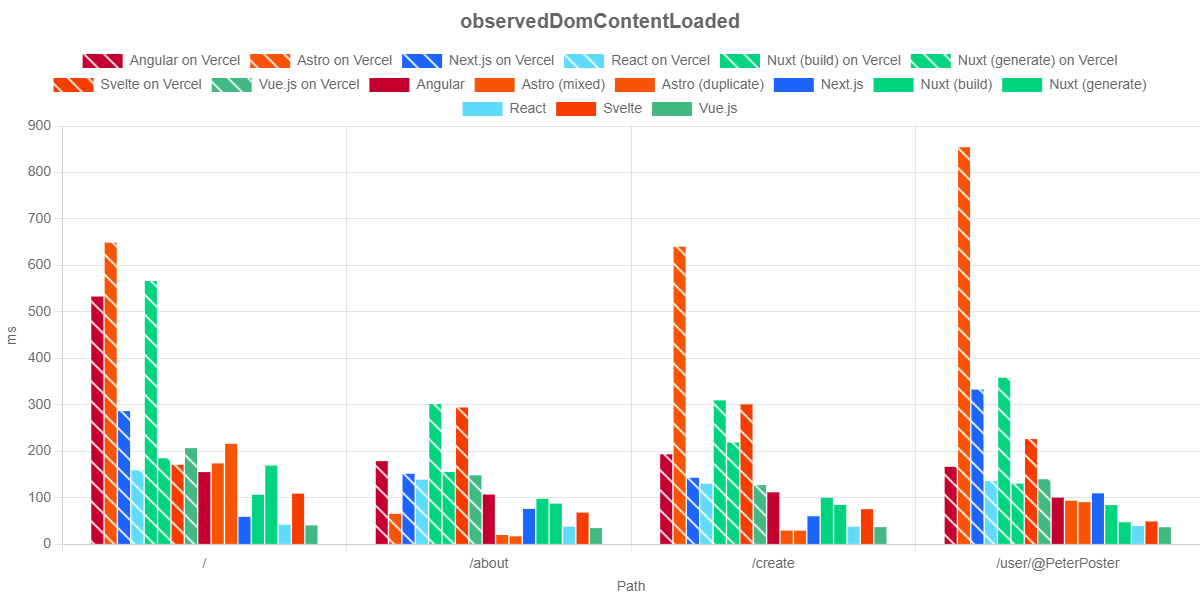
\includegraphics[width=\linewidth, keepaspectratio]{img/lighthouse-results/observedDomContentLoaded.png}
    \end{center}
    \caption{Observed DomContentLoaded}\label{subfig:LH:observedDomContentLoaded}
  \end{subfigure}
  \begin{subfigure}{0.8\linewidth}
    \begin{center}
      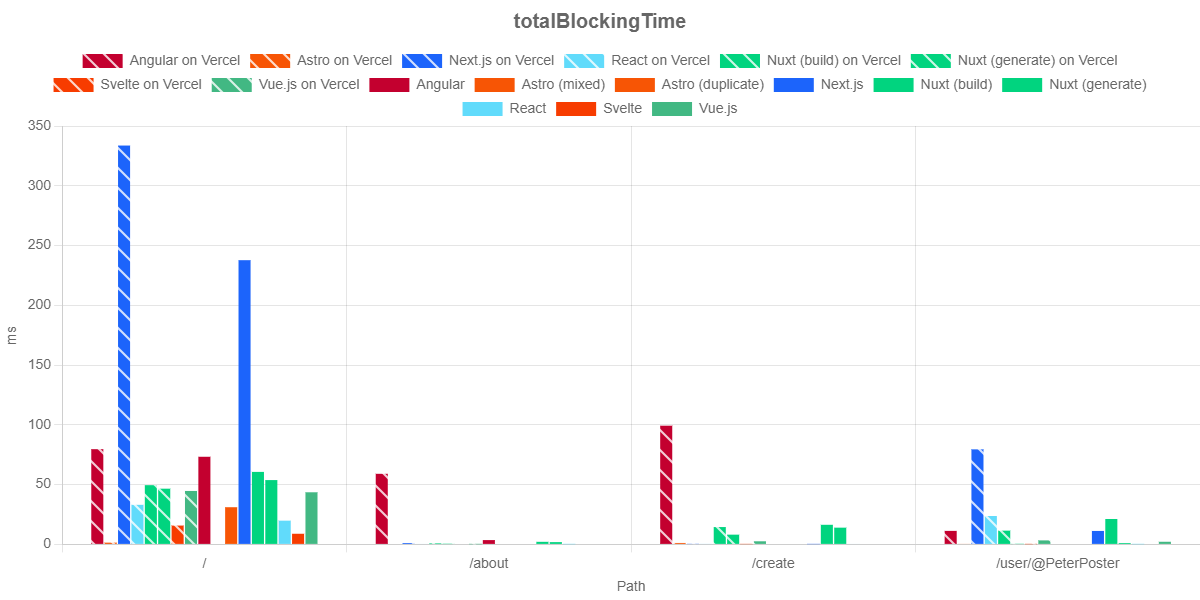
\includegraphics[width=\linewidth, keepaspectratio]{img/lighthouse-results/TBT.png}
    \end{center}
    \caption{\acrfull{tbt}}\label{subfig:LH:totalBlockingTime}
  \end{subfigure}
  \caption{Lighthouse test results in Google Chrome}
\end{figure}
\begin{figure}[ht!]\ContinuedFloat
  \centering
  \begin{subfigure}{0.8\linewidth}
    \begin{center}
      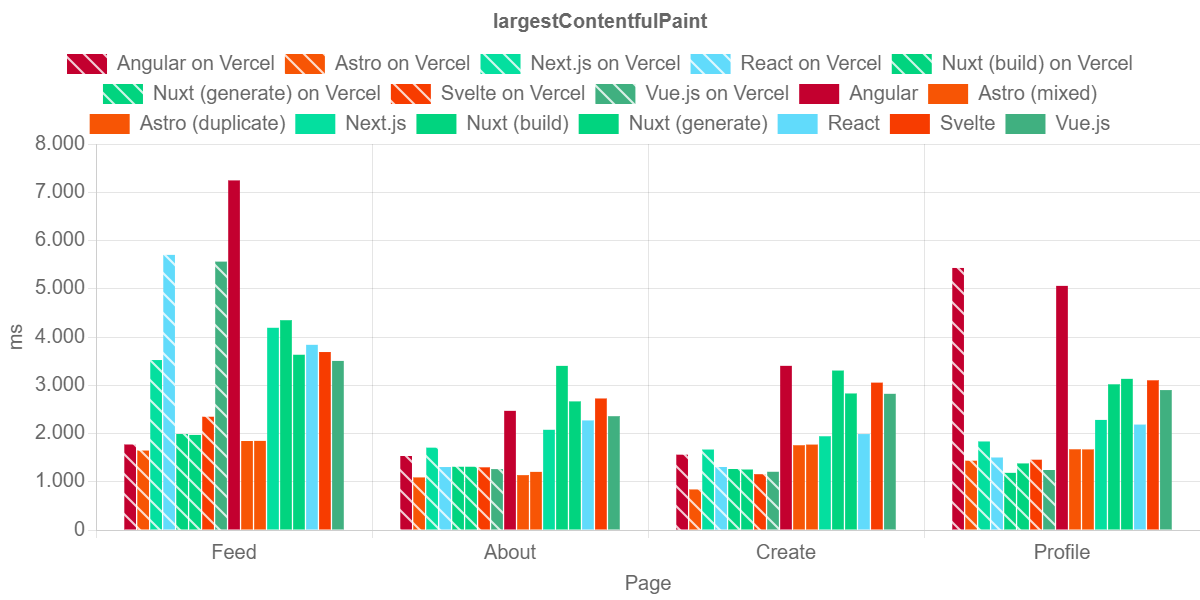
\includegraphics[width=\linewidth, keepaspectratio]{img/lighthouse-results/LCP.png}
    \end{center}
    \caption{\acrfull{lcp}}\label{subfig:LH:largestContentfulPaint}
  \end{subfigure}
  \begin{subfigure}{0.8\linewidth}
    \begin{center}
      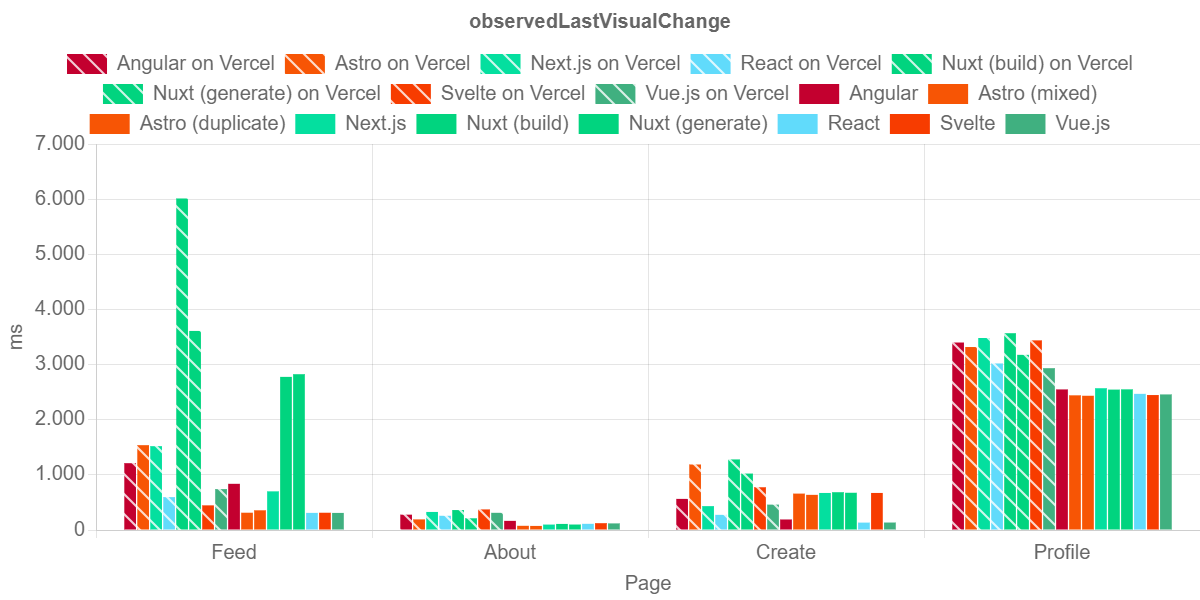
\includegraphics[width=\linewidth, keepaspectratio]{img/lighthouse-results/OLVC.png}
    \end{center}
    \caption{\acrfull{olvc}}\label{subfig:LH:observedLastVisualChange}
  \end{subfigure}
  \caption{Lighthouse test results in Google Chrome}\label{fig:lighthouseResults}
\end{figure}

\textbf{(a)} The \acrlong{tbw} is presented in figure \ref{subfig:LH:totalbyteweight}.
Primarily, the great size of the pages build with Nuxt stand out.
Out of all four pages, this is mainly surprising for the Create page because on initial load only one image has to be loaded.
Yet the Create page and the Profile page appear to be equal in byte size although the latter has decidedly more images on it.
Moreover, the byte size of the Profile page decreases for Nuxt-generate, a characteristic of the two build structures that cannot be found on the Feed page.
The property of Nuxt, that the Create page is as heavy as the Profile page, can be explained through the implementation of the MediaComponent (see listing \ref{lst:Nuxt:MediaComponent:Script}).
All preconfigured image files are imported using \lstinline{import.meta.glob()} (see listing \ref{lst:Nuxt:MediaComponent:Script}, line \ref{line:Nuxt:MediaComponent:imageImport}).
For this reason, the byte size of the page is at least the size of all images on pages that use MediaComponent.
Although this import method is used with Nuxt, Astro and Svelte, Nuxt is the only framework with which this behaviour seems to have this impact.
Secondly, the About page has a small byte size, which is not surprising because it has only one \acrshort{svg} as an image.

In general, pages from Next.js, Astro and Svelte have a small byte weight on the Feed page as well as the Profile page, most likely due to successful image compression.
The byte weight of the Create page and the Profile page is a representation of how well the framework handles selecting which parts of the application have to be loaded.
For the Create page, eight out of the 15 components of the app have to be loaded (nine out of 16 for Astro-duplicate) and five of 15 for the Profile page.
Interestingly, the Create page weighs less than the Profile page for most frameworks except Nuxt.
\\

\textbf{(b)} The measurements of the \acrlong{ttfb} indicate clearly the response time difference from locally hosted applications to applications hosted on Vercel (see figure \ref{subfig:LH:timeToFirstByte}).
To this end, the timings of the About page should be examined.
The difference in \acrshort{ttfb} between local and Vercel lies around 185 ms with local applications responding within 452-457 ms and Vercel responding within 632-651 ms.
Taking this difference as reference for the normal time difference, additional measurements stand out.
Although the local webserver returns the first byte almost equally fast on all paths, Nuxt-generate takes 80 ms longer than its sibling Nuxt-build on the Feed page.
The first response byte is registered 19 ms later on the Feed page with Svelte than the other paths.

On Vercel, the \acrshort{ttfb} fluctuates more between the frameworks.
On the Feed page, the frameworks can be separated into three groups.
Astro, Nuxt-generate and Svelte are the fastest with response times between 635 and 657 ms.
Between 712 and 756 ms lie the times for Next.js, React, Nuxt-build and Vue.js.
Angular has the slowest response time on Vercel and on the Feed page with 882 ms.
The response times on Vercel on the Create page are increased for Astro to 10730 ms by about 430 ms compared to its competitors.
A similar increase is measured on the Profile page with a \acrshort{ttfb} for Astro on Vercel of 872 ms, about 230 ms later than other frameworks.
\\

\textbf{(c)} The \acrlong{tti} of the applications is shown in figure \ref{subfig:LH:interactive}. In contrast to the \acrshort{ttfb}, the \acrshort{tti} is faster on Vercel with the exception of React on the Feed page and both React and Astro on the Profile page.
Possible reasons for this phenomenon include the content encoding, which is missing from local hosting, or simply better traditional webserver performance such as parallelization of request handling on Vercel.
With these faster applications on Vercel, Astro, Svelte, Next.js and Vue.js turn out to be the fastest frameworks for the \acrlong{tti} of the application.
In general, Astro appears to be the framework from which the application has the fastest \acrshort{tti} across pages and hosting environments.
Interestingly, Vue.js, Nuxt, Svelte, Angular and Astro show small fluctuations inbetween pages of 500 ms or less which is relatively little compared to Next.js and React.
\\

\textbf{(d)} Figure \ref{subfig:LH:observedDomContentLoaded} shows the average of observed times of the domContentLoaded event.
Two general characteristics stand out of the data.
First, the timing of the applications that are hosted locally are at least 45 ms earlier than the applications hosted on Vercel.
Second, the observedDomContentLoaded is measured to be much earlier than the \acrshort{ttfb}.
The first observation can be explained by the slower network speed.
The order of \acrshort{ttfb} and observed timing of the domContentLoaded event goes back to throttling not being applied for Lighthouse metrics starting with \enquote{observed} \citep{observedMetrics}.

Astro on Vercel shows the latest domContentLoaded on Vercel except on the About page.
On the other hand, Astro locally shows some of the fastest times on the About page and the Create page.
Angular, Nuxt-build, Next.js and Svelte are the other frameworks with late times for the event.
In contrast, React, Vue.js and Nuxt-generate build applications with earlier event times.
Both measurement characteristics can be explained by the rendering behaviour of the applications.
Astro returns the fully complete \acrshort{dom} in its initial \acrshort{html} document, whereas the frameworks of the second fastest group return half-complete \acrshort{html} documents.
These frameworks demonstrate their rendering capabilities here.
The fastest frameworks for this metric respond to the request with \acrshort{html} skeletons, which naturally results in early domContentLoaded events.
Interestingly, Angular and Nuxt-generate break this pattern.
Angular generates an \acrshort{html} skeleton for all pages that references \acrshort{css} and \acrshort{js} files.
The main difference to Vue.js, for example, is that the \acrshort{js} modules are included in the \acrshort{html} \verb|<body>| for Angular and in the \acrshort{html} \verb|<head>| for Vue.js.
Additionally, all imports are lazy-loading with Vue.js and the scripts for the Angular application are packed into fewer and bigger \acrshort{js} files.
Nuxt-generate on the other hand does not return an empty \acrshort{html} skeleton and is still in the group of fastest frameworks for this metric.
The main difference to other frameworks is that \acrshort{js} files are included in the \acrshort{html} document with \verb|rel="modulepreload"|.
Both of these strategies appear to have a noticeable impact on the timing of the domContentLoaded event.
\\

\textbf{(e)} The results of measurements for the \acrlong{tbt} show drastic differences between the frameworks (see figure \ref{subfig:LH:totalBlockingTime}).
On the one hand, the blocking time is practically negligible for most frameworks on the About, Create and Profile page indicating no unnecessary code execution before rendering.
On the other hand, some frameworks show relatively large \acrshort{tbt}, especially on the Feed page.
Firstly, Astro and Svelte are among the fastest frameworks in the \acrshort{tbt}, although Astro with duplicate components demonstrates a blocking time of 31 ms on the Feed page.
Secondly, the application built with React and Vue.js also have a short blocking time.
Thirdly, Angular produces an application with very low blocking time when hosted locally using the \verb|serve| command, but high blocking time when hosted on Vercel.
The latter two can be explained through an analysis of the scripts and modules loaded and executed on page load.
While Vue.js and React include their scripts in smaller files and only import scripts when needed, Angular bundles \acrlong{js} in fewer and bigger files.
This increases the blocking time, especially for code that is not needed for the page.

The main outlier, however, is Next.js on the Feed and the Profile page.
The \acrshort{tbt} of the application surpasses its next competitor's \acrshort{tbt} by 254 ms on the Feed page on Vercel, 164 ms on the Feed page locally and 56 ms on the Profile page on Vercel.
This is not definitively explainable, but the fact that this effect only greatly affects pages in which images are included using the MediaComponent is an indicator.
Images and videos are loaded using \lstinline|require(`@/assets/stock-footage/${src}`).default|, which is similar to React's \lstinline|require(`src/assets/stock-footage/${src}`)| (see listing \ref{lst:Next:MediaComponent}, line \ref{line:Next:MediaComponent:imageImport} and listing \ref{lst:React:MediaComponent}, line \ref{line:React:MediaComponent:imageImport}).
The interpreted behaviour then is that both applications load the multimedia files synchronously, but Next.js also loads the components synchronously, which results in such a high \acrlong{tbt}.
This would also explain why the effect is less on the local webserver.
\\

\textbf{(f)} Unsurprisingly, the measurements for the \acrfull{olvc} are also in general faster when the application is hosted locally (see figure \ref{subfig:LH:observedLastVisualChange}).
Next.js is the only exception to that on the Create page.
Amongst the frameworks, no clear separation can be identified across the pages or hosting environment, although Vue.js and React are always among the fastest in this metric compared to other frameworks with the same hosting method.
Additionally, Nuxt has the slowest \acrshort{olvc} across pages, especially on the Feed page.
However, the average of Nuxt-build on Vercel is deceiving.
The distribution of the \acrshort{olvc} measurements of Nuxt-build throughout the 20 test repetitions clearly shows that most measurements lie around 4500 ms rather than the average of all values which is 6012 ms.
Nonetheless, the \acrshort{olvc} of Nuxt is still far above the average of other frameworks.
\\

\textbf{(g)} The average measurements for \acrfull{lcp} are shown in figure \ref{subfig:LH:largestContentfulPaint}.
In contrast to other presented metrics, the time of the \acrshort{lcp} is in general earlier for applications hosted on Vercel.
However, both Astro implementations regularly have a faster \acrshort{lcp} locally than other frameworks on Vercel.
Other than that, Angular is the only framework with outlier measurements.
The \acrshort{lcp} measurements are extraordinarily high on the Feed page when hosted locally and on the Profile page independently from the hosting environment.
There is no apparent explanation for either characteristic at this time.

% Page load Playwright tests passes
\begin{table}[!ht]
  \centering
  \begin{tabular}{|l|l|l|}
    \hline
    Angular         & 28/28 \\ \hline
    Astro           & 24/28 \\ \hline
    Next.js         & 28/28 \\ \hline
    Nuxt (build)    & 28/28 \\ \hline
    Nuxt (generate) & 28/28 \\ \hline
    React           & 28/28 \\ \hline
    Svelte          & 24/28 \\ \hline
    Vue.js          & 28/28 \\ \hline
  \end{tabular}
  \caption{Passed Playwright page load tests per framework}
  \label{tab:playwright:pageLoad}
\end{table}

The numbers of passed page load tests with Playwright are listed in table \ref{tab:playwright:pageLoad}.
The only frameworks with which the application does not pass the tests are Astro and Svelte.
For both frameworks the page load budget is exceeded on all four pages when opened in Firefox.
The repetitions of failed tests also exceed the time budget, which causes the tests to be marked as failed.
Figure \ref{subfig:Playwright:loadEventEnd:unbalanced} shows the timings of loadEventEnd across browsers, frameworks and pages, including test repetitions.
It is clear that these test results are outliers compared to other frameworks and browsers.
The load speed in Firefox is slower than the budget only for Astro and Svelte.
Upon inspection of other navigation event times, the reason for this results becomes clear.
The time of requestStart for the failing frameworks in Firefox is already above 2000 ms for all pages.
Interestingly, the timing of this navigation event is not late for all other frameworks.
This differentiating behaviour could not be explained in the time frame of this study.
However, the next step in the analytic process was to inspect a dapted LoadEventEnd metric instead of inspecting the raw measurement of the loadEventEnd.
This balanced loadEventEnd time can be described as

\begin{equation}
\mathit{loadEventEnd}_\mathit{balanced} = \mathit{loadEventEnd}_\mathit{raw} - \mathit{requestStart}
\end{equation}
\vspace{0cm}

Figure \ref{subfig:Playwright:loadEventEnd:balanced} shows the new balanced values.
Using the balanced metric, all pages from all frameworks are loaded within the page load time budgets and the tests should pass.
Still, differences can be found between frameworks and between browsers.
The overview over all results shows four different patterns within a browser.
Unsurprisingly, Chromium and Mobile Chrome as well Desktop Safari and Mobile Safari have similar results.
They differ mainly in the load times of Astro, Svelte and Angular pages.
The third pattern can be found in Microsoft Edge and Google Chrome.
Pages load relatively fast in these two browsers especially with Astro.
The measurements made in Firefox do not resemble the ones made in other browsers.
This might indicate, that its rendering engine \enquote{Gecko} behaves differently to \enquote{Blink} and \enquote{WebKit} which are used in the other browsers.
First, the results are slower on average and it is the only browser in which the load times of React pages fluctuate more than 30 ms inbetween pages.
Second, the fastest times with React are slower than the fastest times with Astro, Nuxt and Vue.js.

\begin{figure}
  \centering
  \begin{subfigure}{\linewidth}
    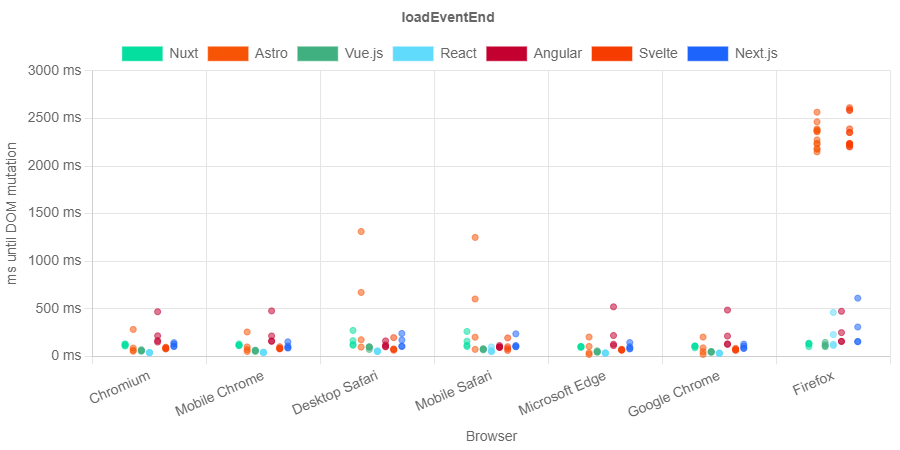
\includegraphics[width=\linewidth, keepaspectratio]{img/playwright-results/loadEventEnd/total.png}
    \caption{unbalanced}\label{subfig:Playwright:loadEventEnd:unbalanced}
  \end{subfigure}
  \begin{subfigure}{\linewidth}
    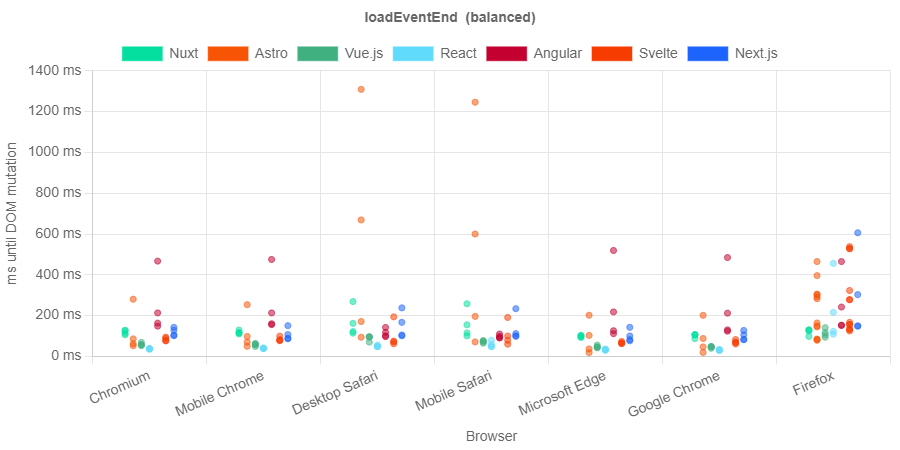
\includegraphics[width=\linewidth, keepaspectratio]{img/playwright-results/loadEventEnd_balanced/total.png}
    \caption{balanced}\label{subfig:Playwright:loadEventEnd:balanced}
  \end{subfigure}
  \caption{Measured loadEventEnd timings}
  \label{fig:Playwright:loadEventEnd}
\end{figure}

As for the frameworks, React is clearly the fastest relating to its loadEventEnd in Chromium, Mobile Chrome, Desktop Safari and Mobile Safari and second fastest in Microsoft Edge and Google Chrome.
Vue.js is second fastest in most browsers and also fluctuates very little. Nuxt, Next.js and Svelte are the next-fastest frameworks across all browsers.
Angular is one of the slowest frameworks for most pages and browsers except some measurements of Astro.
The fastest or the slowest measured times are measured with Astro depending on the browsers, but always fluctuate relatively much compared to other frameworks.


\subsection{Component Load Times}\label{subsec:componentloadtimes}
% 1. Which components load with delay?
% 2. Which frameworks have fast-loading delayed components?
% 3. Do pre-rendered pages even have delayed components?

The load time of components is an indicator for how well frameworks split resources for the load of their applications between part of the pages.
The relevant metrics for the component load are \acrfull{olvc}, \acrfull{tbt}, \acrfull{tti}, the timing of loadEventEnd, \acrfull{ofvc} and the measured \acrshort{dom} mutation times immediately after the initial page load.
To measure these metrics, the tests are executed as described previously and documented as described in section \ref{subsec:pageloadtimes}.
The same rules for the presentations of the results apply in this section.

Because the same time frame is inspected as in the previous section, the relevant metrics \acrshort{tbt}, \acrshort{olvc}, \acrshort{tti} and balanced loadEventEnd can be used to analyze the behaviour of component load (see figures \ref{subfig:LH:totalBlockingTime}, \ref{subfig:LH:interactive}, \ref{subfig:LH:observedLastVisualChange} and \ref{subfig:Playwright:loadEventEnd:balanced}).
However, no new interpretations can be taken for component load times because every measurement that includes the complete page load might or might not be caused by slowly loading components.
Therefore, failed tests due to the time budget being exceeded cannot be unequivocally attributed to either slow network speeds, browser behaviour, client behaviour, the used framework or single components.
Additional metrics are needed to identify component load times.

The \acrshort{ofvc} is the time after which the first visual change is made within the viewport (see figure \ref{subfig:LH:observedFirstVisualChange}).
It can be either the time after which prerendered \acrshort{html} elements appear or the time after which an empty \acrshort{dom} gets filled through \acrshort{js} and visual changes are made.
The measurements of the \acrshort{ofvc} show that, in general, the first visual change is earlier for locally hosted applications, which is unsurprising because the resources load earlier.
Frameworks with an early \acrshort{ofvc} are Astro, React and Next.js with the only exception being Astro on Vercel on the Create page.
The Angular application on the other hand displays late \acrshort{ofvc} values compared to its competitors locally.
On Vercel, Nuxt-build has relatively late values across all pages.

% REVIEW: write more interpretation about the results

% OVCD
\begin{figure}[ht!]
  \centering
  \begin{subfigure}{0.95\linewidth}
    \begin{center}
      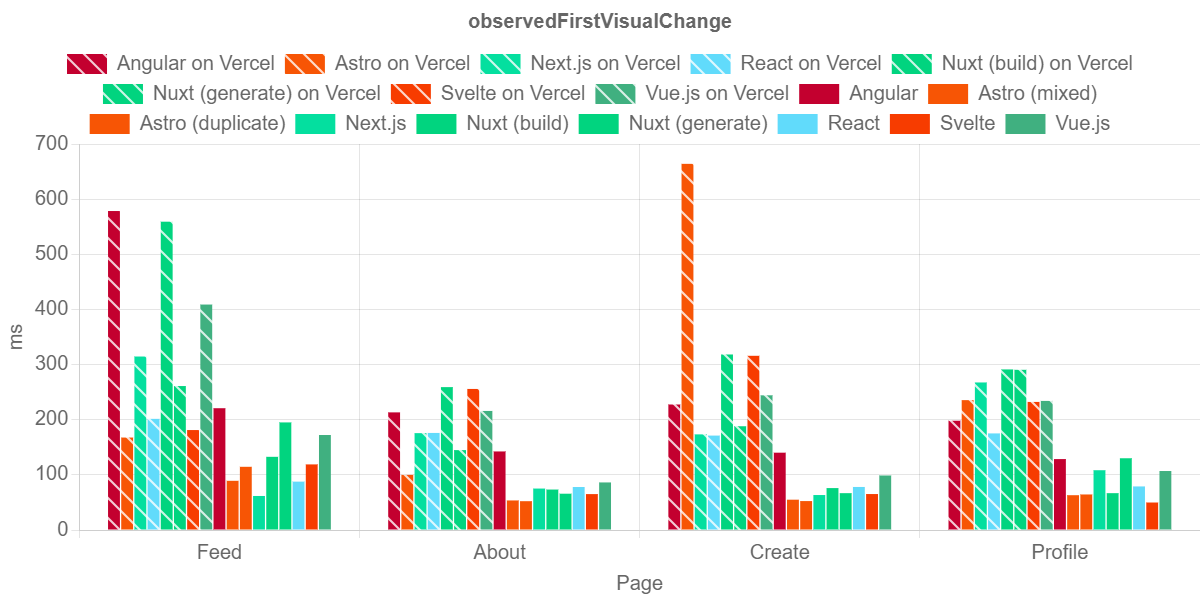
\includegraphics[width=\linewidth, keepaspectratio]{img/lighthouse-results/OFVC.png}
    \end{center}
    \caption{\acrfull{ofvc}}
    \label{subfig:LH:observedFirstVisualChange}
  \end{subfigure}
  \begin{subfigure}{0.95\linewidth}
    \begin{center}
      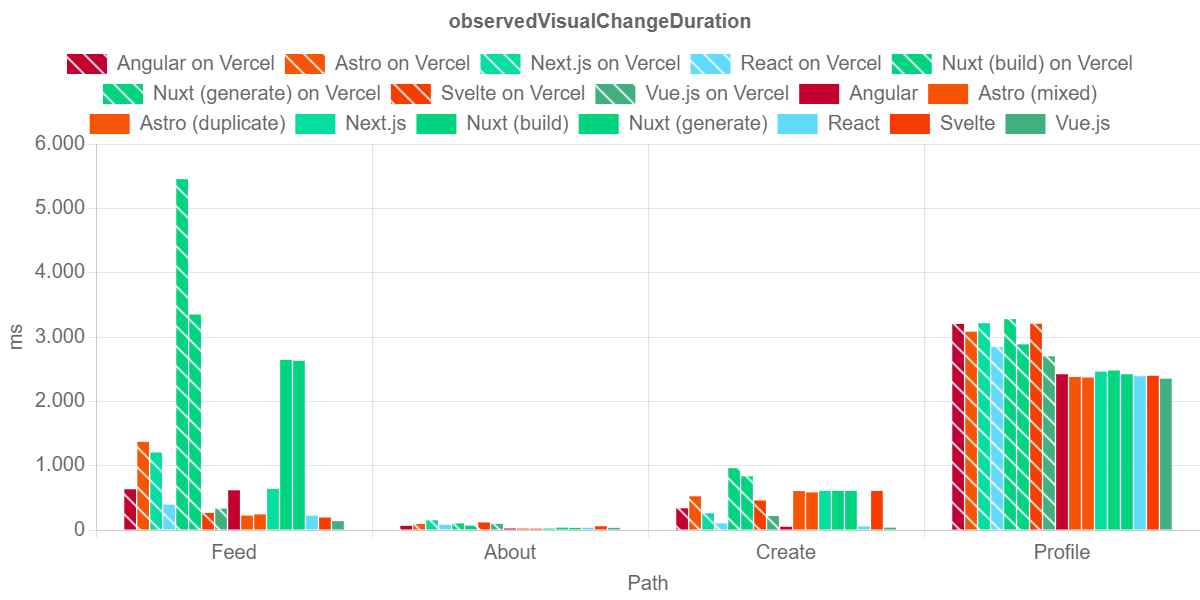
\includegraphics[width=\linewidth, keepaspectratio]{img/lighthouse-results/olvc-ofvc.png}
    \end{center}
    \caption{\acrfull{ovcd}}\label{subfig:LH:observedVisualChangeDuration}
    \label{fig:LH:OVCD}
  \end{subfigure}
  \caption{\acrfull{ofvc} (\subref{subfig:LH:observedFirstVisualChange}) and \acrfull{ovcd} (\subref{subfig:LH:observedVisualChangeDuration})}
\end{figure}

More interesting than the raw \acrshort{olvc} and \acrshort{ofvc} values is the difference between the measurements.
This thesis defines a new metric \enquote{Observed Visual Change Duration}.
It shows the time after the first visual mutation to the page has been bade until the last visual change.
It is simply deferred from the \acrshort{olvc} and \acrshort{ofvc} and is defined as

\begin{multline}
  \mathit{observedVisualChangeDuration} =\\ \mathit{observedLastVisualChange} - \mathit{observedFirstVisualChange}
\end{multline}
\vspace{0cm}

Figure \ref{fig:LH:OVCD} shows the resulting values for the \acrfull{ovcd} from this study.
The great difference between locally tested applications and applications on Vercel means that visual changes, especially the last, are dependent on network delay or \acrlong{js} execution speed.
Vue.js, React and Angular produce low \acrshort{ovcd} measurements except on the Profile page.
This is even the case if the \acrshort{ofvc} is late.
The reason for this result is that no visual changes are made to the page until the \acrshort{html} and \acrshort{js} is parsed and executed.
This stands in contrast to prerendered, server-side rendered or semi-rendered pages.
With these pages, the first visual update can already be made after only the \acrshort{html} is parsed.
Therefore \acrshort{csr} frameworks can achieve faster \acrshort{ovcd} values on the pages without components that have differently fast loading components.
Notably, the Profile page is an outlier among the pages.
This is because the static header of the page can be displayed as soon as possible, but the rest of the page needs two additional service functions to finish before images and videos can be loaded.
The effect of those chained \acrlong{js} executions can clearly be identified using the \acrshort{ovcd}.

% Playwright Page load mutations
\begin{figure}[ht!]
  \centering
  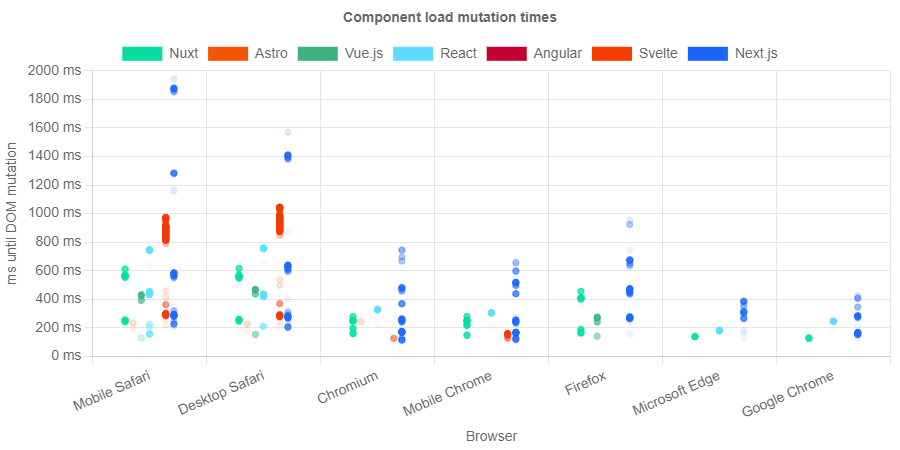
\includegraphics[width=\linewidth, keepaspectratio]{img/playwright-results/pageLoadMutations/total.png}
  \caption{Component load mutation times}
  \label{fig:Playwright:pageLoadMutations:total}
\end{figure}

Figure \ref{fig:Playwright:pageLoadMutations:total} shows the \acrshort{dom} mutation times of elements that were registered through Playwright right after the initial page load.
Primarily, the most noticeable result of these measurements is that some results appear to be missing.
For example, there are no measurements from the Angular application at all.
The reason for missing measurements could be that all \acrshort{dom} mutations have taken place before the MutationObserver could be initialized because the injection of the recording script through Playwright takes longer than the page load or all changes take place before the first interval of 100 ms (see listing \ref{lst:performance-recorder}, line \ref{line:mutationInterval}).
The other possible reason for this phenomenon could be that mutations are slower than the manually defined recording time of ten seconds (see listing \ref{lst:dynamic-performance-spec}, line \ref{line:dynamic-performance-spec:maxTime}), but it is less likely because no mutation is recorded to be over 1900 ms with any browser, page or framework.
Therefore, missing recordings indicate the framework is either loading too fast or too slow to record \acrshort{dom} mutations.
In addition, other results match the interpretation (see section \ref{subsec:componentupdatetimes}).
Because the applications have differences in the \acrshort{dom} structure and render time, the number of mutations fluctuates naturally.
Adjusting for possible variations here, four frameworks seem to have missing measurements.
The applications built with Angular (no mutations), Astro (11 mutations), Vue.js (174 mutations) and React (527 mutations) have surprisingly few mutations.
The applications built with Nuxt (1011 mutations), Next.js (1654 mutations) and Svelte (1857 mutations) have over 1000 mutations.
Although the latter numbers could indicate full recording coverage of the mutations, the distribution of recordings between browsers and pages prove that not all mutations were recorded, even with these latter three frameworks.
For example, no mutations were recorded on the About page with Nuxt and Next.js.
In fact, Svelte is the only framework with which mutations were recorded on the About page, but only in Mobile Chrome, Chromium, Mobile Safari and Desktop Safari.
Then again, there are apparently no mutations with Svelte on the Profile page in any browser.

Although the missing data prevents some unambiguous comparisons between frameworks, the presence of some recordings indicates load speed differences between frameworks and browsers.
First, many relatively late recordings could be made in Desktop Safari and Mobile Safari.
This indicates that the method of measurement results in slow \acrshort{dom} mutation times in these browsers, especially with Svelte and Next.js.
Additionally, in Microsoft Edge and Google Chrome only very few measurements could be made, so the two browsers can be considered especially fast for this measurement method.
Second, Next.js appears to be the slowest of the frameworks in this metric.
Svelte also demonstrates slow mutations, but only in Desktop Safari and Mobile Safari.
The other frameworks that appear in the summary of mutations, Nuxt, React and Vue.js, also have some relatively high recorded mutation times, but all recorded times are below 760 ms.
With these frameworks, the most interesting observation is that not only are the mutation times faster with Microsoft Edge and Google Chrome, but they are also more bundled together than with other browsers.

The last possible observation from the data is that no mutation time is below 100 ms.
The implementation of the MutationObserver is the reason for this.
Because the start time is defined immediately and the interval callback is executed first after a 100 ms delay, no mutation times below 100 ms can be recorded.
Changing the implementation to an interval of 20 ms and executing the initialization function once immediately does allow for earlier recording times for few frameworks.
The tested applications built with Astro, Next.js, React, Svelte and Vue.js then have recorded mutation times below 100 ms.
The earliest recorded time with the 20 ms interval is 41 ms with Vue.js on the About page in Microsoft Edge.
Naturally, the number of recordings also increases drastically for all frameworks except Angular.
42 mutations with Astro, 640 mutations with Vue.js, 1309 mutations with Nuxt, 1704 mutations with React, 2260 mutations with Next.js and 6412 mutations with Svelte were recorded.
The increase in early recordings and the minimum times per framework support two interpretations relating to the interval time.
First, quick initialization intervals do make the recording more complete because fewer fast mutations are not recorded.
If these fast mutations are required to be present in the test or its report, then decreasing the interval speed is a requirement.
Second, the minimal time becomes dependent on the initialization behaviour and speed.
The presence of fast data points for some frameworks cannot be definitively traced back to the framework being faster than others because fast data points might still be missing for other frameworks due to unreliable injection behaviour.
In addition, rapid initialization attempts require more resources and therefore might actually decrease the performance of any code execution or rendering.
For these reasons, the configuration of a initialization interval is a balance between the completeness of \acrshort{dom} mutation recordings and comparability of fast mutations.

\subsection{Component Update Times}\label{subsec:componentupdatetimes}
% 1. Which differences can be made out towards [Component update times](#component-update-times)?
% 2. Which HTML-Elements even update?
% 3. Which frameworks update HTML-Elements faster than others?

Section \ref{subsec:tests} defines the update time of a component using the user input time and the time of the \acrshort{dom} mutation.
Only the mutation times were used in this study to keep the method of measurement valid for as many applications frameworks as possible.
Because the user input action is delayed and the zero-time is reset beforehand (see listing \ref{lst:state-change-spec}, lines \ref{line:actionDelay} - \ref{line:userAction}), the punctual initialization of the MutationObserver is not an issue when testing \acrshort{dom} mutations triggered by user inputs (as described in section \ref{subsec:componentloadtimes}).

The number of mutation types to the \acrshort{dom} per user action are displayed in table \ref{tab:mutations:total}.
It is clear that the frameworks can be split into three distinct groups by number of different mutations.
This list intentionally does not count identical mutations such as appending another element to the list of \verb|<span>| elements in the post caption of the preview.
Angular and Next.js make the most changes to the \acrshort{dom} during the user actions with 14 and 15 recorded mutations, respectively.
Then, both Astro and React have a similar number of mutations with nine mutations in total.
This similarity is not surprising because the Astro island of the CreateForm consists of identical React components to the pure React application.
The group of frameworks with the least \acrshort{dom} mutations changes on six different elements in the \acrshort{dom} in total.
They are Nuxt, Vue.js and Svelte.
Tables \ref{tab:mutations:captionChange}, \ref{tab:mutations:mediaSelection}, \ref{tab:mutations:mediaSourceInsertion} and \ref{tab:mutations:postCreation} list the \acrshort{html} elements that were mutated after user input for all four user actions.
Surprisingly, the grouping of the frameworks does not translate directly to the specific mutated elements.
In general, each described group does update similar elements with similar mutations, but they are not exact copies of each other in this regard.

% Total user action mutations
\begin{table}[!ht]
  \centering
  \begin{adjustbox}{angle=90}
    \begin{tabular}{|l|r|r|r|r|r|r|r|}
      \hline
      ~                       & \textbf{Angular}  & \textbf{Astro}  & \textbf{Next.js}  & \textbf{Nuxt} & \textbf{React}  & \textbf{Vue.js} & \textbf{Svelte} \\ \hline
      Caption change          & 3                 & 2               & 3                 & 1             & 2               & 1               & 1               \\ \hline
      Media selection         & 3                 & 1               & 3                 & 1             & 1               & 1               & 1               \\ \hline
      Media source insertion  & 3                 & 2               & 3                 & 1             & 2               & 1               & 1               \\ \hline
      Post creation           & 5                 & 4               & 6                 & 3             & 4               & 3               & 3               \\ \hline\hline
      \textbf{Total}          & 14                & 9               & 15                & 6             & 9               & 6               & 6               \\ \hline
    \end{tabular}
  \end{adjustbox}
  \caption{Total number of \acrshort{dom} mutation types per framework and user action}
  \label{tab:mutations:total}
\end{table}

Figure \ref{fig:playwrightResults:total} presents the mutation times of each framework per browser with all recorded times across user actions.
The first results for this study is that almost all frameworks do finish mutating the \acrshort{dom} within the predefined time budget of 500 ms.
Slower mutations do speed up in test repetitions.
As a result, the Playwright tests pass.
In addition, the maximum time for mutations is decidedly dependent on the browser.
While Desktop Safari apparently is the slowest browser for \acrshort{dom} mutations triggered by the user, especially with Next.js, almost all mutations in Chromium, Microsoft Edge and Google Chrome even finish within the time limit for earliest mutations of 100 ms.
Mobile Chrome also shows the same characteristics with the exception of some mutations by Svelte and Next.js after the Post Creation action.

% Playwright results
\begin{figure}[t]
  \centering
  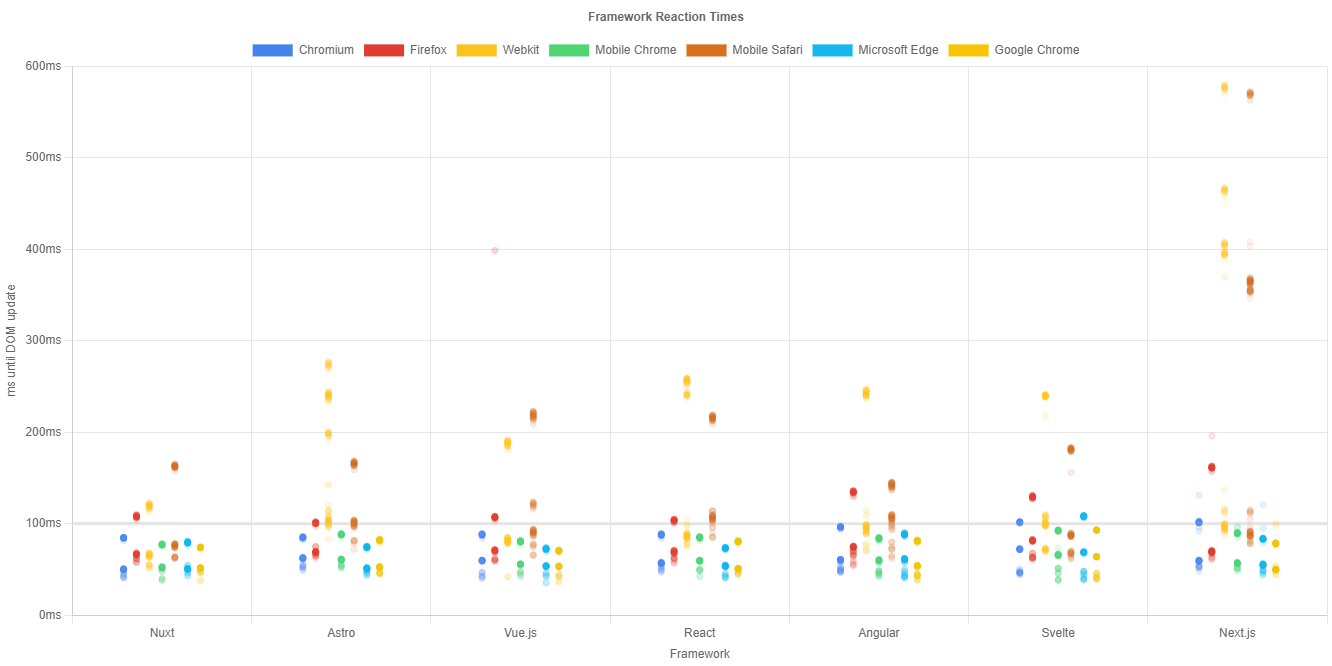
\includegraphics[width=\linewidth, keepaspectratio]{img/playwright-results/userActions_byUserAction/total.png}
  \caption{Recorded \acrshort{dom} mutation timings after user actions}
  \label{fig:playwrightResults:total}
\end{figure}

% Playwright results per framework (user actions)
\begin{figure}[ht!]
  \centering
  \begin{subfigure}{0.8\linewidth}
    \begin{center}
      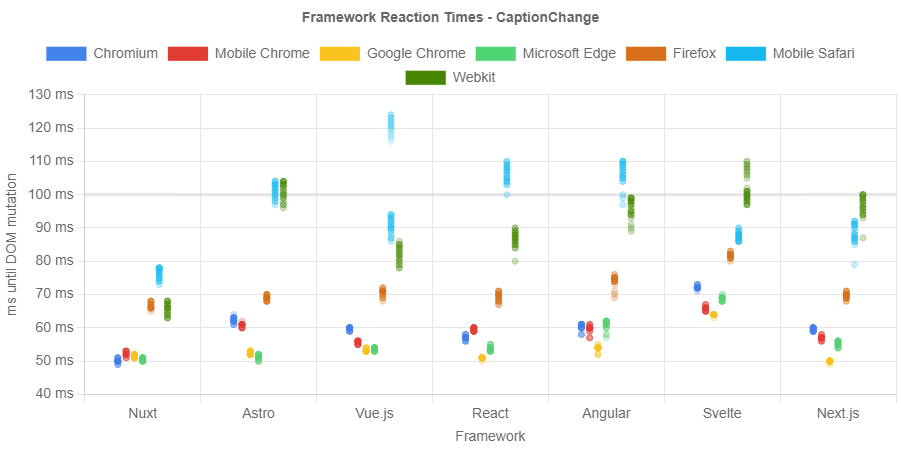
\includegraphics[width=\linewidth, keepaspectratio]{img/playwright-results/userActions_byUserAction/captionChange.png}
    \end{center}
    \caption{Mutations after Caption Change}\label{subfig:PW:captionChange}
  \end{subfigure}
  \begin{subfigure}{0.8\linewidth}
    \begin{center}
      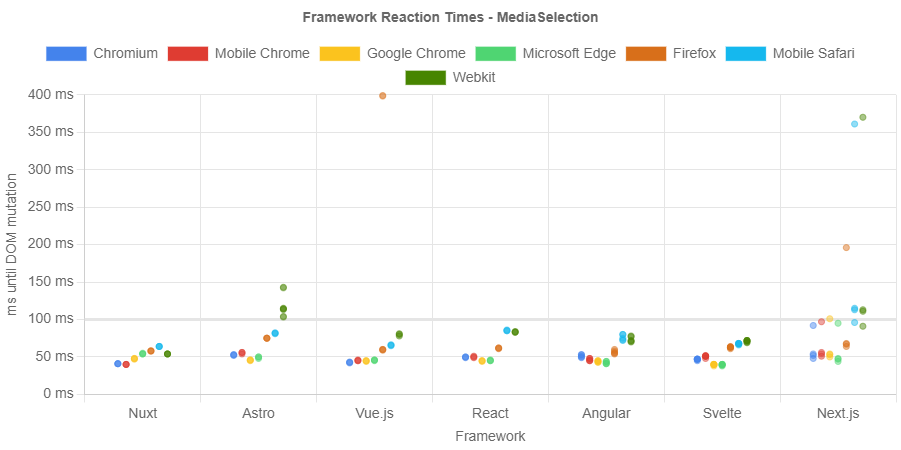
\includegraphics[width=\linewidth, keepaspectratio]{img/playwright-results/userActions_byUserAction/mediaSelection.png}
    \end{center}
    \caption{Mutations after Media Selection}\label{subfig:PW:mediaSelection}
  \end{subfigure}
  \begin{subfigure}{0.8\linewidth}
    \begin{center}
      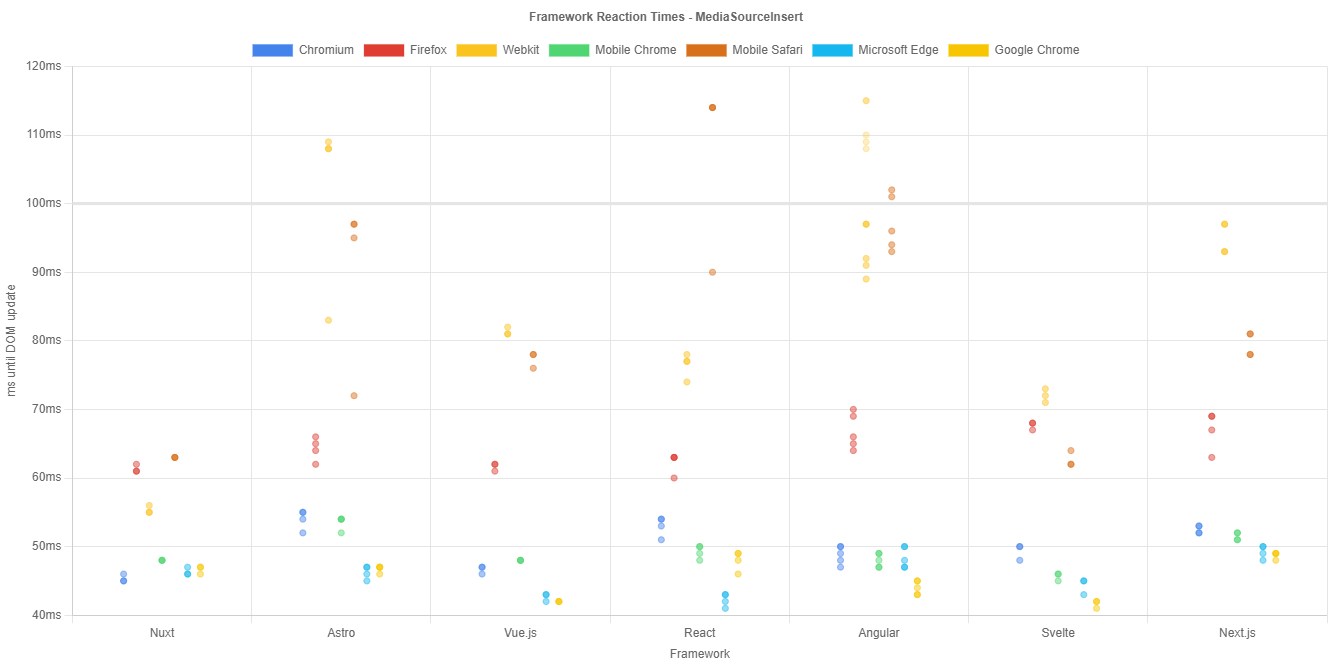
\includegraphics[width=\linewidth, keepaspectratio]{img/playwright-results/userActions_byUserAction/mediaSourceInsert.png}
    \end{center}
    \caption{Mutations after Media Source Insert}\label{subfig:PW:mediaSourceInsert}
  \end{subfigure}
  \caption{Recorded \acrshort{dom} mutation timings per framework}
\end{figure}
\begin{figure}[ht!]\ContinuedFloat
  \centering
  \begin{subfigure}{0.8\linewidth}
    \begin{center}
      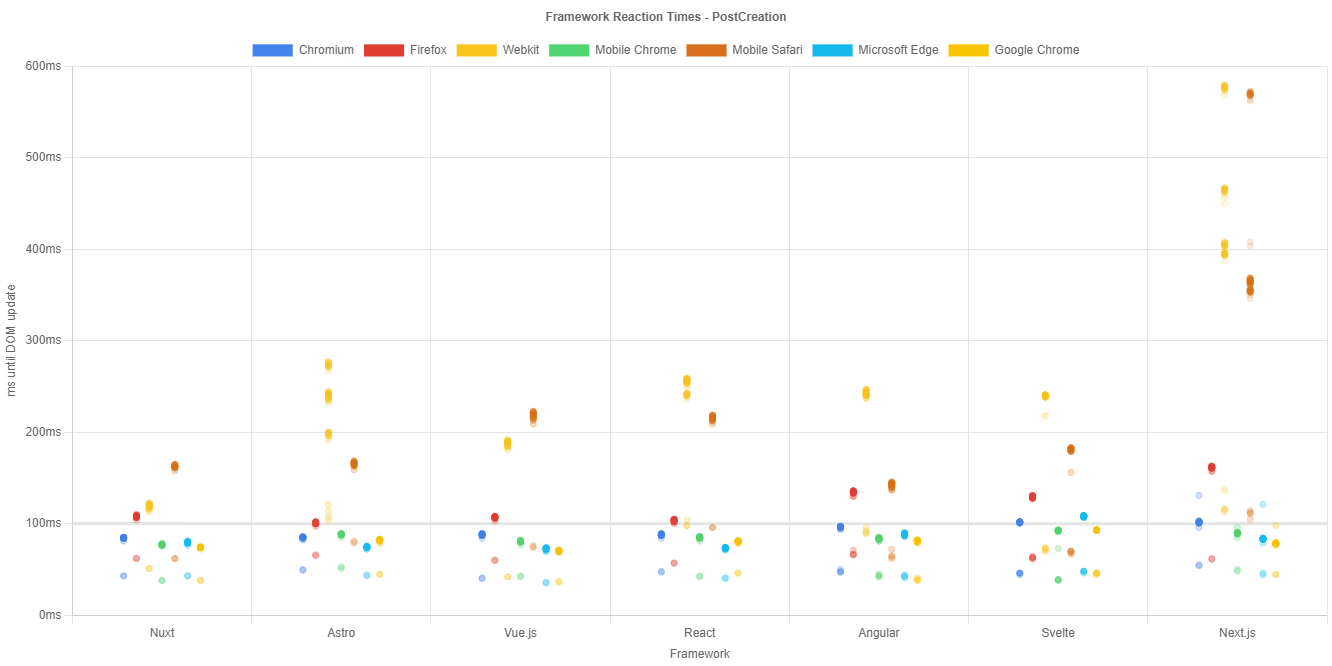
\includegraphics[width=\linewidth, keepaspectratio]{img/playwright-results/userActions_byUserAction/postCreation.png}
    \end{center}
    \caption{Mutations after Post Creation}\label{subfig:PW:postCreation}
  \end{subfigure}
  \caption{Recorded \acrshort{dom} mutation timings per framework}
  \label{fig:playwrightResults:frameworks}
\end{figure}

Figure \ref{fig:playwrightResults:frameworks} contains the update times of the four user actions per browser and framework.
A few generalizations are possible to extract from these results.
For the Caption Change (see figure \ref{subfig:PW:captionChange}), Nuxt appears to be the fastest framework on all browsers except on Google Chrome where Next.js makes faster \acrshort{dom} mutations.
Astro is also a relatively fast framework in Microsoft Edge and Google Chrome, but is is one of the slowest frameworks in Desktop Safari and Mobile Safari.
In general, Nuxt, Next.js, Vue.js, React and Angular make \acrshort{dom} mutations in under 70 ms in Chromium, Mobile Chrome, Microsoft Edge and Google Chrome.
Svelte on the other hand is apparently the slowest framework for this user action on average.
The recorded \acrshort{dom} mutation times for Media Selection can be found in figure \ref{subfig:PW:mediaSelection}.
Most of the mutations are below the 100 ms time limit with only few exceptions.
Astro is slower than the limit in Desktop Safari, Next.js is slower in Google Chrome, Mobile Safari and Desktop Safari and Vue.js has an outlier measurement in Firefox.
Here, Nuxt, Vue.js, React, Angular and Svelte have similarly well to each other.
Apart from the mentioned outliers, the results from these frameworks lie between 38 and 85 ms.
The measurements for the Media Source Insert action are very similar to the Media Selection action (see figure \ref{subfig:PW:mediaSourceInsert}).
Again, Nuxt performs very fast in all browsers and all frameworks are somewhat similar to each other except in Firefox, Mobile Safari and Desktop Safari.
The latter two are again the slowest browsers on average and Firefox is the third slowest.
In these browsers, Nuxt and Svelte are the fastest frameworks.
The Post Creation action is the slowest user action to finish (see figure \ref{subfig:PW:postCreation}), which is unsurprising because it is combined from two other actions.
It is therefore impossible to finish faster than either single user action.
The update times for each user action can even be seen in two distinct groupings in the recordings.
For this action, Next.js is clearly the slowest framework in relation to its competitors, but this difference is only significant on Desktop Safari and Mobile Safari.

Across all user actions, applications mutate the \acrshort{dom} slowest in Mobile Safari and Desktop Safari, closely followed by Firefox.
The other browsers Chromium, Mobile Chrome, Google Chrome and Microsoft Edge lie very close to each other and the average mutations times differ from each other at a maximum of 15 ms.

Table \ref{tab:mutations:times} lists the minimal and maximal mutation times of the frameworks in each browser, as well as the mean average for each combination.
In addition, the mean average and weighted averages of all minima, maxima and averages of mutation times in each framework are calculated.
The weighted averages are based on the usage percentages of browsers (see table \ref{tab:browserUsage}).
These results indicate clearly that Next.js produces the slowest mutations both on average and weighted average.
In contrast, Nuxt makes the fastest updates across browsers.
Then, Angular comes in second, Vue.js is third and React is the fourth-fastest framework.
The second-slowest framework on average is Astro, but it comes in faster than Svelte in the ranking of frameworks when the weights are calculated in.


% browser usage
\begin{table}[!h]
  \centering
  \begin{tabular}{|l|r|}
    \hline
    \textbf{Browser}  & \textbf{Usage quota} \\ \hline
    Google Chrome     & 65.68 \% \\ \hline
    Desktop Safari    & 17.96 \% \\ \hline
    Microsoft Edge    & 5.26 \% \\ \hline
    Firefox           & 2,75 \% \\ \hline
    Chromium          & NA \\ \hline
    Mobile Chrome     & NA \\ \hline
    Mobile Safari     & NA \\ \hline
  \end{tabular}
  \caption{Browser usage \citep{browserUsage}}
  \label{tab:browserUsage}
\end{table}

\pagebreak

% DOM Mutation times state change
\begin{table}[h!]
  \centering
  {
  \footnotesize
  \begin{adjustbox}{angle=90}
    {
      \rowcolors{1}{lightgray!40!}{lightgray!40!}
      \begin{tabular}{|l|c|c|c|c|c|c|c|c|}
        \hline
        ~                                            & \textbf{Angular} & \textbf{Astro}                  & \textbf{Next.js}               & \textbf{Nuxt}           & \textbf{React} & \textbf{Svelte} & \textbf{Vue.js} & \textbf{Framework Avg.}  \\ \hline
\rowcolor{white}                                     & 44               & 51                              & 47                             & 39                      & 44             & 38              & 51              & 45                \\
\rowcolor{white}                                     & \textbf{69}      & \textbf{71}                     & \textbf{75}                    & \textbf{66}             & \textbf{58}    & \textbf{74}     & \textbf{77}     & \textbf{70}       \\
\rowcolor{white} \multirow{-3}{*}{Chromium}          & 95               & 89                              & 108                            & 94                      & 85             & 95              & 104             & 96                \\ \hline
                                                     & 54               & 63                              & 59                             & 59                      & 54             & 60              & 52              & 57                \\
                                                     & \textbf{89}      & \textbf{99}                     & \textbf{142}                   & \textbf{83}             & \textbf{84}    & \textbf{94}     & \textbf{82}     & \textbf{96}       \\
                 \multirow{-3}{*}{Firefox}           & 123              & 142                             & 235                            & 108                     & 181            & 129             & 103             & 146               \\ \hline
\rowcolor{white}                                     & 77               & \cellcolor{red!50}87            & 79                             & 51                      & 84             & 70              & 47              & 71                \\
\rowcolor{white}                                     & \textbf{123}     & \textbf{170}                    & \cellcolor{red!50}\textbf{304} & \textbf{86}             & \textbf{169}   & \textbf{164}    & \textbf{136}    & \textbf{164}      \\
\rowcolor{white} \multirow{-3}{*}{Desktop Safari}    & 172              & 270                             & \cellcolor{red!50}493          & 124                     & 280            & 283             & 200             & 260               \\ \hline
                                                     & 44               & 49                              & 47                             & 42                      & 44             & 45              & 46              & 45                \\
                                                     & \textbf{67}      & \textbf{69}                     & \textbf{94}                    & \textbf{61}             & \textbf{67}    & \textbf{81}     & \textbf{69}     & \textbf{73}       \\
                 \multirow{-3}{*}{Mobile Chrome}     & 90               & 85                              & 143                            & 82                      & 82             & 116             & 89              & 98                \\ \hline
\rowcolor{white}                                     & 52               & 78                              & 73                             & 47                      & 67             & 56              & 52              & 61                \\
\rowcolor{white}                                     & \textbf{106}     & \textbf{154}                    & \textbf{196}                   & \textbf{110}            & \textbf{126}   & \textbf{126}    & \textbf{133}    & \textbf{136}      \\
\rowcolor{white} \multirow{-3}{*}{Mobile Safari}     & 152              & 254                             & 372                            & 167                     & 183            & 208             & 206             & 220               \\ \hline
                                                     & 43               & 44                              & 46                             & 37                      & 41             & 40              & 40              & 42                \\
                                                     & \textbf{70}      & \textbf{64}                     & \textbf{73}                    & \textbf{61}             & \textbf{62}    & \textbf{74}     & \textbf{61}     & \textbf{67}       \\
                 \multirow{-3}{*}{Microsoft Edge}    & 90               & 80                              & 134                            & 85                      & 75             & 102             & 79              & 93                \\ \hline
\rowcolor{white}                                     & 41               & 43                              & 41                             & \cellcolor{green!50}34  & 40             & 39              & 37              & 39                \\
\rowcolor{white}                                     & \textbf{62}      & \cellcolor{green!50}\textbf{57} & \textbf{69}                    & \textbf{60}             & \textbf{59}    & \textbf{64}     & \textbf{61}     & \textbf{62}       \\
\rowcolor{white} \multirow{-3}{*}{Google Chrome}     & 84               & \cellcolor{green!50}72          & 99                             & 77                      & 77             & 89              & 77              & 82                \\ \hline
                 \hline
                                                     & 51               & 59                              & 56                             & 44                      & 53             & 50              & 46              & ~                 \\
                                                     & \textbf{84}      & \textbf{98}                     & \textbf{136}                   & \textbf{75}             & \textbf{89}    & \textbf{97}     & \textbf{88}     & ~                 \\
                 \multirow{-3}{*}{Browser Avg.}      & 115              & 142                             & 226                            & 105                     & 138            & 146             & 123             & ~                 \\ \hline
\rowcolor{white}                                     & 45               & 48                              & 45                             & 35                      & 45             & 42              & 36              & ~                 \\
\rowcolor{white}                                     & \textbf{69}      & \textbf{74}                     & \textbf{107}                   & \textbf{60}             & \textbf{75}    & \textbf{78}     & \textbf{70}     & ~                 \\
\rowcolor{white} \multirow{-3}{*}{Weighted Br. Avg.}  & 94               & 103                             & 167                            & 80                      & 110            & 118             & 93              & ~                 \\ \hline
      \end{tabular}
      }

    \end{adjustbox}

    \vspace{0.5cm}
      
    {\rowcolors{1}{lightgray!40!}{lightgray!40!}
    
      \begin{tabular}{|l|c|}
        \hline
      ~ & Framework \\ \hline
      \rowcolor{white}                            & minimum with framework in browser \\
      \rowcolor{white}                            & \textbf{average with framework in browser} \\
      \rowcolor{white} \multirow{-3}{*}{Browser}  & maximum with framework in browser \\ \hline \hline
                                                  & average of minima across browsers \\
                                                  & \textbf{total average across browsers} \\
               \multirow{-3}{*}{Browser Average}  & average of maxima across browsers \\ \hline
      \end{tabular}
    }
  }
  \caption{Minimum, average and maximum of recorded mutation times after user input in milliseconds (fastest times are highlighted green, slowest red)}
  \label{tab:mutations:times}
\end{table}

\pagebreak

As indicated earlier, Google Chrome and Microsoft Edge are the fastest and Desktop Safari and Mobile Safari are the slowest browsers across frameworks on average.
The highlighted fastest and slowest values for minimum, mean average and maximum recorded mutation times verify these assessments.
The fastest times are all recorded in Google Chrome and slowest in Desktop Safari.
Notably, both the slowest first mutation and the fastest average and last mutation are recorded in Astro.
Based on the average per browser, the ranking of fastest browsers by component update time is as follows:

\begin{enumerate}
  \item Google Chrome
  \item Microsoft Edge
  \item Chromium
  \item Mobile Chrome
  \item Firefox
  \item Mobile Safari
  \item Desktop Safari
\end{enumerate}

\section{Summary}\label{sec:summary}
% 1. Which framework works best with page load times?
% 2. Which framework works best with component load times?
% 3. Which framework works best with component update times?

The previous chapter has presented the results to the proposed measurements.
The purpose of this chapter is to summarize the results as to which framework performs well in which metric category and in which browser the applications perform well.
Table \ref{tab:playwright:total} displays the number of passed, failed and flaky tests.
Flaky tests fail at least once, but pass in any of the test repetitions.
Across all Playwright tests, Angular and Nuxt share the first place of most passed tests, Next.js is third-fastest and the fourth place is shared by React and Vue.js.
The fewest tests are passed by Svelte and Astro with 4 failed tests and 6 failed tests, respectively.

% total Playwright tests passes
\begin{table}[!ht]
  \centering
  \begin{tabular}{|l|l|l|l|}
    \hline
    ~         & \textbf{Passed} & \textbf{Flaky}  & \textbf{Failed} \\ \hline
    Angular   & 112             & 0               & 0               \\ \hline
    Nuxt      & 112             & 0               & 0               \\ \hline
    Next.js   & 111             & 0               & 1               \\ \hline
    React     & 110             & 2               & 0               \\ \hline
    Vue.js    & 110             & 2               & 0               \\ \hline
    Svelte    & 108             & 0               & 4               \\ \hline
    Astro     & 103             & 3               & 6               \\ \hline
  \end{tabular}
  \caption{Total passed, flaky and failed Playwright tests per framework}
  \label{tab:playwright:total}
\end{table}

Concerning the page load behaviour, the results do not favor any one framework.
Frameworks that have fast load times when being inspected through one metric, demonstrate worse performances in other metrics.
In their \acrlong{tbw}, Next.js, Astro and Svelte are the leading frameworks with their small byte size.
Svelte, Next.js, Vue.js and especially Astro have fast \acrlong{tti} results in this application.
In Addition, Astro, Angular, Svelte, Nuxt and Vue.js stand out through little fluctuations in \acrshort{tti} across pages and test repetitions.
Astro and Svelte also beat their competition in \acrlong{tbt}.
In contrast, Vue, React and Nuxt are the fastest frameworks when the domContentLoaded or raw loadEventEnd events are timed.
These metrics show the weaknesses of Astro and Svelte.
Vue.js and React are also the fastest frameworks in OLVC.
Within these metrics, rankings of the frameworks can be created, even if the rankings do not match across metrics.
Other metrics in the category do not support such a ranking.
For example, the \acrlong{ttfb} also shows a dependency on the page content and host, which often influences the results more than the chosen framework.
However, Astro, Next.js and Angular show slow results.
The balanced loadEventEnd highlights Vue.js and React positively, but also demonstrates the differences between browsers clearly.

The metrics for the component load time have similar characteristics.
Overlapping metrics (\acrshort{tbt}, \acrshort{olvc}, \acrshort{tti} and loadEventEnd) focus positively on Astro, Svelte, Vue.js, React and Next.js, but they do not all have good results in every one of those metrics.
The \acrshort{ofvc} of the applications are early in Astro, React and Next.js.
Only React translates this dominant property over its competitors to \acrshort{ovcd}, where it is joined by Vue.js and Angular.
These groupings of frameworks in \acrshort{ofvc}, \acrshort{olvc} and \acrshort{ovcd} is due to the fact that performing well in all three metrics is very difficult to achieve.
The recordings of early \acrshort{dom} mutations favor Angular, Astro, Vue.js and React based on their \acrshort{csr}.

In contrast, the measurements made for the component update times do indicate clear rankings of frameworks and browsers.
Nuxt, Vue.js and Svelte are economical with \acrshort{dom} mutations.
The other tested frameworks Next.js, React, Angular and Astro mutate the \acrshort{dom} more often.
However, the times of mutations are close to each other except in in Mobile Safari and Desktop Safari.
In only these two browsers, Next.js is the slowest and Nuxt is the fastest framework.
The recorded times of \acrshort{dom} mutations permit the creation of rankings of browsers and frameworks.
The browsers rank fastest to slowest Google Chrome, Microsoft Edge, Chromium, Mobile Chrome, Firefox and Mobile Safari and then Desktop Safari.
Judging from this ranking, it is the easiest to test below below a predefined time budget in Google Chrome and Desktop Safari is the most challenging browser to achieve performance goals in.
The resulting ranking of frameworks for the component update times of the example application is from fastest to slowest Nuxt, Angular, Vue.js, React, Astro/Svelte and Next.js.
This ranking can influence the choice of frameworks for user input heavy applications.
For this kind of web application, Nuxt, Angular, Vue.js and React present themselves as the best choices in regard of component update times.

\section{Concluding remarks}\label{sec:conclusion}
% results are application-specific
% Browser choice should dependent on the intention and framework
% Browser choice makes a big difference
% Navigation performance is missing, especially detrimental for Angular
% 10 second limit for mutationObserver: slow components and fast updating components
% initialization interval does change the completeness and comparability of the results of component load times

This thesis has presented a study comparing mainstream JavaScript frameworks based on an example application.
To this end, a web application was designed based on the Android mobile app of Instagram and three rendering phases were identified to categorize measurement: the page load as representative for pure \acrshort{html} websites, the load time of \acrlong{js} components and the update time of \acrlong{js} components.
In this study, Angular, Astro, Next.js, Nuxt, React, Svelte and Vue.js were contrasted with each other.
The measurement results show that the results are not clear-cut towards any framework, but rather indicate tendencies of load and update speeds of frameworks, browsers, page types, hosting environments and implementation.
All frameworks display strengths in at least one metric relating to page and component load.
Component update time is the only metric category outlining fast and slow frameworks, as well as browsers.
Google Chrome and Microsoft Edge turn out to be the fastest of the compared browsers and Nuxt appears to be the fastest framework.
On the other end of the spectrum, Mobile Safari and Desktop Safari as well as Next.js produce slow component update times.

Because the framework choice appears to be dependent on more than just the framework itself, some considerations can be recommended for it.
Before choosing a framework for new projects, the browser usage of users should be taken into consideration, especially with Mobile Safari and Desktop Safari.
If the used browsers are known, budgets for any tested metrics should be adapted to match expectations based on the results presented in this study.
Additionally, results have shown that performance measurements fluctuate to up to 30 \% in either direction.
Therefore, all performance tests should be executed multiple times before a test should be considered passing.
This recommendation should especially be considered when comparing frameworks, as shown in this work.

Future works might find solutions for uncovered difficulties with testing strategies and missing data in this study.
First, the measurements do not cover navigation between the pages, but only the load behaviour of single pages.
The current expectation is that navigation measurements would favor Angular applications because no additional \acrlong{js} files have to be loaded on navigation to another page.
Especially the byte weight of pages might be compensated in favor of Angular for this reason.
Second, the actual time between updates to the application's state and visual changes in the user's viewport are skipped in this study with the goal of keeping measurement methods as open as possible.
Solutions to this end include white-box testing and might involve triggering custom events on state updates that are registerable in a testing suite.
Third, the interpretations of test results uncovered trade-offs relating to the initialization and end of recording.
A slow interval for initialization of the MutationObserver for \acrshort{dom} mutations makes results comparable to other test execution, but also leads to missing data for early mutations between injection of the recording script and initialization of the MutationObserver.
This might be solved through a different initialization process, e.g. including the recording script into the application's code.
Additionally, the end of the recording time frame has two possible conflicts.
Components that load slower than ten seconds are not recorded at all and components that update periodically, such as a digital clock component, are also not properly recorded.
For the former, no solution is currently apparent except a longer recording, which does not fully solve the problem.
A solution for the latter conflict is implemented by setting a custom \acrshort{html} attribute \verb|skipPerformance="true"| to elements that should be ignored for the recording.
A different approach might open opportunities to improve the registration of a fully loaded application in test suites apart from the events of the \acrshort{html} standard.
Lastly, this study only covers four pages of a single application, two hosting environments and up to 20 repetitions per Lighthouse test and three repetitions of Playwright tests if the test fails.
Future work should verify the results by repeating the measurements of the example application of this study with more test repetitions to eliminate fluctuations.
Also, insights into differences in performance and considerations for tests might be gained through the addition of pages for all page types and the usage of other hosting environments. 

\pagebreak

\appendix

\section{Acknowledgements}

I would to thank the following people, without whom I would not have been able to complete this thesis, and without whom I would not have made it through my masters degree:
My supervisors Prof. Dr. Toenniessen, for his enthusiasm and patience and the opportunity to pursue this topic, and Stephan Soller for his humorous approach to web development, his guidance and his ability to put problems into context.

Nikolai Thees, M.Sc, and Dominik Ratzel, B.Sc, for their support in the creation process of this thesis, without whom it would never have this few errors it has now (hopefully).
To my best friend Erik for reminding me that it could always be worse.
My partner Anna-Lena - I simply could not have done it without your calmness and straight-forwardness, special thanks.
My father Dr. Bernhard Nicklaus for never letting any of my lazyness slide.
And to my parents, who sent me off on the road to this M.Sc. - what feels like a very long time ago.

\lstlistoflistings

\pagebreak

% \begin{lstlisting}[caption=MediaComponent in Angular (Template), label={lst:Angular:MediaComponent:Template}, language=HTML]
% <!-- media-component.component.html -->
% <img class="postMedia" *ngIf="mediaSource && mediaSource.endsWith('webp'); else videoMedia" [ngSrc]="mediaSource" [alt]="alt" [width]="width?.endsWith('%') ? 600 : width" [height]="height || (width?.endsWith('%') ? 600 : width)" [id]="id" [class]="class" [sizes]="width!" [priority]="priority" />
% <ng-template #videoMedia>
%   <video #video class="postMedia" *ngIf="mediaSource && mediaSource.endsWith('mp4'); else mediaError" [attr.width]="width" controls controlslist="nodownload,nofullscreen,noremoteplayback" disablepictureinpicture loop [muted]="true" preload="metadata" >
%     <source [src]="mediaSource" type="video/mp4" />
%   </video>
% </ng-template>
% <ng-template #mediaError>
%   <div class="mediaError">
%     <p>Nothing to see yet...<br />Choose an image to continue!</p>
%   </div>
% </ng-template>
% \end{lstlisting}

% \vspace{0.5cm} \hrule \vspace{0.5cm}

% \begin{lstlisting}[caption=MediaComponent in Angular (Module), label={lst:Angular:MediaComponent:Module}, language=JavaScript]
% // media-component.component.ts
% import { NgIf, NgOptimizedImage } from '@angular/common';
% import { Component, ElementRef, Input, ViewChild } from '@angular/core';
% import { playPauseVideo } from "../../../utils/autoplay";

% @Component({
%   selector: 'app-media-component',
%   standalone: true,
%   imports: [NgIf, NgOptimizedImage],
%   templateUrl: './media-component.component.html',
%   styleUrl: './media-component.component.css',
% })
% export class MediaComponentComponent {
%   @Input() src!: string;
%   @Input() alt: string = "";
%   @Input() width?: string;
%   @Input() height?: string;
%   @Input() id: string = "";
%   @Input() class: string = "";
%   @Input() priority: Boolean = false;

%   @ViewChild('video') video?: ElementRef<HTMLVideoElement>;

%   mediaSource: string = "";

%   constructor() { }

%   ngAfterViewInit() {
%     if (this.video) playPauseVideo(this.video.nativeElement)
%   }

%   ngOnChanges(): void {
%     if (
%       this.src == null ||
%       this.src == undefined ||
%       this.src.startsWith("http")
%     )
%       this.mediaSource = this.src;

%     else this.mediaSource = `assets/stock-footage/${this.src}`
%   }

% }
% \end{lstlisting}

% \vspace{0.5cm} \hrule \vspace{0.5cm}

% \begin{lstlisting}[caption=MediaComponent in pure Astro (Frontmatter \& Script), label={lst:Astro:MediaComponent:Script}, language=JavaScript]
% // MediaComponent.astro
% ---
% import { Image } from "astro:assets";
% import styles from "./MediaComponent.module.css";

% const { src, alt, width, height, className, id, priority = false, ...rest } = Astro.props;

% let mediaSource = "";

% const mediaFiles = await import.meta.glob(
%   "/src/assets/stock-footage/*.{webp,mp4}"
% );
% const media = Object.fromEntries(
%   Object.entries(mediaFiles).map(([key, value]) => [
%     key.split("/")[key.split("/").length - 1],
%     value,
%   ])
% );

% if (src?.startsWith("http")) mediaSource = src;
% else mediaSource = (await media[src]()).default;
% ---

% <script>
%   import { playPauseVideo } from "../utils/autoplay";

%   playPauseVideo();
% </script>
% \end{lstlisting}

% \vspace{0.5cm} \hrule \vspace{0.5cm}

% \begin{lstlisting}[caption=MediaComponent in pure Astro (Template), label={lst:Astro:MediaComponent:Template}, language=HTML, firstnumber=29]
% // MediaComponent.astro
% {
%   mediaSource && src?.endsWith("webp") && (
%     <Image src={mediaSource} alt="" width={width} height={height} class={[className, styles.postMedia].join(" ")} id={id} loading={priority ? "eager" : "lazy"} {...rest} />
%   )
% }
% {
%   mediaSource && src.endsWith("mp4") && (
%     <video class={[className, styles.postMedia].join(" ")} id={id} width={width} preload="metadata" controls controlslist="nodownload,nofullscreen,noremoteplayback" disable-picture-in-picture loop muted >
%       <source src={mediaSource} type="video/mp4" />
%     </video>
%   )
% }

% {
%   !(mediaSource && src?.endsWith("webp")) &&
%     !(mediaSource && src.endsWith("mp4")) && (
%       <div className={styles.mediaError}
%         style={{
%           minHeight: height ? height + "px" : "300px",
%           maxWidth: width ? width + "px" : null,
%           overflow: "hidden",
%         }}
%       >
%         <p>
%           Nothing to see yet...<br />
%           Choose an image to continue!
%         </p>
%       </div>
%     )
% }
% \end{lstlisting}

% \vspace{0.5cm} \hrule \vspace{0.5cm}

% \begin{lstlisting}[caption=MediaComponent Astro Island with React, label={lst:AstroIsland:MediaComponent}, language=JavaScript]
%   // MediaComponent.jsx
%   import { createRef, useEffect, useState } from "react";
%   import styles from "./MediaComponent.module.css";
%   import { playPauseVideo } from "../utils/autoplay";
  
%   const mediaFiles = import.meta.glob("/src/assets/stock-footage/*.{webp,mp4}");
%   const media = Object.fromEntries(
%     Object.entries(mediaFiles).map(([key, value]) => [
%       key.split("/")[key.split("/").length - 1],
%       value,
%     ])
%   );
  
%   const MediaComponent = (props) => {
%     const { src, alt, width, height, className, id, priority = false, ...rest } = props;
%     const [mediaSource, setMediaSource] = useState("");
%     const videoRef = createRef();
  
%     useEffect(() => {
%       if (videoRef.current) playPauseVideo(videoRef.current);
  
%       if (src?.startsWith("http")) setMediaSource(src);
%       else if (src && media[src])
%         media[src]().then((mediaFile) => {
%           if (src.endsWith("webp")) setMediaSource(mediaFile.default.src);
%           else setMediaSource(mediaFile.default);
%         });
%     }, [src, mediaSource, videoRef]);
  
%     if (mediaSource && src?.endsWith("webp"))
%       return (
%         <img key={src} src={mediaSource} alt={alt} width={width} height={height} className={[className, styles.postMedia].join(" ")} id={id} loading={priority ? "eager" : "lazy"} {...rest} />
%       );
%     else if (mediaSource && src.endsWith("mp4"))
%       return (
%         <video ref={videoRef} key={mediaSource} className={[className, styles.postMedia].join(" ")} id={id} width={width} preload="metadata" controls controlsList="nodownload,nofullscreen,noremoteplayback" disablePictureInPicture loop muted >
%           <source src={mediaSource} type="video/mp4" />
%         </video>
%       );
%     else
%       return (
%         <div className={styles.mediaError}
%           style={{
%             minHeight: height ? height + "px" : "300px",
%             maxWidth: width ? width + "px" : null,
%             overflow: "hidden",
%           }}
%         >
%           <p>
%             Nothing to see yet...<br />
%             Choose an image to continue!
%           </p>
%         </div>
%       );
%   };
  
%   export default MediaComponent;
% \end{lstlisting}

% \vspace{0.5cm} \hrule \vspace{0.5cm}

\begin{lstlisting}[caption=MediaComponent in Next.js, label={lst:Next:MediaComponent}, language=JavaScript, escapechar=°]
// MediaComponent.js
import { createRef, useEffect, useState } from "react";
import styles from "./MediaComponent.module.css"
import Image from "next/image";
import { playPauseVideo } from "@/utils/autoplay";

const MediaComponent = ({ src, alt, width, height, className, id, priority = false }) => {
  let [mediaSource, setMediaSource] = useState("")
  let videoRef = createRef()

  useEffect(() => {
    if (videoRef.current) playPauseVideo(videoRef.current)
    try {
      if (src.startsWith('http')) setMediaSource(src)
      else setMediaSource(
        require(`@/assets/stock-footage/${src}`).default°\label{line:Next:MediaComponent:imageImport}°
      )
    } catch (error) {
      setMediaSource("")
    }
  }, [videoRef, src])


  if (
    mediaSource &&
    (
      (mediaSource.src && mediaSource.src.endsWith('jpg')) ||
      (src.startsWith('http') && src.endsWith('jpg'))
    )
  ) return (
    <div style={{ position: "relative", aspectRatio: 1, width: width == "100%" ? width : `${width}px`, overflow: "hidden" }} id={id} className={[className, styles.postMedia].join(" ")}>
      <Image priority={priority} placeholder={src.startsWith('http') ? "empty" : "blur"} quality={50} src={mediaSource} alt={alt} width={width.endsWith("%") ? 600 : width} height={height || (width.endsWith("%") ? 600 : width)} />
    </div>
  )
  else if (mediaSource && mediaSource.endsWith('mp4')) return (
    <video ref={videoRef} key={mediaSource} className={[className, styles.postMedia].join(" ")} id={id} width={width} preload="metadata" controls controlsList="nodownload,nofullscreen,noremoteplayback" disablePictureInPicture loop muted >
      <source src={mediaSource} type="video/mp4" />
    </video>
  )
  else return (
    <div className={styles.mediaError}>
      <p>Nothing to see yet...<br />Choose an image to continue!</p>
    </div>)
}

export default MediaComponent
\end{lstlisting}

% \vspace{0.5cm} \hrule \vspace{0.5cm}

% \begin{lstlisting}[caption=MediaComponent in Nuxt (Template), label={lst:Nuxt:MediaComponent:Template}, language=HTML]
% <!-- MediaComponent.vue -->
% <template>
%   <NuxtImg class="postMedia" v-if="mediaSource?.endsWith('jpg')" :src="mediaSource" :alt="alt" :preset="preset" :loading="priority ? 'eager' : 'lazy'" :preload="priority" :width="$config.public.image_presets[preset].modifiers.width" :height="$config.public.image_presets[preset].modifiers.height"/>
%   <video ref="video" class="postMedia" v-else-if="mediaSource?.endsWith('mp4')" :width="width" preload="metadata" controls controlslist="nodownload,nofullscreen,noremoteplayback" disablepictureinpicture loop muted >
%     <source :src="mediaSource" type="video/mp4" />
%   </video>
%   <div v-else class="mediaError">
%     <p>Nothing to see yet...<br />Choose an image to continue!</p>
%   </div>
% </template>

% <script>//see listing below</script>
% \end{lstlisting}

\vspace{0.5cm} \hrule \vspace{0.5cm}

\begin{lstlisting}[caption=MediaComponent in Nuxt (Script), label={lst:Nuxt:MediaComponent:Script}, language=JavaScript, firstnumber=13, escapechar=°]
// MediaComponent.vue
const glob = import.meta.glob("~/assets/stock-footage/*.mp4", { eager: true });°\label{line:Nuxt:MediaComponent:imageImport}°
const media = Object.fromEntries(
  Object.entries(glob).map(([key, value]) => [
    key.split("/")[key.split("/").length - 1],
    value.default,
  ])
);

export default {
  name: "MediaComponent",
  props: {
    src: { type: String },
    alt: { type: String, default: "" },
    width: String,
    height: String,
    preset: String,
    priority: { type: Boolean, default: false },
  },
  computed: {
    mediaSource() {
      if (this.src.endsWith(".mp4")) return media[this.src];
      return this.src;
    },
  },
  mounted() {
    const video = this.$refs.video;
    if (video) playPauseVideo(video);
  },
};
\end{lstlisting}

\vspace{0.5cm} \hrule \vspace{0.5cm}

\begin{lstlisting}[caption=MediaComponent in React, label={lst:React:MediaComponent}, language=JavaScript, escapechar=°]
// MediaComponent.js
import { createRef, useEffect, useState } from "react";
import styles from "./MediaComponent.module.css"
import { playPauseVideo } from "src/utils/autoplay";

const MediaComponent = ({ src, alt, width, height, className, id, priority = false }) => {
  let [mediaSource, setMediaSource] = useState("")
  const videoRef = createRef()

  useEffect(() => {
    if (videoRef.current) playPauseVideo(videoRef.current)
    try {
      setMediaSource(src.startsWith('http') ? src : require(`src/assets/stock-footage/${src}`))°\label{line:React:MediaComponent:imageImport}°
    } catch (error) {
      setMediaSource("")
    }
  }, [src, mediaSource, videoRef])


  if (mediaSource.endsWith('webp')) return (
    <img loading={priority ? "eager" : "lazy"} src={mediaSource} alt={alt} width={width} height={height} className={[className, styles.postMedia].join(" ")} id={id} />
  )
  else if (mediaSource.endsWith('mp4')) return (
    <video ref={videoRef} className={[className, styles.postMedia].join(" ")} id={id} width={width} preload="metadata" controls controlsList="nodownload,nofullscreen,noremoteplayback" disablePictureInPicture loop muted >
      <source src={mediaSource} type="video/mp4" />
    </video>
  )
  else return (
    <div className={styles.mediaError} styles={{ height: (height ? height + 'px' : '300px'), width: width.endsWith("%") ? width : width + "px" }}>
      <p>Nothing to see yet...<br />Choose an image to continue!</p>
    </div>
  )
}

export default MediaComponent
\end{lstlisting}

% \vspace{0.5cm} \hrule \vspace{0.5cm}

% \begin{lstlisting}[caption=MediaComponent in Svelte (Script), label={lst:Svelte:MediaComponent:Script}, language=JavaScript]
% // MediaComponent.svelte
% import { onMount } from 'svelte';
% import { playPauseVideo } from '$lib/utils/autoplay';

% const images = import.meta.glob('$lib/assets/stock-footage/*', {
% 	eager: true,
% 	query: { enhanced: true, quality: 50, w: 600 }
% });
% const media = Object.fromEntries(
% 	Object.entries(images).map(([key, value]) => [key.split('/')[key.split('/').length - 1], value])
% );
% export let mediaSource: string = '';
% $: mediaSource =
% 	$$props.src == null ||
% 	$$props.src == undefined ||
% 	$$props.src == '' ||
% 	$$props.src.startsWith('http')
% 		? $$props.src
% 		: media[$$props.src].default;
% export let video: HTMLVideoElement | undefined = undefined;
% onMount(() => {
% 	if (video) playPauseVideo(video);
% });
% \end{lstlisting}

% \vspace{0.5cm} \hrule \vspace{0.5cm}

% \begin{lstlisting}[caption=MediaComponent in Svelte (Template), label={lst:Svelte:MediaComponent:Template}, language=HTML, firstnumber=24]
% // MediaComponent.svelte
% {#if $$props?.src?.endsWith('jpg')}
% 	{#if $$props?.src?.startsWith('http')}
% 		<img id={$$props.id} class="postMedia {$$props.class || ''}" alt={$$props.alt} src={mediaSource} loading={$$props.eagerLoading ? 'eager' : 'lazy'}
%       style:width={$$props.width ? $$props.width.endsWith('%') ? $$props.width : $$props.width + 'px' : undefined}
%       style:height={$$props.height ? $$props.height.endsWith('%') ? $$props.height : $$props.height + 'px' : $$props.width ? $$props.width + 'px' : undefined}
% 		/>
% 	{:else}
% 		<enhanced:img id={$$props.id} class="postMedia {$$props.class || ''}" alt={$$props.alt} src={mediaSource} loading={$$props.eagerLoading ? 'eager' : 'lazy'}
% 			style:width={$$props.width ? $$props.width.endsWith('%') ? $$props.width : $$props.width + 'px' : undefined}
% 			style:height={$$props.height ? $$props.height.endsWith('%') ? $$props.height : $$props.height + 'px' : $$props.width ? $$props.width + 'px' : undefined}
% 		/>
% 	{/if}
% {:else if $$props?.src?.endsWith('mp4')}
% 	<video class="postMedia" width={$$props.width} controls controlslist="nodownload,nofullscreen,noremoteplayback" disablepictureinpicture loop muted preload={$$props.eagerLoading ? 'auto' : 'metadata'} bind:this={video}>
% 		<source src={mediaSource} type="video/mp4" />
% 	</video>
% {:else}
% 	<div class="mediaError">
% 		<p>Nothing to see yet...<br />Choose an image to continue!</p>
% 	</div>
% {/if}
% \end{lstlisting}

% \vspace{0.5cm} \hrule \vspace{0.5cm}

% \begin{lstlisting}[caption=Create page in Angular (Template), label={lst:Angular:Create:Template}, language=HTML]
% <!-- create.component.html -->
% <header>
%   <a [routerLink]="['/']" routerLinkActive="router-link-active">
%     <app-not-instagram-logo />
%   </a>
%   <a [routerLink]="['/']" routerLinkActive="router-link-active">
%     <app-xicon />
%   </a>
% </header>

% <form id="newPostForm" action="" method="post">
%   <input [(ngModel)]="mediaUrl" type="url" name="mediaUrl" id="mediaUrl" placeholder="Insert your media URL here..." />
%   <p>or</p>
%   <select name="preloaded-image" id="preloaded-image" [(ngModel)]="mediaChoice">
%     <option value="">Choose one of our media files here...</option>
%     <option *ngFor="let media of preloadedMedia" [value]="media">
%       <span> {{ media }} </span>
%     </option>
%   </select>
%   <textarea [(ngModel)]="caption" name="caption" id="caption" cols="30" rows="3" placeholder="Type your caption here" />
%   <button type="submit" [disabled]="!(caption && mediaSource())">
%     Post it!
%   </button>
% </form>

% <hr />

% <app-post [userhandle]="userhandle" [caption]="caption" [likeCount]="0" [mediaSource]="mediaUrl || mediaChoice" [hideActionIcons]="true" />
% \end{lstlisting}

% \vspace{0.5cm} \hrule \vspace{0.5cm}

% \begin{lstlisting}[caption=Create page in Angular (Module), label={lst:Angular:Create:Module}, language=JavaScript]
% // create.component.ts
% import { Component } from '@angular/core';
% import { RouterLink } from '@angular/router';
% import { NotInstagramLogoComponent } from '../components/not-instagram-logo/not-instagram-logo.component';
% import { XIconComponent } from '../components/icons/xicon/xicon.component';
% import { PostComponent } from '../components/post/post.component';
% import { NgFor } from '@angular/common';
% import { FormsModule } from '@angular/forms';
  
% @Component({
%   selector: 'app-create',
%   standalone: true,
%   imports: [RouterLink, NotInstagramLogoComponent, XIconComponent, PostComponent, NgFor, FormsModule],
%   templateUrl: './create.component.html',
%   styleUrl: './create.component.css'
% })

% export class CreateComponent {
%   preloadedMedia: string[] = [
%     "canyon.mp4", "abstract-circles.webp", ...
%   ]
%   userhandle: string = "@you"
%   caption: string = ""
%   mediaUrl: string = ""
%   mediaChoice: string = ""

%   mediaSource(): string {
%     if (this.mediaUrl) return this.mediaUrl;
%     return this.mediaChoice;
%   }
% }
% \end{lstlisting}

% \vspace{0.5cm} \hrule \vspace{0.5cm}

% \begin{lstlisting}[caption=Create page in Next.js, label={lst:Next:Create}, language=JavaScript]
% // create/page.tsx
% "use client";

% import Link from "next/link";
% import styles from "./create.module.css";
% import NotInstagramLogo from "@/components/NotInstagramLogo";
% import Post from "@/components/Post";
% import XIcon from "@/components/icons/XIcon";
% import { useEffect, useState } from "react";
  
% const preloadedMedia = [
%   "canyon.mp4", "abstract-circles.webp", ...
% ];
  
% const userhandle = "@you";

% const CreatePost = () => {
%   const [caption, setCaption] = useState("");
%   const [mediaUrl, setmediaUrl] = useState("");
%   const [mediaChoice, setmediaChoice] = useState("");
%   const [mediaSource, setMediaSource] = useState(mediaChoice);

%   useEffect(() => {
%     setMediaSource(mediaUrl || mediaChoice);
%   }, [mediaUrl, mediaChoice]);
    
%   return (
%     <>
%       <header className={styles.createHeader}>
%         <Link href="/">
%           <NotInstagramLogo />
%         </Link>
%         <Link href="/">
%           <XIcon />
%         </Link>
%       </header>
    
%       <form id={styles.newPostForm} action="" method="post">
%         <input type="url" name="mediaUrl" id={styles.mediaUrl} placeholder="Insert your media URL here..." value={mediaUrl} onChange={(event) => setmediaUrl(event.target.value)} />
%         <p>or</p>
%         <select name="preloaded-image" id="preloaded-image" value={mediaChoice} onChange={(event) => setmediaChoice(event.target.value)} >
%           <option value="">Choose one of our media files here...</option>
%           {preloadedMedia.map((media) => (
%             <option key={media} value={media}>{media}</option>
%           ))}
%         </select>
%         <textarea name="caption" id={styles.caption} cols={30} rows={3} placeholder="Type your caption here" value={caption} onChange={(event) => setCaption(event.target.value)} />
%         <button type="submit" disabled={!(caption && mediaSource)}>
%           Post it!
%         </button>
%       </form>
    
%       <hr />
    
%       <Post userhandle={userhandle} caption={caption} likeCount={0} mediaSource={mediaSource} hideActionIcons={true} />
%     </>
%   );
% };
  
%   export default CreatePost;
  
% \end{lstlisting}

% \vspace{0.5cm} \hrule \vspace{0.5cm}

% \begin{lstlisting}[caption=Create page in Nuxt (Template), label={lst:Nuxt:Create:Template}, language=HTML]
% <!-- create.vue -->
% <template>
%   <header>
%     <NuxtLink :to="{ name: 'index' }">
%       <NotInstagramLogo />
%     </NuxtLink>
%     <NuxtLink :to="{ name: 'index' }">
%       <XIcon />
%     </NuxtLink>
%   </header>
  
%   <form id="newPostForm" action="" method="post">
%     <input type="url" name="mediaUrl" id="mediaUrl" placeholder="Insert your media URL here..." v-model="mediaUrl" />
%     <p>or</p>
%     <select name="preloaded-image" id="preloaded-image" v-model="mediaChoice">
%       <option value="">Choose one of our media files here...</option>
%       <option v-for="media in preloadedMedia" :key="media" :value="media">
%         {{ media }}
%       </option>
%     </select>
%     <textarea name="caption" id="caption" cols="30" rows="3" placeholder="Type your caption here" v-model="caption" />
%     <button type="submit" :disabled="!(caption && mediaSource)">
%       Post it!
%     </button>
%   </form>
  
%   <hr />
  
%   <Post :userhandle="userhandle" :caption="caption" :likeCount="0" :mediaSource="mediaSource" :hideActionIcons="true" />
% </template>
% \end{lstlisting}

% \vspace{0.5cm} \hrule \vspace{0.5cm}

% \begin{lstlisting}[caption=Create page in Nuxt (Script), label={lst:Nuxt:Create:Script}, language=JavaScript, firstnumber=31]
% // create.vue
% export default {
%   name: "CreateView",
%   data() {
%     return {
%       preloadedMedia: [
%         "canyon.mp4", "abstract-circles.webp", ...
%       ],
%       userhandle: "@you",
%       caption: "",
%       mediaUrl: "",
%       mediaChoice: "",
%     };
%   },
%   computed: {
%     mediaSource() {
%       if (this.mediaUrl) return this.mediaUrl;
%       return this.mediaChoice;
%     },
%   },
% };
% \end{lstlisting}

% \vspace{0.5cm} \hrule \vspace{0.5cm}

% \begin{lstlisting}[caption=Create page in React, label={lst:React:Create}, language=JavaScript]
% // CreatePost.js
% import { useState } from "react"
% import { Link } from "react-router-dom"
% import styles from "./CreatePost.module.css"
% import NotInstagramLogo from "src/components/NotInstagramLogo"
% import Post from "src/components/Post"
% import XIcon from "src/components/icons/XIcon"

% const preloadedMedia = [
%   "canyon.mp4", "abstract-circles.webp", ...
% ]

% const userhandle = "@you"

% const CreatePost = () => {

%   const [caption, setCaption] = useState("")
%   const [mediaUrl, setmediaUrl] = useState("")
%   const [mediaChoice, setmediaChoice] = useState("")

%   function mediaSource() { return mediaUrl || mediaChoice }

%   return <>
%     <header>
%       <Link to="/">
%         <NotInstagramLogo />
%       </Link>
%       <Link to="/">
%         <XIcon />
%       </Link>
%     </header>

%     <form id={styles.newPostForm} action="" method="post">
%       <input type="url" name="mediaUrl" id={styles.mediaUrl} placeholder="Insert your media URL here..." value={mediaUrl} onChange={(event) => setmediaUrl(event.target.value)} />
%       <p>or</p>
%       <select name="preloaded-image" id={'preloaded-image'} value={mediaChoice} onChange={(event) => setmediaChoice(event.target.value)}>
%         <option value="">Choose one of our media files here...</option>
%         {preloadedMedia.map(media => <option key={media} value={media}>
%           {media}
%         </option>
%         )}
%       </select>
%       < name="caption" id={styles.caption} cols="30" rows="3" placeholder="Type your caption here" value={caption} onChange={(event) => setCaption(event.target.value)} />
%       <button type="submit" disabled={!(caption && mediaSource())}>
%         Post it!
%       </button>
%     </form>

%     <hr />

%     <Post userhandle={userhandle} caption={caption} likeCount={0} mediaSource={mediaSource()} hideActionIcons={true} />
%   </>
% }

% export default CreatePost
% \end{lstlisting}

% \vspace{0.5cm} \hrule \vspace{0.5cm}

% \begin{lstlisting}[caption=Create page in Svelte (Script), label={lst:Svelte:Create:Script}, language=JavaScript]
% // create/+page.svelte
% import NotInstagramLogo from '$lib/components/NotInstagramLogo.svelte';
% import XIcon from '$lib/components/icons/XIcon.svelte';
% import Post from '$lib/components/Post.svelte';

% export const preloadedMedia = [
%   "canyon.mp4", "abstract-circles.webp", ...
% ];

% export const userhandle = '@you';
% export let caption = '';
% export let mediaUrl = '';
% export let mediaChoice = '';
% let mediaSource: string;
% $: mediaSource = getMediaSource(mediaUrl, mediaChoice);

% function getMediaSource(url: string, choice: string) {
%   return url || choice;
% }
% \end{lstlisting}

% \vspace{0.5cm} \hrule \vspace{0.5cm}

% \begin{lstlisting}[caption=Create page in Svelte (Template), label={lst:Svelte:Create:Template}, language=HTML, firstnumber=20]
% <!-- create/+page.svelte -->
% <header>
% 	<a href="/">
% 		<NotInstagramLogo />
% 	</a>
% 	<a href="/">
% 		<XIcon />
% 	</a>
% </header>

% <form id="newPostForm" action="" method="post">
% 	<input type="url" name="mediaUrl" id="mediaUrl" placeholder="Insert your media URL here..." bind:value={mediaUrl}/>
% 	<p>or</p>
% 	<select name="preloaded-image" id="preloaded-image" bind:value={mediaChoice}>
% 		<option value="">Choose one of our media files here...</option>
% 		{#each preloadedMedia as media}
% 			<option value={media}><span>{media}</span></option>
% 		{/each}
% 	</select>
% 	<textarea name="caption" id="caption" cols="30" rows="3" placeholder="Type your caption here" bind:value={caption} />
% 	<button type="submit" disabled={!(caption && mediaSource)}> Post it! </button>
% </form>

% <hr />

% <Post {userhandle} {caption} likeCount={0} {mediaSource} hideActionIcons={true} />
% \end{lstlisting}

\pagebreak

\listoffigures

\pagebreak

\rowcolors{1}{white}{white}
% \glsaddall
\printnoidxglossary[
  type=\acronymtype,
  nonumberlist,
  style=long
]

\pagebreak

% \nocite{*}
\bibliography{sources}{}

\vfill
% \vspace{5cm}
\textbf{GitHub repository}: All code and additional material can be found under \url{https://github.com/andreasnicklaus/master}.

\pagebreak

\listoftables

\rowcolors{1}{lightgray!40!}{white}

% caption change mutations
\begin{table}[!ht]
  \centering
  \begin{adjustbox}{angle=90}
    \begin{tabular}{|l|l|l|l|l|l|l|l|}
      \hline
      \textbf{HTML element}           & \textbf{Angular}  & \textbf{Astro}  & \textbf{Next.js}  & \textbf{Nuxt} & \textbf{React}  & \textbf{Vue.js} & \textbf{Svelte} \\ \hline
      \verb|<main>|                   & -                 & -               & -                 & -             & -               & -               & -               \\ \hline
      Create-Component                & -                 & -               & ~                 & ~             & ~               & ~               & ~               \\ \hline
      \verb|<form>|                   & attribute         & -               & -                 & -             & -               & -               & -               \\ \hline
      \verb|<input>|                  & -                 & -               & attribute         & -             & -               & -               & -               \\ \hline
      \verb|<select>|                 & -                 & -               & -                 & -             & -               & -               & -               \\ \hline
      \verb|<textarea>|               & attribute         & text-content    & text-content      & -             & text-content    & -               & -               \\ \hline
      \verb|<button>|                 & -                 & -               & -                 & -             & -               & -               & -               \\ \hline
      Post-\verb|<div>|               & -                 & ~               & ~                 & ~             & ~               & -               & -               \\ \hline
      MediaComponent-\verb|<div>|     & -                 & ~               & -                 & ~             & ~               & ~               & ~               \\ \hline
      \verb|<img>| / \verb|<picture>| & -                 & -               & -                 & -             & -               & -               & -               \\ \hline
      Caption-\verb|<p>|              & child             & child           & child             & child         & child           & child           & child           \\ \hline
      Caption-\verb|<span>|           & added             & added           & added             & added         & added           & added           & added           \\ \hline
      \hline
      - (not updated)                 & 8                 & 7               & 6                 & 7             & 6               & 8               & 8               \\ \hline
      \hline
      attribute                       & 2                 & 0               & 1                 & 0             & 0               & 0               & 0               \\ \hline
      text-content                    & 0                 & 1               & 1                 & 0             & 1               & 0               & 0               \\ \hline
      added                           & 1                 & 1               & 1                 & 1             & 1               & 1               & 1               \\ \hline
      \hline
      \textbf{Total Changes}          & \textbf{3}        & \textbf{2}      & \textbf{3}        & \textbf{1}    & \textbf{2}      & \textbf{1}      & \textbf{1}      \\ \hline
    \end{tabular}
  \end{adjustbox}
  \caption{List of recorded mutations during caption change (empty cells indicate that an element is not present, \enquote{-} indicates no mutations)}
  \label{tab:mutations:captionChange}
\end{table}

% media selection mutations
\begin{table}[!ht]
  \centering
  \begin{adjustbox}{angle=90}
    \begin{tabular}{|l|l|l|l|l|l|l|l|}
      \hline
      \textbf{HTML element}           & \textbf{Angular}  & \textbf{Astro}  & \textbf{Next.js}    & \textbf{Nuxt} & \textbf{React}  & \textbf{Vue.js} & \textbf{Svelte} \\ \hline
      \verb|<main>|                   & -                 & -               & -                   & child         & child           & -               & -               \\ \hline
      Create-Component                & -                 & child           & ~                   & ~             & ~               & ~               & ~               \\ \hline
      \verb|<form>|                   & attribute         & -               & -                   & -             & -               & -               & -               \\ \hline
      \verb|<input>|                  & -                 & -               & attribute           & -             & -               & -               & -               \\ \hline
      \verb|<select>|                 & attribute         & -               & -                   & -             & -               & -               & -               \\ \hline
      \verb|<textarea>|               & -                 & -               & -                   & -             & -               & -               & -               \\ \hline
      \verb|<button>|                 & -                 & -               & -                   & -             & -               & -               & -               \\ \hline
      Post-\verb|<div>|               & -                 & ~               & ~                   & ~             & ~               & child           & child           \\ \hline
      MediaComponent-\verb|<div>|     & child             & ~               & child \& attribute  & ~             & ~               & ~               & ~               \\ \hline
      \verb|<img>| / \verb|<picture>| & added             & added           & added               & added         & added           & added           & added           \\ \hline
      Caption-\verb|<p>|              & -                 & -               & -                   & -             & -               & -               & -               \\ \hline
      Caption-\verb|<span>|           & -                 & -               & -                   & -             & -               & -               & -               \\ \hline
      \hline
      - (not updated)                 & 8                 & 7               & 7                   & 7             & 7               & 8               & 8               \\ \hline
      \hline
      attribute                       & 2                 & 0               & 2                   & 0             & 0               & 0               & 0               \\ \hline
      text-content                    & 0                 & 0               & 0                   & 0             & 0               & 0               & 0               \\ \hline
      added                           & 1                 & 1               & 1                   & 1             & 1               & 1               & 1               \\ \hline\hline
      \textbf{Total Changes}          & \textbf{3}        & \textbf{1}      & \textbf{3}          & \textbf{1}    & \textbf{1}      & \textbf{1}      & \textbf{1}      \\ \hline
    \end{tabular}
  \end{adjustbox}
  \caption{List of recorded mutations during media selection (empty cells indicate that an element is not present, \enquote{-} indicates no mutations)}
  \label{tab:mutations:mediaSelection}
\end{table}

% media insert mutations
\begin{table}[!ht]
  \centering
  \begin{adjustbox}{angle=90}
    \begin{tabular}{|l|l|l|l|l|l|l|l|}
      \hline
      \textbf{HTML element}           & \textbf{Angular}  & \textbf{Astro}  & \textbf{Next.js}    & \textbf{Nuxt} & \textbf{React}  & \textbf{Vue.js} & \textbf{Svelte} \\ \hline
      \verb|<main>|                   & -                 & -               & -                   & child         & child           & -               & -               \\ \hline
      Create-Component                & -                 & child           & ~                   & ~             & ~               & ~               & ~               \\ \hline
      \verb|<form>|                   & attribute         & -               & -                   & -             & -               & -               & -               \\ \hline
      \verb|<input>|                  & attribute         & attribute       & attribute           & -             & attribute       & -               & -               \\ \hline
      \verb|<select>|                 & -                 & -               & -                   & -             & -               & -               & -               \\ \hline
      \verb|<textarea>|               & -                 & -               & -                   & -             & -               & -               & -               \\ \hline
      \verb|<button>|                 & -                 & -               & -                   & -             & -               & -               & -               \\ \hline
      Post-\verb|<div>|               & -                 & ~               & ~                   & ~             & ~               & child           & child           \\ \hline
      MediaComponent-\verb|<div>|     & child             & ~               & child \& attribute  & ~             & ~               & ~               & ~               \\ \hline
      \verb|<img>| / \verb|<picture>| & added             & added           & added               & added         & added           & added           & added           \\ \hline
      Caption-\verb|<p>|              & -                 & -               & -                   & -             & -               & -               & -               \\ \hline
      Caption-\verb|<span>|           & -                 & -               & -                   & -             & -               & -               & -               \\ \hline
      \hline
      - (not updated)                 & 8                 & 7               & 7                   & 7             & 6               & 8               & 8               \\ \hline
      \hline
      attribute                       & 2                 & 1               & 2                   & 0             & 1               & 0               & 0               \\ \hline
      text-content                    & 0                 & 0               & 0                   & 0             & 0               & 0               & 0               \\ \hline
      added                           & 1                 & 1               & 1                   & 1             & 1               & 1               & 1               \\ \hline
      \hline
      \textbf{Total Changes}          & \textbf{3}        & \textbf{2}      & \textbf{3}          & \textbf{1}    & \textbf{2}      & \textbf{1}      & \textbf{1}      \\ \hline
      \end{tabular}
  \end{adjustbox}
  \caption{List of recorded mutations during media source insertion (empty cells indicate that an element is not present, \enquote{-} indicates no mutations)}
  \label{tab:mutations:mediaSourceInsertion}
\end{table}

% post creation mutations
\begin{table}[ht]
  \centering
  \begin{adjustbox}{angle=90}
    \begin{tabular}{|l|l|l|l|l|l|l|l|}
      \hline
      \textbf{HTML element}           & \textbf{Angular}  & \textbf{Astro}  & \textbf{Next.js}    & \textbf{Nuxt} & \textbf{React}  & \textbf{Vue.js} & \textbf{Svelte} \\ \hline
      \verb|<main>|                   & -                   & -             & -                   & child         & child           & -               & -               \\ \hline
      Create-Component                & -                   & child         & ~                   & ~             & ~               & ~               & ~               \\ \hline
      \verb|<form>|                   & attribute           & -             & -                   & -             & -               & -               & -               \\ \hline
      \verb|<input>|                  & -                   & -             & attribute           & -             & -               & -               & -               \\ \hline
      \verb|<select>|                 & attribute           & -             & -                   & -             & -               & -               & -               \\ \hline
      \verb|<textarea>|               & -                   & text-content  & text-content        & -             & text-content    & -               & -               \\ \hline
      \verb|<button>|                 & attribute           & attribute     & attribute           & attribute     & attribute       & attribute       & attribute       \\ \hline
      Post-\verb|<div>|               & -                   & ~             & ~                   & ~             & ~               & child           & child           \\ \hline
      MediaComponent-\verb|<div>|     & child               & ~             & child \& attribute  & ~             & ~               & ~               & ~               \\ \hline
      \verb|<img>| / \verb|<picture>| & added               & added         & added               & added         & added           & added           & added           \\ \hline
      Caption-\verb|<p>|              & child               & child         & child               & child         & child           & child           & child           \\ \hline
      Caption-\verb|<span>|           & added               & added         & added               & added         & added           & added           & added           \\ \hline
      \hline
      - (not updated)                 & 5                   & 4             & 3                   & 4             & 3               & 5               & 6               \\ \hline
      \hline
      attribute                       & 3                   & 1             & 3                   & 1             & 1               & 1               & 1               \\ \hline
      text-content                    & 0                   & 1             & 1                   & 0             & 1               & 0               & 0               \\ \hline
      added                           & 2                   & 2             & 2                   & 2             & 2               & 2               & 2               \\ \hline
      \hline
      \textbf{Total Changes}          & \textbf{5}        & \textbf{4}      & \textbf{6}          & \textbf{3}    & \textbf{4}      & \textbf{3}      & \textbf{3}      \\ \hline
    \end{tabular}
  \end{adjustbox}
  \caption{List of recorded mutations during post creation (empty cells indicate that an element is not present, \enquote{-} indicates no mutations)}
  \label{tab:mutations:postCreation}
\end{table}

\end{document}